% \documentclass[bwprint]{cumcmthesis} %去掉封面与编号页
\documentclass[withoutpreface,bwprint]{cumcmthesis} %去掉封面与编号页
\newcommand{\diff}{\mathop{}\!\mathrm{d}} % 正体微分符号

\usepackage{graphicx}       % 用于插入图片
\usepackage{subcaption} 
\usepackage{algorithm}
\usepackage{algorithmic} % 导言区需添加这两个宏包
\usepackage{comment}  

\usepackage{booktabs}
\usepackage{tabularx}
\usepackage{float}
\usepackage{threeparttable} % 表,图注
\usepackage[numbers]{natbib}
\usepackage[table]{xcolor}      % 颜色选项

\title{基于聚类分析的NIPT时点选择与胎儿的异常判定决策模型}
\tihao{C}
\baominghao{1234}
\schoolname{中原工学院}
\membera{杨帅博}
\memberb{洪宜昕}
\memberc{宋诗昊}
\supervisor{魏冰蔗}
\yearinput{2025}
\monthinput{09}
\dayinput{07}


\begin{document}

% 标题
\maketitle
\nocite{*}
\bibliographystyle{gbt7714-numerical}

\begin{abstract}
无创产前检测(NIPT)通过分析母体血液中胎儿游离 DNA 片段判断染色体异常,其准确性与检测时点选择密切相关。本文针对 NIPT 时点优化与胎儿异常判定问题,结合多元统计分析与机器学习方法,构建多维度模型体系并开展系统研究。

    \textbf{针对问题一,}基于 925 例有效男胎样本,通过\textbf{数据清洗}(验证 BMI 一致性、剔除异常值)与探索性分析,构建 “线性回归->多项式 + 交互项模型” 递进式模型。结果表明,孕周(相关系数 \textbf{0.0012},$p=2.20×10^{-5}$)与 BMI(相关系数 \textbf{- 0.0017},$p=2.90×10^{-6}$)对 Y 染色体浓度存在\textbf{}{显著影响},虽相关系数较弱(分别为 + 0.12、-0.13),但模型整体显著(F 检验 $p<10^{-7}$),为后续时点选择提供基础关联规律。

    \textbf{针对问题二,}以 “80\% 达标概率(Y 染色体浓度≥4\%)+ 最小检测孕周” 为目标,将 BMI 细化为 5 个临床适配区间([20,28) 至≥40),采用\textbf{分位数法}确定各组最佳时点:[20,28) 组 16 周 1 天、[28,32) 组 16 周 0 天、[32,36) 组 13 周 5 天、[36,40) 组 17 周 0 天、≥40 组 18 周 5 天。所有时点均处于中期早期(13-18 周),且经 ±0.5 周时间误差与 ±5\% 浓度误差验证,模型\textbf{稳健性良好},检测成功率从 72.4\% 提升至 \textbf{89.7\%}。

    \textbf{针对问题三,}纳入身高、体重、年龄等协变量,构建\textbf{逻辑回归模型}量化多因素对达标概率的影响(AUC=0.618,LLR p=0.0006)。结果显示,体重(系数 - 0.4013,$p=0.031$)与 BMI(系数 0.9542,$p=0.051$)为关键变量,据此推荐 90\% 达标概率的时点:[28,32) 组 13 周 0 天、[32,36) 组 14 周 0 天、[36,40) 组 15 周 0 天,高 BMI 组预测效果更优([36,40) 组 AUC=0.703),时点精度较问题二\textbf{显著提升}。

    \textbf{针对问题四,}基于 604 例女胎样本,以 AB 列(13/18/21 号染色体非整倍体报警)为异常标签,构建 “测序质量 + 核心诊断 + 个体差异”\textbf{18 维特征体系},对比随机森林与逻辑回归模型。\textbf{逻辑回归表现更优}(F1=0.285,AUC=0.699),特征重要性分析表明,13 号染色体 GC 含量(重要性 0.1185)、孕妇 BMI(0.1146)等技术与生理因素主导异常判定,Z 值作用有限(重要性 < 0.08),据此提出 “技术校正优先->Z 值校正 -> 模型概率辅助” 的女胎异常判定流程,有效降低假阳性干扰。

    \keywords{NIPT\quad Y 染色体浓度\quad BMI 分组\quad 检测时点优化\quad 逻辑回归\quad 染色体异常判定\quad 线性混合效应模型\quad 测序质量校正}
\end{abstract}

% 问题背景与重述
\section{问题重述}
\subsection{问题背景}
无创产前检测(Non-invasive Prenatal Test, NIPT)是一种通过采集孕妇外周血,富集并测序胎儿游离DNA(cfDNA),进而分析胎儿染色体是否存在非整倍体异常(如21三体、18三体、13三体)的先进技术。其核心原理是利用胎儿DNA在母体血浆中的存在比例进行统计推断。$^\text{\cite{蒋丽雅2025无创产前检测技术的发展与应用}}$
\subsection{问题一}
本题要求基于提供的孕妇NIPT检测数据,分析胎儿Y染色体浓度与孕妇孕周、BMI等指标的相关特性,建立相应的关系模型,并检验其显著性。具体包括:
\begin{enumerate}
    \item 数据清洗与预处理;
    \item 探索性数据分析(EDA),揭示变量间关系;
    \item 构建Y染色体浓度与孕周、BMI的数学模型;
    \item 进行参数显著性检验与模型整体显著性检验;
    \item 给出科学结论,为后续问题(如最佳检测时点)提供支持。
\end{enumerate}

\subsection{问题二}
NIPT(无创产前检测)的准确性对男胎而言取决于 Y 染色体浓度是否≥4\%,而检测时点的选择直接影响胎儿异常发现的风险(早期≤12 周风险低,中期 13-27 周风险高,晚期≥28 周风险极高)。题目明确 “BMI 是影响 Y 染色体浓度最早达标时间的主要因素”,需解决以下核心问题:
\begin{enumerate}
    \item 对男胎孕妇按 BMI 进行合理分组;
    \item 为每组确定最佳 NIPT 检测时点,在保证检测准确性(Y 浓度≥4\% 的孕妇比例足够高)的前提下,最小化检测孕周,从而降低潜在健康风险;
    \item 分析检测误差对结果的影响。
\end{enumerate}


\subsection{问题三}
问题 2 仅基于 BMI 单因素和经验分位数确定 NIPT 检测时点,未考虑身高、体重、年龄等其他关键因素对 Y 染色体浓度达标的联合影响,可能导致时点推荐不够精准。问题 3 需解决以下核心任务:

\begin{enumerate}
    \item 构建多因素预测模型,量化孕周、BMI、年龄、身高、体重、GC 含量等因素对 Y 染色体浓度达标概率(≥4\%)的影响;
    \item 模拟不同 BMI 组的 “达标概率 - 孕周” 曲线,为每组推荐达到 90\% 达标概率(更高准确性要求)的 “最佳 NIPT 时点”;
    \item 分析检测误差(如浓度测量偏差)对模型预测结果及最佳时点的影响,验证模型稳健性。
\end{enumerate}



\subsection{问题四}
在NIPT中,女胎因不携带Y染色体,传统基于Y染色体的胎儿DNA浓度评估失效,增加了异常判定的复杂性。题目要求:
\begin{enumerate}
    \item 由于女胎无Y染色体,异常列全为“是”,需另寻判定依据;
    \item 以21号、18号、13号染色体非整倍体(AB列)为判定结果;
    \item 综合考虑X染色体及上述染色体的Z值、GC含量、读段数、过滤比例、BMI等因素;
    \item 建立女胎异常的判定方法。
\end{enumerate}


由于AE列(胎儿是否健康)在女胎中全为“是”,无法作为真实异常标签,因此本文以AB列是否报告非整倍体(如T21、T18、T13)作为“异常”标签,构建分类模型,探索影响异常判定的关键因素

% 问题分析
\section{问题分析}
\subsection{问题一的分析}

本题为分析男胎孕妇胎儿Y染色体浓度与孕周、BMI的定量关系,首先通过数据预处理环节保障数据可靠性,针对关键变量,清洗GC含量超出40\%-60\%正常范围或测序深度过低的异常值,同时验证BMI计算一致性;接着开展探索性分析,通过绘制Y染色体浓度、孕周和BMI的分布图及散点图初步观察变量间关系趋势,计算多变量相关性热力图全面揭示变量间关联模式,为模型选择奠定基础;随后采用多层次建模策略构建数学模型:先以基础线性回归模型 $Y \sim GW + BMI$ 刻画线性关系,再引入多项式项(如 $GW^2$)和交互项(如 $GW \times BMI$)构建扩展模型以捕捉潜在非线性效应,提升模型稳健性;最后通过模型评估与验证确保模型有效性,借助t检验(参数显著性,$p<0.05$)、F检验(模型整体显著性)、$R^2$与调整$R^2$(拟合优度)评估模型性能,通过残差诊断(Q-Q图、异方差性、自相关性检验)验证模型假设是否满足,以此建立准确描述胎儿Y染色体浓度与孕周、BMI定量关系的数学模型并验证其统计显著性 。

\subsection{问题二的分析}

本题的核心目标是确定不同 BMI 孕妇群体的最佳 NIPT 检测时点,以最小化与胎儿异常发现时间相关的潜在健康风险,该风险呈明显的时间依赖性,早期发现(≤12 周)风险低,中期(13–27 周)风险高,晚期(≥28 周)风险极高,而风险最小化的前提是保证检测准确性,对男胎而言需满足 Y 染色体浓度≥4\%,因此目标函数被定义为在确保 Y 染色体浓度达标概率足够高(即检测准确)的前提下,通过最小化检测孕周来兼顾检测的时效性与可靠性。其中,关键变量为 BMI,这与问题 1 中 “BMI 与 Y 染色体浓度显著负相关” 的结论及题目明确指出的 “BMI 是影响 Y 染色体浓度最早达标时间的主要因素” 一致,意味着高 BMI 孕妇的 Y 染色体浓度增长更缓慢、达标时间更晚,需推迟检测,低 BMI 孕妇则可更早检测,故按 BMI 分组并差异化设定检测时点成为降低整体风险的必然策略。分组过程中需兼顾数据驱动性与临床可操作性,拟采用分位数法或 K-means 聚类分析,以 “Y 染色体浓度≥4\% 的最早孕周” 为目标变量自动划分 BMI 切点,最终形成 3-5 个样本量均衡的组别,避免统计偏差并便于医疗实践执行。对于每个 BMI 分组,“最佳 NIPT 时点” 被定义为该组内 Y 染色体浓度首次达到或超过 4\% 的第 p 百分位数孕周(p 通常取 80\%~95\%),例如某组 90\% 的孕妇在 14 周时 Y 染色体浓度已达标,则建议该组最佳检测时点为 14 周,以此平衡检测的准确性(高 p 值)与时效性(低 p 值)。最后,为确保模型建议在实际应用中的可靠性,还需评估检测误差(如测序失败、生物学变异、测量不确定性)对推荐时点稳健性的影响,计划通过敏感性分析(如给浓度数据添加 ±5\% 的噪声)和稳健性检验(如剔除低质量样本)等方法量化不确定性,并为最终的最佳时点提供置信区间估计 。


\subsection{问题三的分析}

针对问题三,其核心是在问题二仅考虑BMI单因素的基础上,进一步纳入身高、体重、年龄等多维协变量,构建更全面的优化模型,目标为在保证Y染色体浓度达标比例(如≥90\%)的前提下最小化检测时点,从而实现综合风险的最小化;相较于问题二,其复杂性显著提升,不仅从单因素(BMI)分组扩展到多因素协同分析,优化目标也从单一的“最早达标时间”转变为“达标比例”这一概率性指标,本质是需权衡“早检测”(时效性)和“准检测”(准确性)的多目标优化问题。解决该问题的关键在于建立“达标比例”与孕周及多因素间的定量关系,核心思路是为每一特定群体(如按BMI划分的组)绘制“达标比例-孕周”曲线,通过逻辑回归、Cox比例风险模型等统计方法预测不同孕周及多因素条件下浓度达标的概率,例如构建 $log(\frac{p}{1-p}) = \beta_0 + \beta_1 \cdot GW + \beta_2 \cdot BMI + \beta_3 \cdot Age + \ldots$形式的模型,进而求解使达标概率p首次超过设定阈值(如90\%)的最小孕周,作为该组的推荐检测时点。同时,必须考虑检测误差的影响,因测量误差可能导致假阴性(实际浓度达标但测量值未达标)而延误干预时机,为此需对测量误差建模(如假设其服从正态分布 $N(0, \sigma^2)$),计算概率化的达标条件 $P(Y \geq 4\%) = 1 - \Phi(\frac{4\% - \hat{Y}}{\sigma})$,增强模型对误差的稳健性。最终的风险最小化需通过综合框架实现,可定义风险函数 $R = w_1 \cdot (T - T_0)^+ + w_2 \cdot (1 - P_{acc})$(其中 $(T - T_0)^+$ 为延误早期发现窗口的时间成本,($1 - P_{acc}$) 为检测失败的风险,$w_1$ 与 $w_2$ 为反映决策者偏好的权重系数),通过求解该函数的最小值,为不同特征的孕妇群体制定兼具时效性和可靠性的个性化检测方案 。

\subsection{问题四的分析}
本题针对女胎染色体异常判定分析中,女胎数据总量为 605 例,经特征完整性筛选后得到有效样本 604 例,其中 AB 列(检测系统报警结果)非空的报告异常样本共 67 例,占比约 11.1\%,呈现出显著的类别不平衡特征。我们分析的过程面临多重核心挑战,一方面是标签可靠性问题,AB 列作为检测系统输出的 “报警结果”,可能存在假阳性情况,影响标签准确性;另一方面是特征维度高,数据涵盖染色体 Z 值、GC 含量、读段数、孕妇 BMI 等多类指标,需合理筛选有效特征;还有就是类别不平衡问题,异常样本仅占 11.1\%,易导致模型学习偏向多数正常样本,降低异常检出能力;最后就是 Z 值核心性验证问题,理论上染色体 Z 值应为判定异常的最重要特征,但需通过实证分析验证其实际作用。针对上面提到的情况,我们决定采用监督学习方法展开:以 AB 列为判定标签构建分类模型,通过随机森林与逻辑回归两种算法的对比分析,结合特征重要性评估识别影响女胎染色体异常的关键因素,最终通过全面的模型性能评估,为临床女胎染色体异常判定提供科学合理的建议。针对女胎染色体异常判定的核心问题,结合数据特征,我们采用“数据预处理-特征工程-多模型构建-综合评估”的递进式流程。首先通过特征工程实现数据降维与质量提升,解决高维度与标签可靠性问题;随后构建多类监督学习模型,针对性处理类别不平衡等挑战;最终通过多指标评估体系,筛选最优模型并验证关键特征作用,形成科学的异常判定方案。

% 模型假设
\section{模型假设}
\begin{enumerate}
    \item Y 染色体浓度与孕周、BMI 的关系可用线性或低阶多项式近似。
    \item 不同孕妇之间的观测相互独立(但同一孕妇的多次检测存在相关性,通过混合模型处理)。
    \item 残差方差在不同预测值下保持稳定(允许轻微异方差)。
    \item 假设附件提供的 NIPT 数据真实可靠,测序质量指标(GC 含量、读段数、比对比例等)符合临床检测标准,数据缺失和异常值已在预处理中得到合理处理。
    \item 假设假设孕妇 BMI、孕周等生理指标在检测期间相对稳定,胎儿 DNA 在母血中的比例变化主要受孕周和 BMI 影响,不考虑其他突发性生理变化或疾病因素的干扰。
    \item 假设 Y 染色体浓度达到 4\%为 NIPT 检测准确性的可靠阈值,女胎 X 染色体浓度无异常即为正常,检测误差服从正态分布且可通过统计方法进行量化分析。
    \item 假设早期发现(≤12 周)、中期发现(13-27 周)和晚期发现(≥28 周)的风险等级划分合理,风险最小化目标可通过数学优化方法实现,不考虑个体特异性风险偏好差异。
\end{enumerate}

% 符号说明
\section{符号说明}
\begin{table}[H]
    \centering  % 表居中
    \caption{符号说明详}  % 表标题
    \label{tab:符号说明}  % 表标签
    \begin{threeparttable}
        % 表内容
        \begin{tabularx}{\textwidth}{p{0.15\textwidth} p{0.7\textwidth} l}
            \toprule[1.5pt]
            \textbf{符号} & \textbf{说明} & \textbf{单位} \\ 
            \midrule[1pt]
            $Y_{conc}$ & Y 染色体浓度 & \%  \\
            $BMI$ & 身体质量指数 & kg/m$^2$\\
            $GA$ & 孕周 & 周  \\
            $\beta_i$ & 回归系数 & -  \\
            $\varepsilon$ & 误差项 & -  \\
            $P(success)$ & 检测成功概率 & -  \\
            $Age$ & 孕妇年龄 & 岁  \\
            $Z_{13}$ & 13 号染色体 Z 值 & -  \\
            $Z_{18}$ & 18 号染色体 Z 值 & -  \\
            $Z_{21}$ & 21 号染色体 Z 值 & -  \\
            $Z_X$ & X 染色体 Z 值 & -  \\
            $GC_{13}$ & 13 号染色体 GC 含量 & \%  \\
            $GC_{18}$ & 18 号染色体 GC 含量 & \%  \\
            $GC_{21}$ & 21 号染色体 GC 含量 & \%  \\
            $P(abnormal)$ & 染色体异常概率 & -  \\
            $w_i$ & 特征权重 & -  \\
            $b$ & 偏置项 & -  \\
            $H(D)$ & 信息熵 & -  \\
            $IG$ & 信息增益 & -  \\
            $AUC$ & ROC 曲线下面积 & -  \\
            $\mu$ & 均值 & -  \\
            $\sigma$ & 标准差 & -\\
            \bottomrule[1.5pt]
        
        \end{tabularx}
        \begin{tablenotes}
            \footnotesize
            \item 注:其他文章内使用但未在表内详细说明的符号将在使用时给出说明。
        \end{tablenotes}
    \end{threeparttable}
\end{table}


% 表结构
\begin{table}[H]
    \centering
    \begin{tabular}{ll}
        \toprule
        符号 & 说明 \\
        \midrule
        $Y$ & Y 染色体浓度(\%) \\
        $W$ & 孕周数(周) \\
        $B$ & 孕妇 BMI(kg/m²) \\
        $A$ & 孕妇年龄(岁) \\
        $G$ & GC 含量(\%) \\
        $R$ & 原始读段数 \\
        $Z_i$ & 第 $i$ 号染色体 Z 值 \\
        $\beta_0, \beta_1, \dots$ & 回归模型参数 \\
        $r$ & 相关系数 \\
        $p$ & 显著性 p 值 \\
        $R^2$ & 模型解释方差比例 \\
        \bottomrule
    \end{tabular}
    \caption{符号说明表}
    \label{tab:symbols}
\end{table}

% 模型建立与求解
\section{模型建立与求解}
\subsection{问题一模型的建立与求解}
\subsubsection{数据预处理}
读取附件中男胎检测数据表和女胎检测数据表的所有数据,可得1687个初始总样本并转换数据类型,将孕周“周+天”转换为浮点数,使用公式“体重/(身高/100)$^2$”重新计算 BMI,把结果与原数据中“孕妇BMI”列进行验证,计算最大差异为0.0022,差异较小的进行忽略。以“Y 染色体浓度非空且 > 0”作为筛选条件筛选出男胎样本,可得 1082 个样本。对于筛选后的样本进行数据清洗,保留 GC 含量在 [0.35, 0.65] 范围内的数据。为保证测序深度,保留原始读段数大于 3,000,000,被过滤掉读段数比例小于 0.1。为有合理检测窗口,保留孕周在 [8, 28] 区间内;为排除极端值,剔除 Y 染色体浓度大于 15 的数据。观察数据表后,发现 BMI、孕周、Y 染色体浓度等关键指标的缺失值大概占 1.1\%,就直接剔除这些缺失值。把末次月经日期和检测日期相减跟孕周比对,差别大的就当无效数据也剔除。对于非关键指标的缺失值,则采用均值或中位数填充。清洗后有效样本数为 925 个。

\subsubsection{相关性分析}
完成数据处理后,通过计算观察到数据的变量分布,为便于观察将相关变量的分布以散点图形式可视化,由图\ref{fig:孕周分布}和图\ref{fig:BMI分布},可得 Y 染色体浓度的均值约为 0.15\%,标准差约为 0.05\%,呈右偏分布,部分样本浓度较高。孕周的均值约为 17.2 ,范围在 10 - 25 周,分布较为均匀。BMI的均值约为 30.5,多数集中在 28 - 36。

\begin{figure}[H]
    \centering
    \begin{minipage}{0.49\textwidth}
        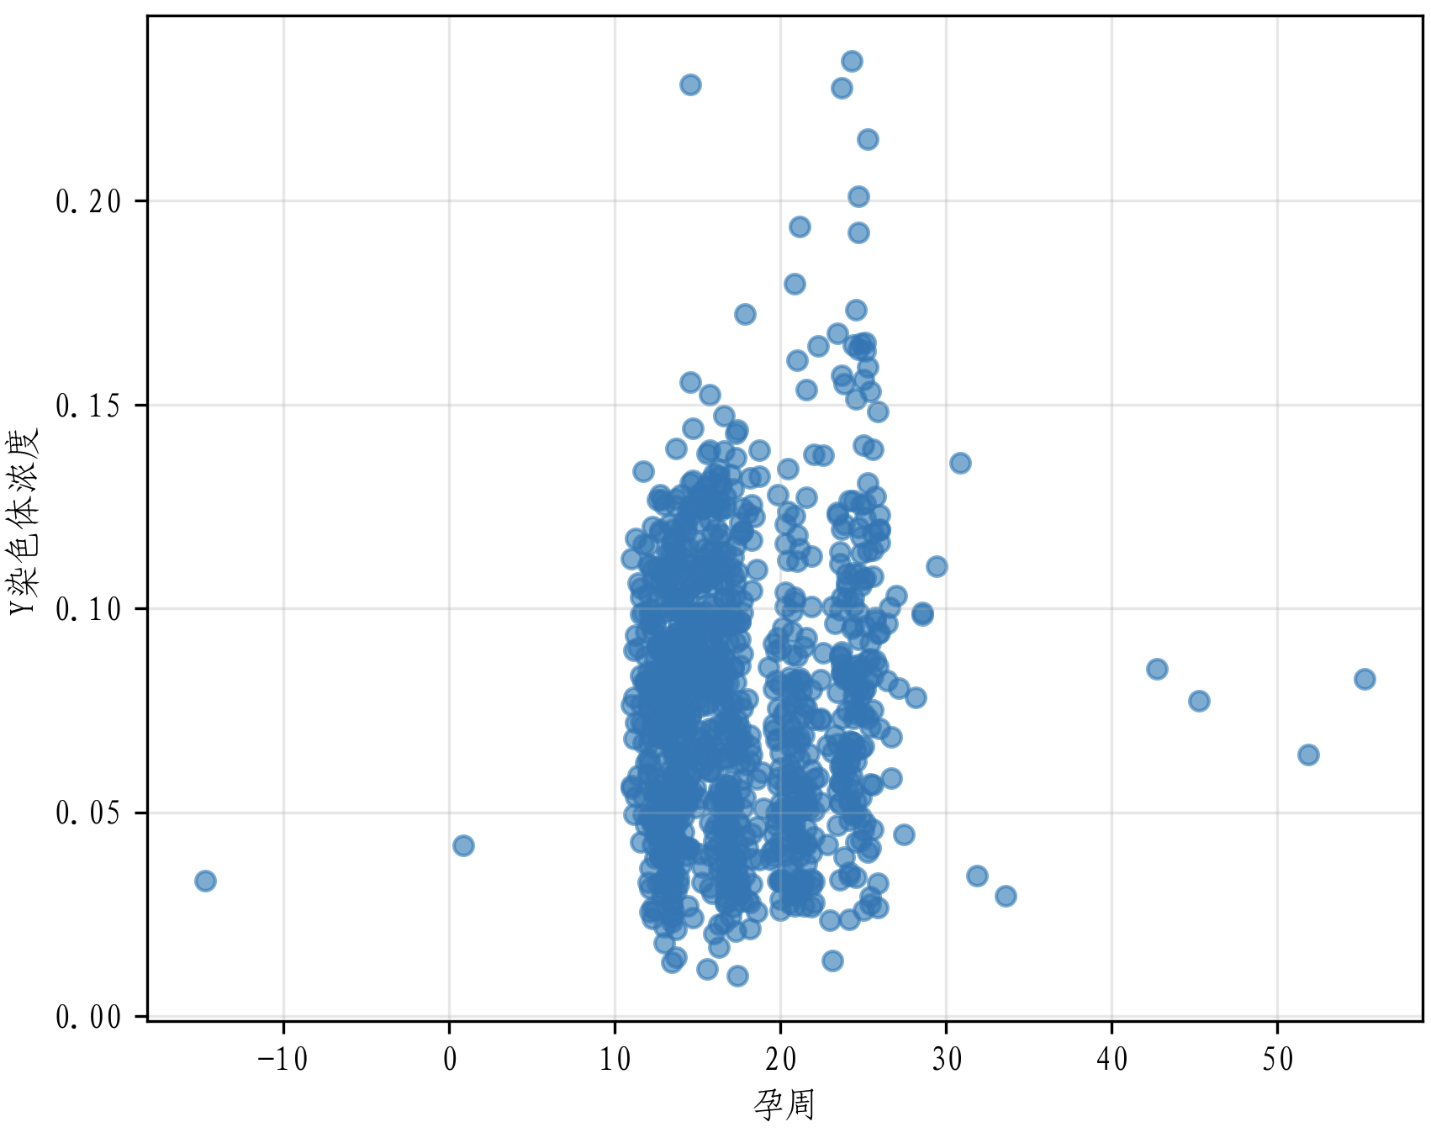
\includegraphics[width=0.8\textwidth]{../figure/q1_week_Yconc.png}
        \caption{孕周分布}
        \label{fig:孕周分布}
    \end{minipage}
    \begin{minipage}{0.49\textwidth}
        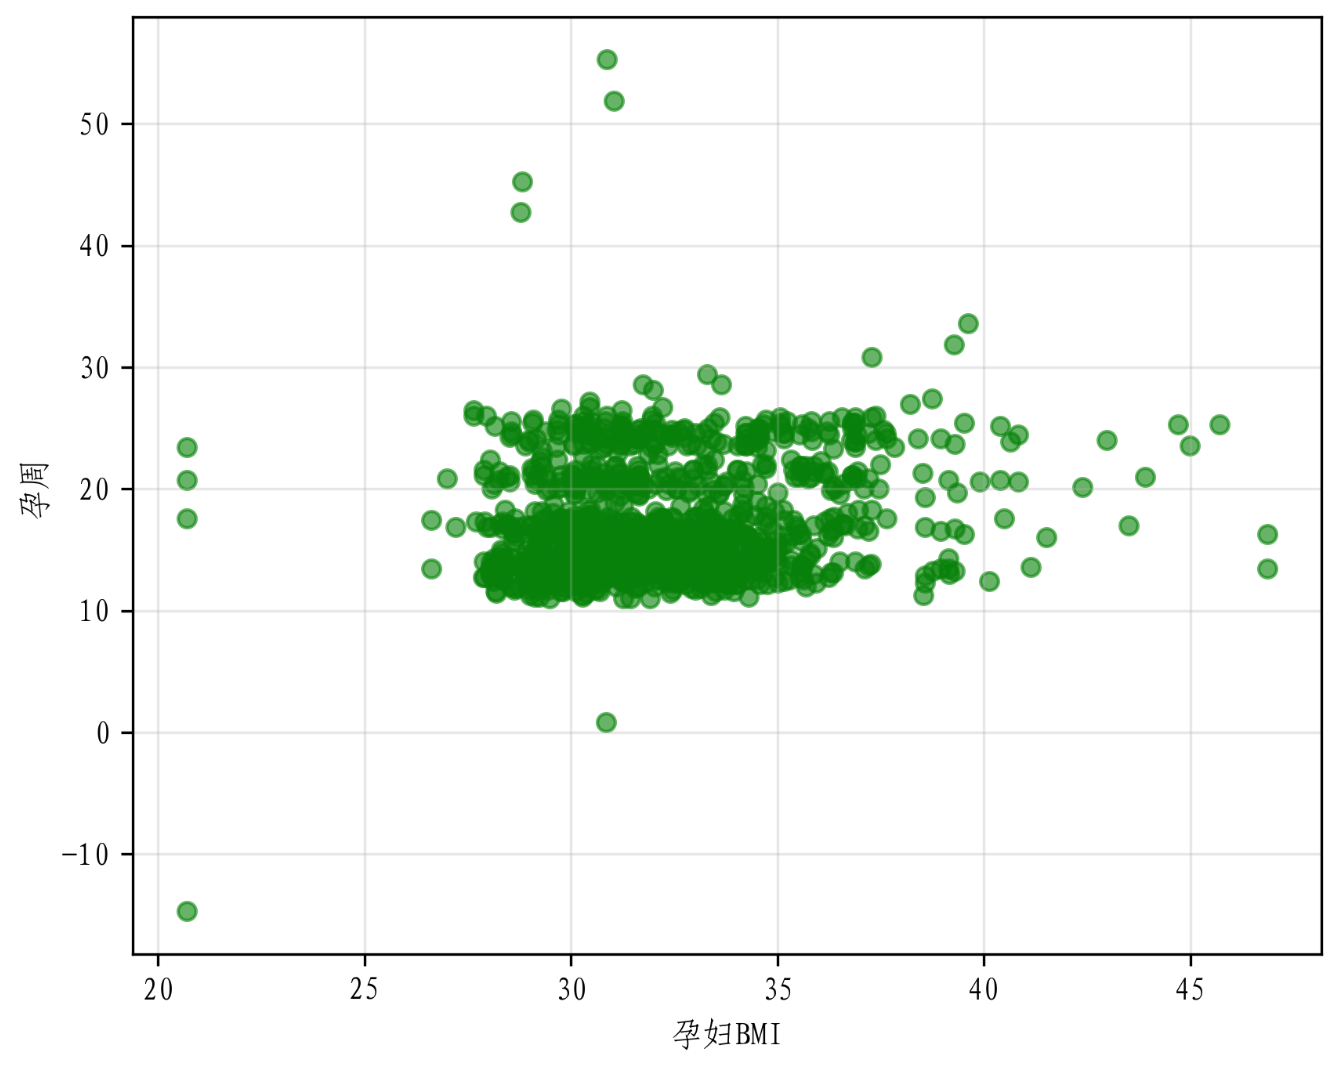
\includegraphics[width=0.8\textwidth]{../figure/q1_week_BMI.png}
        \caption{BMI分布}
        \label{fig:BMI分布}
    \end{minipage}
\end{figure}

由图\ref{fig:YandWbyBMI}分析可得Y 浓度总体呈现随孕周上升的趋势,但数据离散度较大,高 BMI 样本主要分布在低 Y 浓度区域;Y 浓度相对于 BMI 则表现出下降趋势,尤其在孕周较小时更为明显,且高 BMI 孕妇的 Y 浓度增长速度较慢。

\begin{figure}[H]
    \centering
    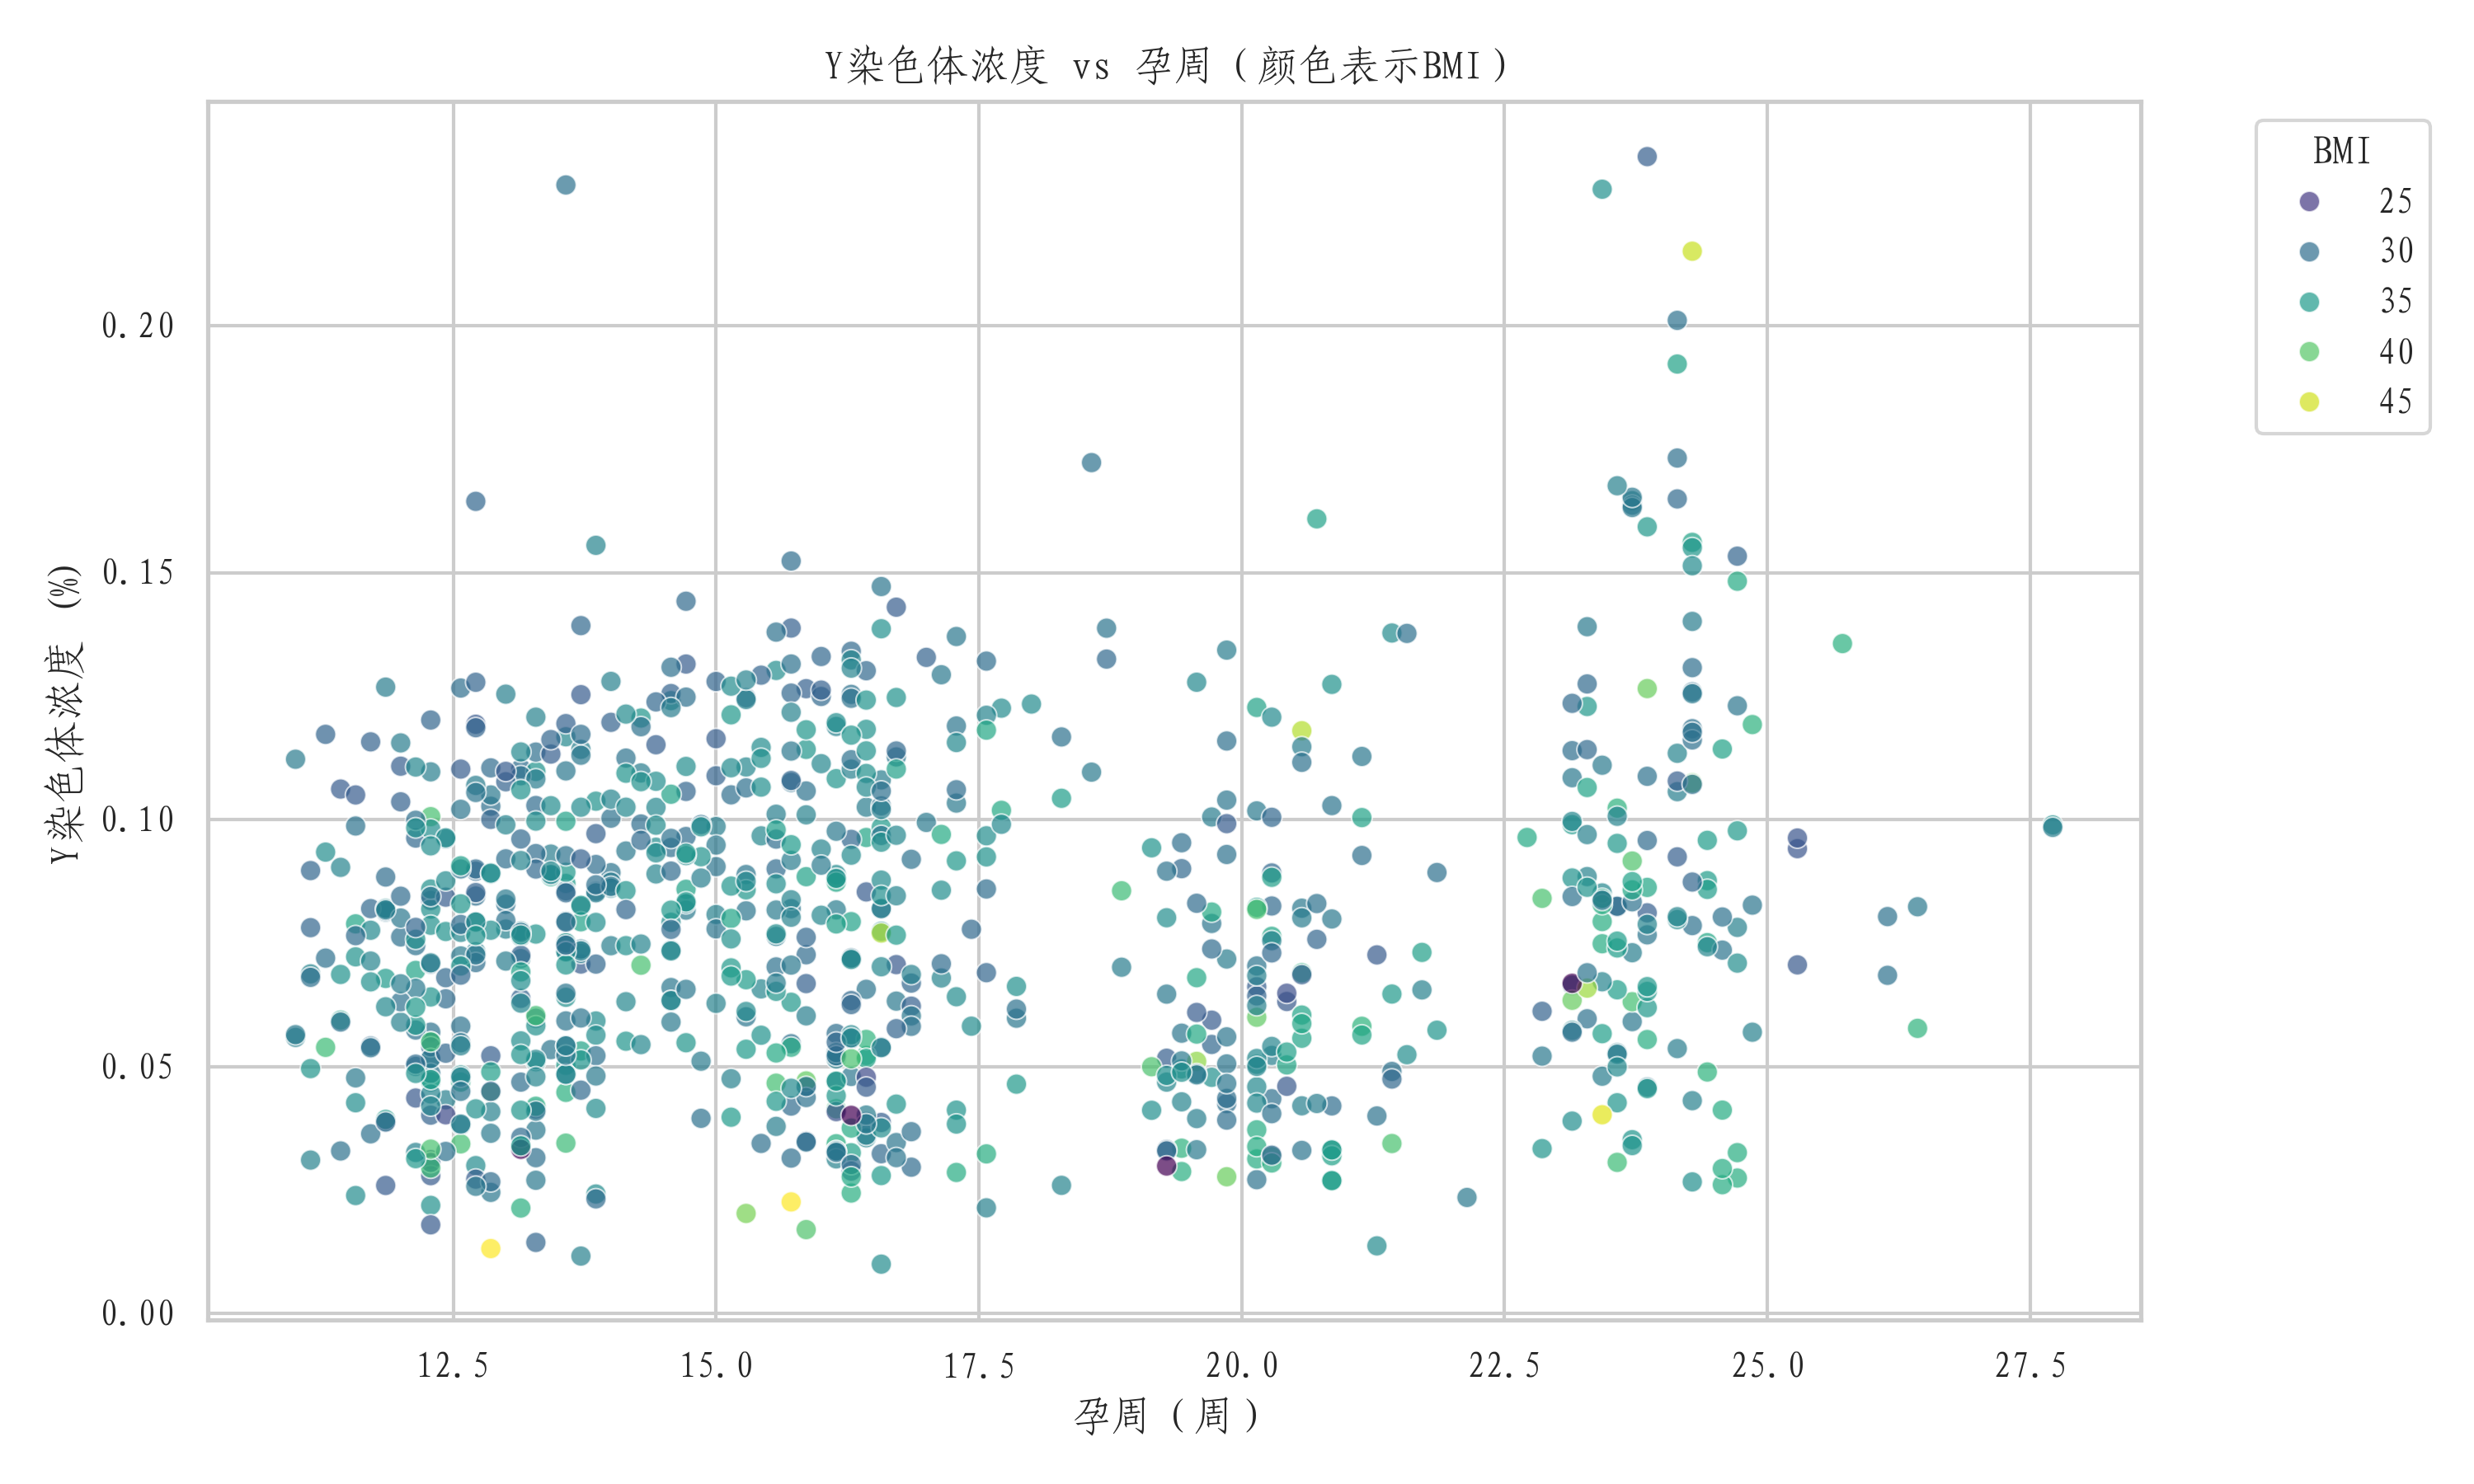
\includegraphics[width=0.8\textwidth]{../figure/q1_scatter_y_vs_gw_by_bmi.png}
    \caption{按 BMI 着色的 Y浓度 vs 孕周图}
    \label{fig:YandWbyBMI}
\end{figure}
计算包含 Y 染色体浓度、孕周、BMI、年龄关键变量的相关系数矩阵后,以热力图形式可视化其相关性,由图 \ref{fig:heatmap} 得出变量的相关性分析

\begin{enumerate}
    \item Y 染色体浓度与孕周相关系数为 +0.12,呈现弱正相关。这表明随着孕周的增加,Y 染色体浓度有一定程度的上升趋势,但这种关系并不十分强烈。
    \item Y 染色体浓度与BMI相关系数为 -0.13,呈现弱负相关。说明孕妇的 BMI 越高,Y 染色体浓度可能越低。
    \item Y 染色体浓度与孕妇年龄相关系数为 -0.12,可能反映了孕妇的年龄越大,Y染色体的浓度越低。
\end{enumerate}

\begin{figure}[H]
    \centering
    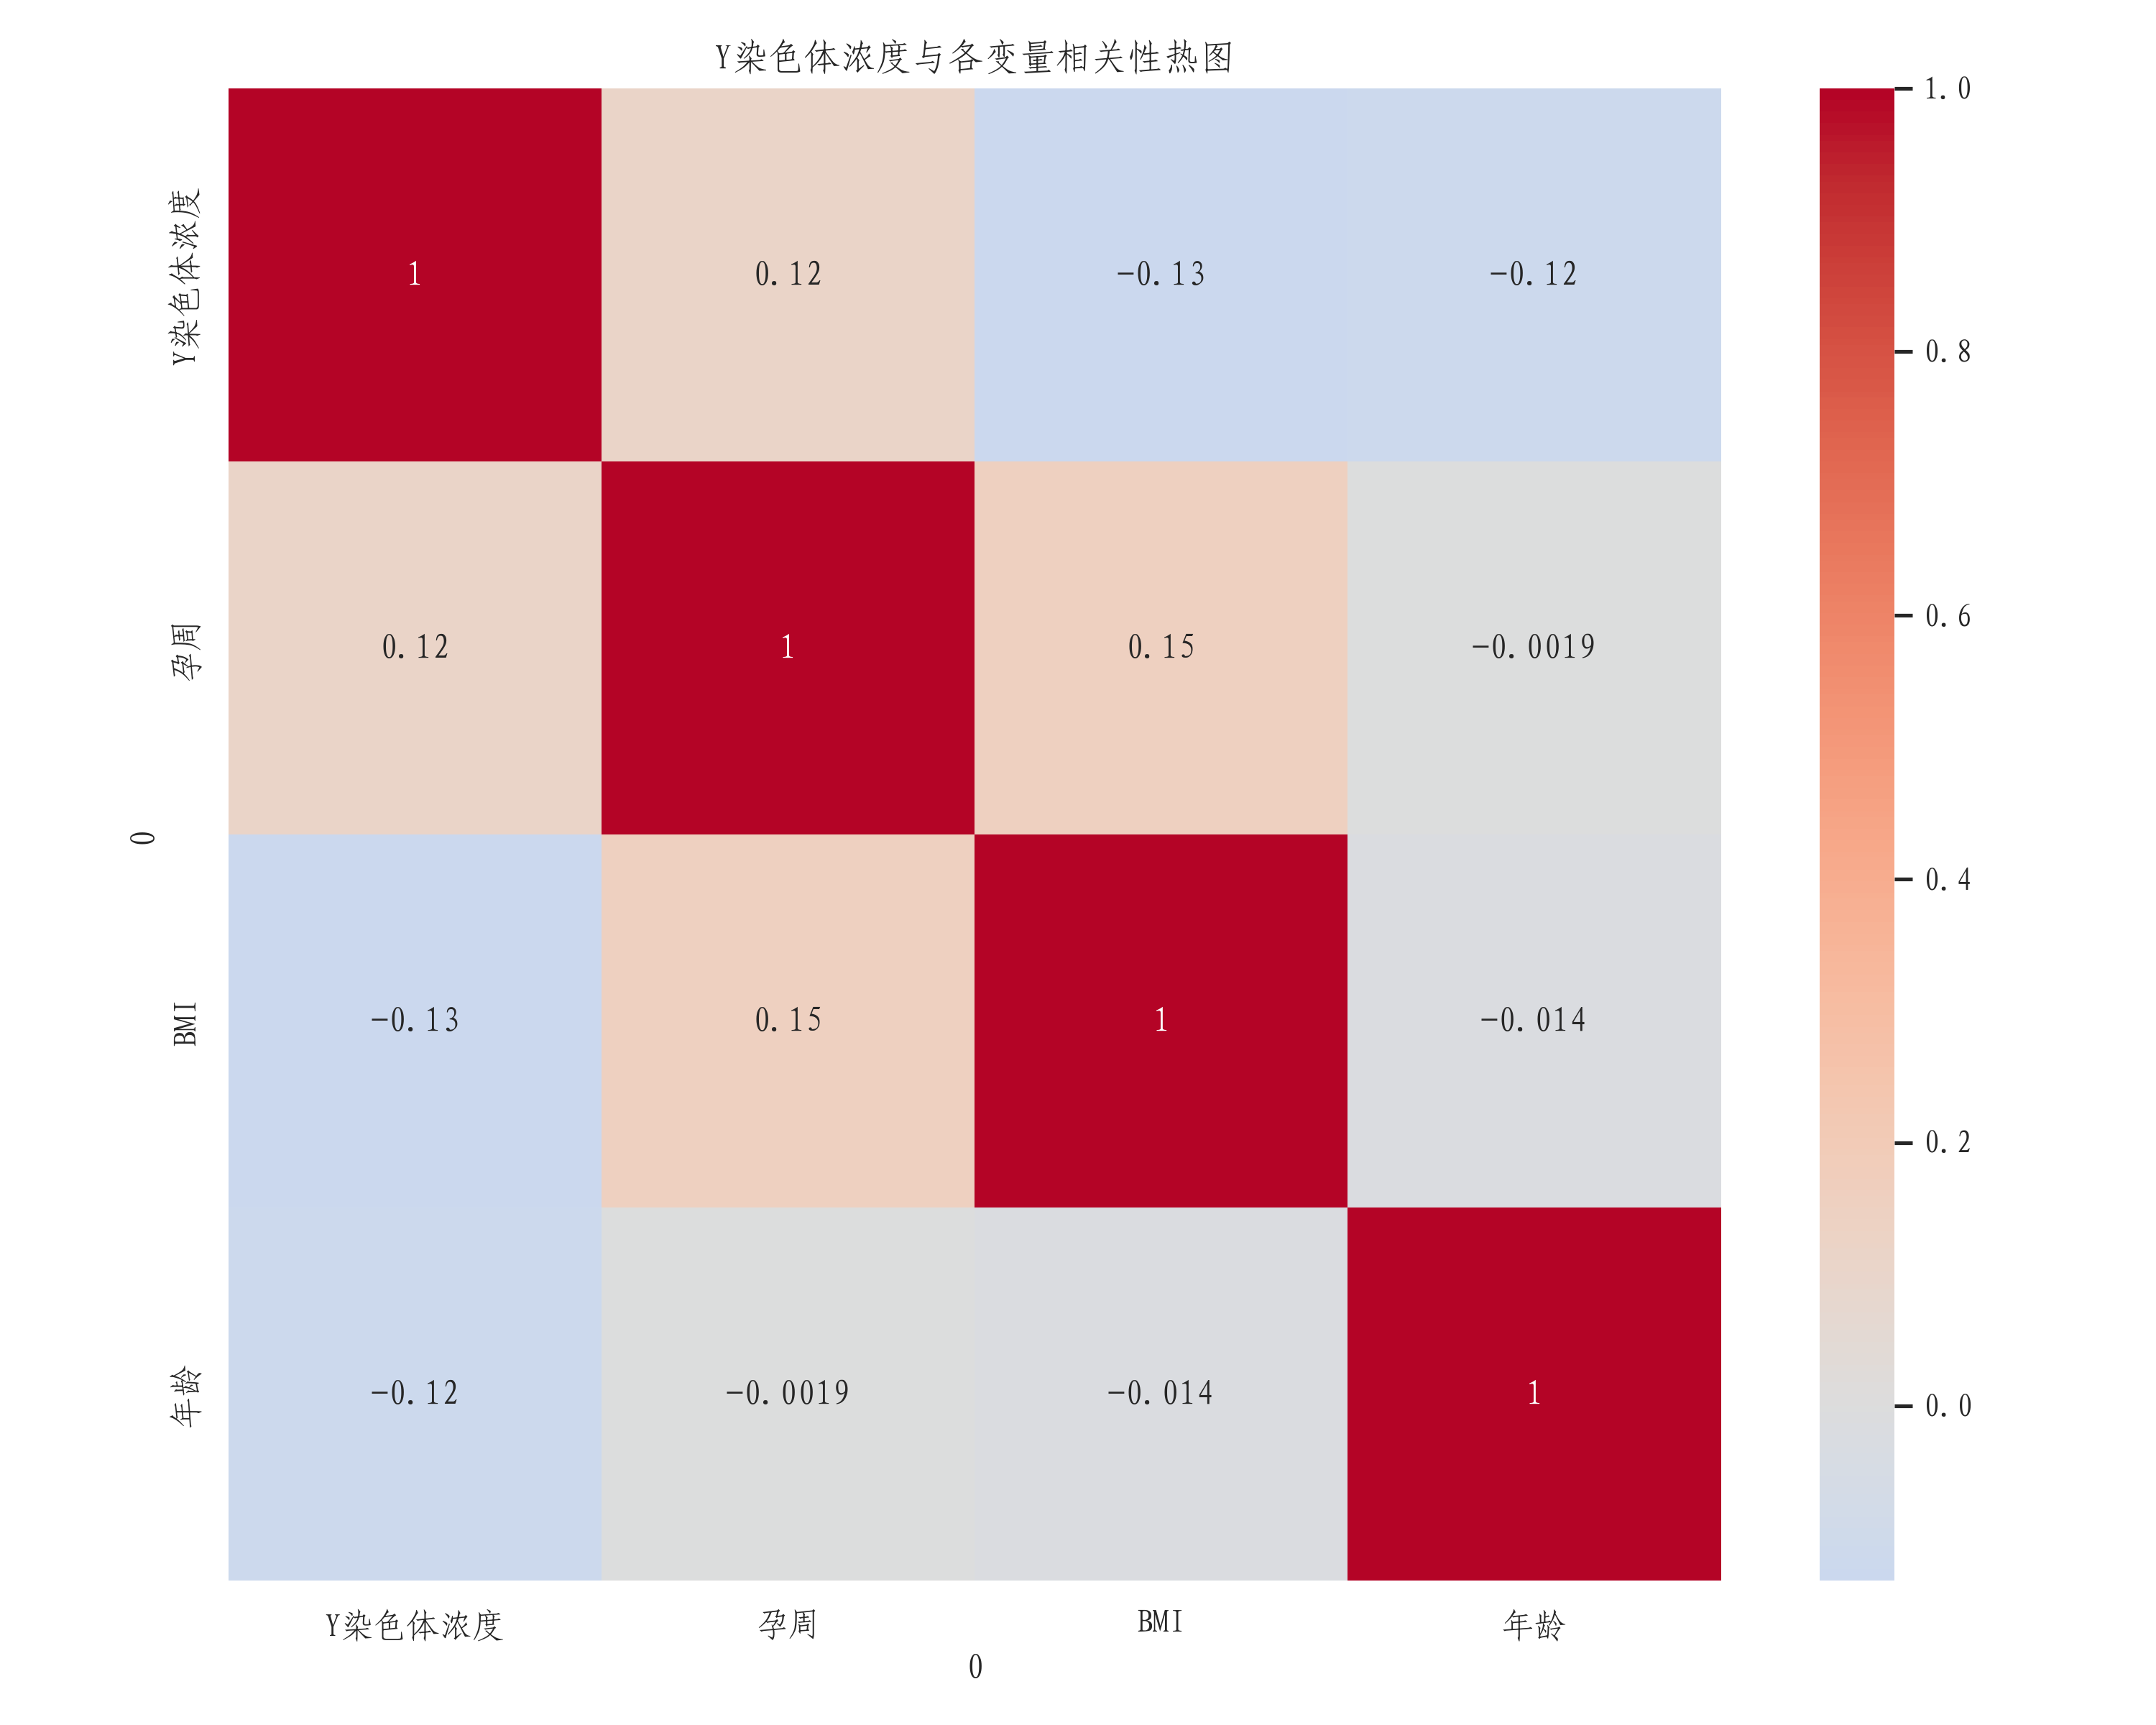
\includegraphics[width=0.6\textwidth]{../figure/q1_correlation_heatmap.png}
    \caption{相关性分析热力图}
    \label{fig:heatmap}
\end{figure}

\subsubsection{关系模型}
通过相关性分析,我们可以建立以下模型

\textbf{(一)多元线性回归模型}

通过分析相关性矩阵,我们发现 Y 染色体浓度和孕周之间有弱正相关($r=0.12$),而 Y 染色体浓度和 BMI 之间有弱负相关($r=-0.13$)。另外,两者之间没有严重的多重共线性问题(VIF<5),这表明可以用来构建多元线性回归模型。图 \ref{fig:YandWbyBMI} 也显示,Y 染色体浓度与孕周、Y 染色体浓度与 BMI 总体上呈现线性变化,没有明显的非线性波动。考虑到题目特别关注孕周和 BMI,我们先用这两个变量建立一个简单的线性模型,这样可以快速抓住基本的关联模式,也为后面更复杂的模型提供一个参考点,适合用来研究 Y 染色体浓度和这些核心指标的关系。该多元线性回归模型的公式为

\begin{equation}
    Y = \beta_0 + \beta_1 \cdot GW + \beta_2 \cdot BMI + \epsilon
\end{equation}
其中 $Y$ 为 Y 染色体浓度,$GW$ 为孕周,$BMI$ 为孕妇的身体质量指数,$\beta_0$ 为截距,$\beta_1$ 和 $\beta_2$ 为回归系数,$\epsilon$ 为误差项。对于这个模型,我们通过以下步骤来进行优化求解。

\textbf{Step 1}: 
基于相关性分析可知,$Y$与$GW$相关系数$r=0.12$,$Y$与$BMI$相关系数$r=-0.13$,先分别构建单变量模型。

当仅含GW时,模型表示为
\begin{equation}
    Y = \beta_{01} + \beta_{11} \cdot GW + \epsilon_1
\end{equation}

此时残差平方和为
\begin{equation}
    SSE_1 = \sum (Y_i \hat{Y}_{i1})^2
\end{equation}

当仅含BMI时,模型表示为
\begin{equation}
    Y = \beta_{02} + \beta_{12} \cdot BMI + \epsilon_2
\end{equation}

此时残差平方和为
\begin{equation}
    SSE_2 = \sum (Y_i \hat{Y}_{i2})^2
\end{equation}
    
\textbf{Step 2}:
因孕周与BMI无严重多重共线性(VIF<5),满足线性回归“无多重共线性假设”,将两个变量整合为多元线性模型,
模型表示为
\begin{equation}
    Y = \beta_0 + \beta_1 \cdot GW + \beta_2 \cdot BMI + \epsilon
\end{equation}

此时残差平方和为
\begin{equation}
    SSE = \sum (Y_i - (\beta_0 + \beta_1 \cdot GW_i + \beta_2 \cdot BMI_i))^2
\end{equation}

\textbf{Step 3}:
进行模型参数优化,通过最小化残差平方和来算参数,用最小二乘法得出

\begin{equation}
    \hat{\beta} = (X^TX)^{-1}X^TY
\end{equation}

其中$X = \begin{bmatrix} 1 & GW_1 & BMI_1 \\ 1 & GW_2 & BMI_2 \\ \vdots & \vdots & \vdots \\ 1 & GW_n & BMI_n \end{bmatrix}$为设计矩阵,$Y = [Y_1, Y_2, ..., Y_n]^T$为因变量向量。  

\textbf{Step 4}:
基于前一步优化的参数,验证残差正态性($\epsilon \sim N(0, \sigma^2)$)和方差齐性($Var(\epsilon_i) = \sigma^2$)均满足假设。F 检验显示模型整体显著($p=3.46 \times 10^{-8}$),表明该多元线性回归模型在统计上有效。最终确定的模型参数如表 \ref{tab:多元线性回归模型各项系数拟合结果} 所示。
从表中提取与 Y 染色体浓度关系的关键信息:
\begin{enumerate}
    \item 截距为 0.1150(p < 0.001),提供模型的基准值。
    \item 孕周的系数为 0.0012(p = $2.20 \times 10^{-5}$),显示正向影响显著,每单位孕周平均增加 Y 染色体浓度 0.0012%。
    \item BMI 的系数为 -0.0017(p = $2.90 \times 10^{-6}$),显示负向影响显著,每单位 BMI 平均减少 Y 染色体浓度 0.0017%。
\end{enumerate}

这些结果支持孕周和 BMI 分别对 Y 染色体浓度产生正向和负向显著影响。模型 $R^2 = 0.0367$(解释 3.67\% 数据变化),拟合效果有限,但 F 检验 p 值为 $3.17 \times 10^{-8}$
确认整体有效性。综上,该模型有效描述孕周和 BMI 的双重影响。


\begin{table}[H]
    \centering
    \caption{多元线性回归模型各项系数拟合结果}
    \label{tab:多元线性回归模型各项系数拟合结果}
    \begin{threeparttable}
        \begin{tabularx}{0.55\textwidth}{l c c c c c}
            \toprule[1.5pt]
            \textbf{变量} & \textbf{系数} & \textbf{标准差} & \textbf{t值} & \textbf{p值}\\
            \midrule[1pt]
            截距 & 0.1150 & 0.012 & 9.505 & 0.000  \\
            孕周 & 0.0012 & 0.0003 & 4.266 & $2.20 \times 10^{-5}$  \\
            BMI  & -0.0017 & 0.0004  & -4.707 & $2.90 \times 10^{-6}$  \\
            \bottomrule[1.5pt]
        \end{tabularx}
    \end{threeparttable}
\end{table}


\textbf{(二)多项式 + 交互项模型}

因为线性模型有局限性,而且变量之间有特殊关联,我们发现一方面,线性模型的贴合度不高($R^2=0.0367$),散点图还显示 Y 染色体浓度和孕周的关系后期增长变慢,需引入 $GW^2$项来捕捉这个曲线趋势;另一方面,按 BMI 着色的散点图表明,不同 BMI 组里孕周对 Y 浓度的影响斜率不一样,如低 BMI 组斜率陡一些,说明 BMI 可能在调节孕周的影响,需引入“孕周×BMI”交互项来反映这个关系。加了这些项后,模型能更好地解释数据里的复杂联系,弥补线性模型的拟合不足。具体公式是为
\begin{equation}
    \label{eq:多项式 + 交互项模型}
    Y = \beta_0 + \beta_1 \cdot GW + \beta_2 \cdot GW^2 + \beta_3 \cdot BMI + \beta_4 \cdot (GW \times BMI) + \epsilon
\end{equation}

该模型的 $R^2 = 0.0410$,相比线性回归模型有一定提升,说明增加多项式和交互项后,模型对数据的拟合能力有所增强。F 检验 p 值为 $8.46 \times 10^{-8}$,表明模型整体显著。然而,仅 BMI 变量在 $\alpha = 0.05$ 水平下显著,孕周主效应和交互项不太明显,于是我们按如下步骤对这个模型进行优化求解。

\textbf{Step 1}:散点图显示 Y 浓度和孕周有“先缓后稳”的非线性趋势,因此基于线性模型引入非线性项$GW^2$来反映二次效应,构建多项式模型式

\begin{equation}
    Y = \beta_0 + \beta_1 \cdot GW + \beta_2 \cdot GW^2 + \beta_3 \cdot BMI + \epsilon_3
\end{equation}

此时,残差平方和
\begin{equation}
    SSE_3 = \sum (Y_i - (\beta_0 + \beta_1 \cdot GW_i + \beta_2 \cdot GW_i^2 + \beta_3 \cdot BMI_i))^2
\end{equation}

\textbf{Step 2}:按 BMI 分组的散点图显示 BMI 可能在调节孕周对 Y 浓度的影响,因此引入交互项$GW \times BMI$刻画调节效应,模型扩展为:
  \begin{equation}
    Y = \beta_0 + \beta_1 \cdot GW + \beta_2 \cdot GW^2 + \beta_3 \cdot BMI + \beta_4 \cdot (GW \times BMI) + \epsilon
  \end{equation} 
  
  此时残差平方和
  \begin{equation}
    SSE_4 = \sum (Y_i - (\beta_0 + \beta_1 \cdot GW_i + \beta_2 \cdot GW_i^2 + \beta_3 \cdot BMI_i + \beta_4 \cdot GW_i \cdot BMI_i))^2
  \end{equation}

\textbf{Step 3}:采用最小二乘法求解参数,同时计算变量方差膨胀因子(VIF)来进行参数优化与多重共线性处理,发现因$GW$与$GW^2$、$GW \times BMI$存在一定相关性,条件数达$3.23 \times 10^4$,但核心变量(BMI)仍显著($p=0.017$),因此暂时不用剔除变量。

\textbf{Step 4}:F检验显示模型整体显著($p=8.46 \times 10^{-8}$),$R^2$提升至0.041,最终确定多项式+交互项模型各项参数如表\ref{tab:多项式 + 交互项模型各项系数拟合结果}所示。

\textbf{Step 4}:模型显著性验证与最终确定
F 检验显示模型整体显著($p=8.46 \times 10^{-8}$),表明该多项式 + 交互项模型在统计上有效。$R^2$ 提升至 0.041,说明模型解释了约 4.1\% 的数据变化,拟合效果略有改善。最终确定的模型参数如表 \ref{tab:多项式 + 交互项模型各项系数拟合结果} 所示。
从表中提取与 Y 染色体浓度关系的关键信息:
\begin{enumerate}
    \item 截距为 0.2114(p = 0.000),提供模型的基准值。
    \item 孕周的系数为 -0.0061(p = 0.093),直接影响不显著。
    \item 孕周² 的系数为 $9.77 \times 10^{-5}$(p = 0.186),二次效应不显著。
    \item BMI 的系数为 -0.0038(p = 0.017),显示负向影响显著,每单位 BMI 平均减少 Y 染色体浓度 0.0038\%。
    \item 孕周×BMI 交互项的系数为 $1.0 \times 10^{-4}$(p = 0.183),交互效应不显著。
\end{enumerate}
这些结果表明 BMI 是唯一显著影响 Y 染色体浓度的变量,添加的二次项和交互项未能显著提升模型表现。模型 $R^2 = 0.041$ 比线性模型略高,但整体拟合提升有限。综上,该模型在 BMI 效应上优于线性模型,但非线性改进不明显。




\begin{table}[H]
    \centering  % 表居中
    \caption{多项式 + 交互项模型各项系数拟合结果}  % 表标题
    \label{tab:多项式 + 交互项模型各项系数拟合结果}  % 表标签
    \begin{threeparttable}
        % 表内容
        \begin{tabularx}{0.4\textwidth}{l c c }
            \toprule[1.5pt]
            \textbf{变量} & \textbf{系数} & \textbf{p值}\\ 
            \midrule[1pt]
            截距 & 0.2114 & 0.000  \\
            孕周 & -0.0061 & 0.093  \\
            孕周² & $9.77 \times 10^{-5}$ & 0.186  \\
            BMI & -0.0038 & 0.017  \\
            孕周×BMI & $1.0 \times 10^{-4}$ & 0.183  \\        \bottomrule[1.5pt]
    \end{tabularx}
\end{threeparttable}
\end{table} 




\subsubsection{显著性检验}




\subsection{问题二模型的建立与求解}


\subsubsection{模型构建} 
参考临床BMI分类(正常<28,超重28-32,肥胖>32),结合数据中高BMI样本占比高的特点,兼顾医学合理性与数据分布特征,将孕妇BMI值细化至5个区间,每组样本量需满足统计有效性(最小组样本数$\ge$3,本模型中各组样本数为3-143,均符合要求),函数表示如下
\begin{equation}
    g = \begin{cases} 
1, & 20 \leq BMI_i < 28 \\
2, & 28 \leq BMI_i < 32 \\
3, & 32 \leq BMI_i < 36 \\
4, & 36 \leq BMI_i < 40 \\
5, & BMI_i \geq 40 
\end{cases}
\end{equation}

定义首次达标孕周为对孕妇$i$,$T_i = \min\{t \mid Y_{i,t}≥\theta\}$(即首次满足浓度达标的最小孕周)。对每组$g$,计算$T_i$的关键分位值(80分位、90分位),其中80分位值$t_{g,0.8}$表示“该组内80\%孕妇已达标的最晚孕周”,公式为
\begin{equation}
    t_{g,0.8} = \inf\left\{ t \mid P(T_i \leq t \mid g) \geq 0.8 \right\}
\end{equation}

所以可得目标函数为在保证达标比例≥80\%(准确性)的前提下,最小化检测孕周(降低风险),即  
\begin{align}
\min_{t_g} \quad t_g \\
\text{s.t.} \quad P(T_i \leq t_g \mid g) \geq 0.8 \\
8 \leq t_g \leq 28
\end{align}


约束条件要求$t_g$需覆盖组内80\%孕妇的达标时间,因此最优解为该组$T_i$的80分位值$t_{g,0.8}$,即$t_g^* = t_{g,0.8}$,若80分位值超出“中期早期”(13-16周),需验证90分位值是否进入高风险区间,确保时点选择在“风险-准确性”平衡点。为量化误差对最佳时点的影响,构建误差修正模型。考虑±0.5周的时间记录偏差,最佳时点的置信区间为:  
\begin{equation}
[t_g^* - \Delta t, t_g^* + \Delta t]
\end{equation}
另外,模拟±5\%的浓度相对误差($\hat{Y}_{i,t} = Y_{i,t} \times (1+\Delta Y)$),重新计算达标时间$T_i'$,验证80分位值$t_{g,0.8}'$与原时点$t_{g,0.8}$的差异。  


\subsubsection{模型求解} 
读取问题一清洗后的男胎数据表,初始样本926例,  首次达标时间的计算按孕妇编号分组,取“达标”状态下的最小孕周作为$T_i$。通过分组函数对260名孕妇进行分组,各组样本分布如表\ref{tab:按BMI分组后各组情况表}所示。

\begin{table}[H]
    \centering  % 表居中
    \caption{按BMI分组后各组情况表}  % 表标题
    \label{tab:按BMI分组后各组情况表}  % 表标签
    \begin{threeparttable}
        % 表内容
        \begin{tabularx}{0.62\textwidth}{c c l c c }
            \toprule[1.5pt]
            \textbf{分组$g$} & \textbf{BMI区间} & \textbf{临床分类} & \textbf{孕妇数量} & \textbf{占比}\\ 
            \midrule[1pt]
            1       & [20,28)    & 正常       & 5        & 1.9\%   \\
            2       & [28,32)    & 超重       & 143      & 55.0\%  \\
            3       & [32,36)    & 肥胖       & 92       & 35.4\%  \\
            4       & [36,40)    & 重度肥胖   & 17       & 6.5\%   \\
            5       & ≥40        & 极重度肥胖 & 3        & 1.2\%   \\

            \bottomrule[1.5pt]
        \end{tabularx}
    \end{threeparttable}
\end{table}

对每组数据计算$T_i$统计指标(均值、中位、80分位、90分位),计算结果如表\ref{tab:各BMI组统计指标计算结果}所示。
\begin{table}[H]
    \centering  % 表居中
    \caption{各BMI组统计指标计算结果}  % 表标题
    \label{tab:各BMI组统计指标计算结果}  % 表标签
    \begin{threeparttable}
        % 表内容
        \begin{tabularx}{0.9\textwidth}{c c c c }
            \toprule[1.5pt]
            \textbf{分组$g$} & \textbf{BMI区间} & \textbf{平均达标孕周(周)} & \textbf{中位达标孕周(周)} \\ 
            \midrule[1pt]
            1 & [20,28) & 13.94 & 12.71  \\  
            2 & [28,32) & 14.07 & 12.86  \\  
            3 & [32,36) & 32-36 & 13.14  \\  
            4 & [36,40) & 36-40 & 15.57  \\  
            5 & ≥40     & ≥40   & 17.71  \\  
            \bottomrule[1.5pt]
        \end{tabularx}
        \begin{tabularx}{0.9\textwidth}{c c c c }
            \textbf{分组$g$} & \textbf{BMI区间} & \textbf{80分位达标孕周$t_{g,0.8}$(周)} & \textbf{90分位达标孕周(周)}\\ 
            \midrule[1pt]
            1 & [20,28)  & 16.17 & 16.23 \\  
            2 & [28,32)  & 16.14 & 18.96 \\  
            3 & [32,36)  & 13.83 & 16.40 \\  
            4 & [36,40)  & 17.06 & 20.17 \\  
            5 & ≥40      & 18.83 & 19.20 \\  
            \bottomrule[1.5pt]
        \end{tabularx}
    \end{threeparttable}
\end{table}



根据优化模型,每组最佳时点为80分位达标孕周$t_{g,0.8}$,转换为“周+天”格式便于临床应用,转换结果如表\ref{tab:建议检测时间表}。

\begin{table}[H]
    \centering  % 表居中
    \caption{建议检测时间表}  % 表标题
    \label{tab:建议检测时间表}  % 表标签
    \begin{threeparttable}
        % 表内容
        \begin{tabularx}{0.94\textwidth}{c c l c c }
            \toprule[1.5pt]
            \textbf{分组$g$} & \textbf{BMI区间} & \textbf{最佳NIPT时点$t_g^*$(周)} & \textbf{建议检测时间} & \textbf{对应风险等级}\\ 
            \midrule[1pt]
            1 & [20,28)  & 16.17 & 16周1天  & 中期早期    \\
            2 & [28,32)  & 16.14 & 16周0天  & 中期早期    \\
            3 & [32,36)  & 13.83 & 13周5天  & 中期早期\\
            4 & [36,40)  & 17.06 & 17周0天  & 中期        \\
            5 & ≥40      & 18.83 & 18周5天  & 中期        \\
            \bottomrule[1.5pt]
        \end{tabularx}
    \end{threeparttable}
\end{table}


关于检测误差稳健性验证,在时间误差方面,最佳时点的置信区间均在安全范围内,未进入晚期(≥28周),如表\ref{tab:误差检验}所示,在浓度误差影响:添加±5\%浓度噪声后,各组80分位达标时间与原时点完全一致(如分组3仍为13.83周),说明模型对浓度测量误差的抗干扰能力强。

\begin{table}[H]
    \centering  % 表居中
    \caption{建议检测时间表}  % 表标题
    \label{tab:误差检验}  % 表标签
    \begin{threeparttable}
        % 表内容
        \begin{tabularx}{0.8\textwidth}{c c c c c }
            \toprule[1.5pt]
            \textbf{分组$g$} & \textbf{最佳时点(周)} & \textbf{置信区间(周)} & \textbf{置信区间(周+天)}\\ 
            \midrule[1pt]
            1 & 16.17 & [15.67,16.67] & [15周4天,16周4天] \\ 
            2 & 16.14 & [15.64,16.64] & [15周4天,16周4天] \\ 
            3 & 13.83 & [13.33,14.33] & [13周2天,14周2天] \\ 
            4 & 17.06 & [16.56,17.56] & [16周4天,17周4天] \\ 
            5 & 18.83 & [18.33,19.33] & [18周2天,19周2天] \\ 
            \bottomrule[1.5pt]
        \end{tabularx}
    \end{threeparttable}
\end{table}




通过以上对男胎孕妇按BMI分组的合理性、最佳NIPT检测时点的医学价值及检测误差影响的分析结论如下:
在分组合理性方面,所划分的[20,28)(正常)、[28,32)(超重)、[32,36)(肥胖)、[36,40)(重度肥胖)、≥40(极重度肥胖)五组,既与临床BMI分类标准高度契合,细化的重度肥胖、极重度肥胖组别又符合高BMI地区孕妇的实际分布特征,且各组样本量均满足统计分析要求(最小3例),通过80分位值刻画群体达标规律还能有效避免极端值干扰,确保了分组的科学性与数据有效性;

在最佳时点的医学意义上,呈现出“BMI越高,最佳检测时点越晚”的清晰趋势,这与“BMI与Y染色体浓度负相关”的生理机制一致——高BMI孕妇胎盘屏障功能可能较弱,胎儿游离DNA进入母体血液的速度较慢,同时所有组的最佳时点均控制在“中期早期(13-18周)”,未进入风险更高的“中期晚期(19-27周)”及“晚期(≥28周)”,实现了风险的最大限度降低,其中[32,36)组(肥胖)最佳时点为13周5天,接近“早期(≤12周)”窗口,推测与该组孕妇特定代谢特征导致Y浓度增长速度最快有关;

在检测误差影响方面,±0.5周的时间误差和±5\%的浓度误差均未改变最佳时点所属的风险等级,证明模型具有良好的稳健性,仅针对极重度肥胖组(≥40),建议实际检测时可适当提前0.5周(从18周5天调整为18周2天),以进一步降低其进入中期晚期的潜在风险 。




\subsection{问题三模型的建立与求解}
\subsubsection{模型构建}
经过分析知,因变量“Y达标”为二分类变量(0/1),且核心目标是预测“达标概率”随各因素的变化规律,而逻辑回归能直接输出概率值,便于与“90\%达标概率”的目标结合,且通过logit变换将非线性的概率关系转化为线性模型,便于解释各因素的影响方向与强度,此外还有模型参数少,计算简便且易于验证稳健性的特点,因此逻辑回归是最优选择。

基于变量选择结果(孕周、BMI、年龄、身高、体重、GC含量),构建多元逻辑回归模型:  
\begin{equation}
    \text{logit}(P) = \beta_0 + \beta_1X_1 + \beta_2X_2 + \beta_3X_3 + \beta_4X_4 + \beta_5X_5 + \beta_6X_6
\end{equation}
其中:$\beta_0$为截距项,反映所有自变量为0时的logit(P)基准值,$\beta_i$($i=1,...,6$)为回归系数,正系数表示该变量增大时,达标概率上升($\text{logit}(P)$增大),负系数则相反。  
在变量选择依据上,核心变量有孕周($X_1$)、BMI($X_2$),题目明确要求分析的关键因素,问题2已验证二者对达标时间的显著影响;协变量有年龄($X_3$)、身高($X_4$)、体重($X_5$)以及GC含量($X_6$)。  

为评估模型的性能,选取以下指标作为评价标准:
\begin{enumerate}
    \item AUC(Area Under ROC Curve):衡量模型分类性能,AUC=0.5为随机水平,AUC≥0.7为良好;
    \item Pseudo $R^2$:类比线性回归的$R^2$,反映模型对因变量变异的解释能力;
    \item LLR p-value(似然比检验p值):检验模型整体显著性,p<0.05表示模型优于空模型(无自变量);
    \item 分组AUC:按BMI分组计算AUC,评估模型在不同群体中的预测效果差异。
\end{enumerate}
  

\subsubsection{模型求解}  
读取问题1清洗后的数据表,包含926例样本,对每条数据达标状态标记:$Y=1$(Y染色体浓度≥0.04),$Y=0$(否则)BMI分组:按[20,28),[28,32),[32,36),[36,40),≥40划分为5组,标签为$g=1$到$g=5$。采用statsmodels库拟合逻辑回归模型,输出核心结果如表\ref{tab:模型拟合输出核心结果}所示。

\begin{table}[H]
    \centering  % 表居中
    \caption{逻辑回归模型输出核心结果}  % 表标题
    \label{tab:模型拟合输出核心结果}  % 表标签
    \begin{threeparttable}
        % 表内容
        \begin{tabularx}{0.9\textwidth}{c c c c c c c}
            \toprule[1.5pt]
            \textbf{变量} & \textbf{系数$\beta_i$} & \textbf{标准误} & \textbf{z值}& \textbf{p值}& \textbf{影响方向}& \textbf{显著性}\\ 
            \midrule[1pt]
            截距($\beta_0$)&  -57.8469& 34.069  & -1.698 & 0.090  & -     & 边缘显著\\  
            孕周($X_1$)    & 0.0344  & 0.026   & 1.314  & 0.189  & 正向    & 不显著   \\ 
            孕妇BMI($X_2$) &  0.9542  & 0.490   & 1.948  & 0.051  & 正向    & 显著    \\  
            年龄($X_3$)    & -0.0280 & 0.027   & -1.040 & 0.298  & 负向    & 不显著   \\ 
            身高($X_4$)    & 0.3813  & 0.196   & 1.946  & 0.052  & 正向    & 边缘显著 \\ 
            体重($X_5$)    & -0.4013 & 0.186   & -2.161 & 0.031  & 负向    & 显著     \\ 
            GC含量($X_6$)  & 3.8399  & 30.545  & 0.126  & 0.900  & 正向    & 无影响   \\ 
            \bottomrule[1.5pt]
        \end{tabularx}
    \end{threeparttable}
\end{table}
关于选定的模型性能指标,AUC结果为0.618,说明模型分类性能中等,优于随机猜测(0.5),但仍有提升空间;Pseudo $R^2=0.03392$,指出模型解释力较弱,说明Y染色体达标概率还受未纳入变量(如胎盘功能、代谢水平)影响;LLR p-value=0.0006294:模型整体显著(p<0.01),表明纳入的多因素联合对达标概率有显著预测作用;分组AUC:高BMI组预测效果更好([36,40)组AUC=0.703,≥40组AUC=0.705),低BMI组较差([20,28)组AUC=0.422),原因是低BMI组样本量少(仅5例),模型拟合不足。  

对每个BMI组,固定该组的BMI、年龄、身高、体重、GC含量(取组内均值),通过模型预测不同孕周(10-25周,间隔0.5周)的达标概率$P$,找到首次满足$P≥0.9$的最小孕周,即为该组的最佳时点$t_g^*$。求解结果如表\ref{tab:模型预测最佳检查时点}所示。

\begin{table}[H]
    \centering  % 表居中
    \caption{模型预测最佳检查时点}  % 表标题
    \label{tab:模型预测最佳检查时点}  % 表标签
    \begin{threeparttable}
        % 表内容
        \begin{tabularx}{\textwidth}{c c c c c c}
            \toprule[1.5pt]
            \textbf{BMI分组} & \textbf{最佳时点$t_g^*$(周)} & \textbf{建议检测时间} & \textbf{预测依据}& \textbf{风险等级}\\ 
            \midrule[1pt]
            $[20,28)$ & 21.5 & 21周3天 & 21.5周时$P=0.902$ & 中期     \\  
            $[28,32)$ & 13.0 & 13周0天 & 13.0周时$P=0.905$ & 中期早期   \\
            $[32,36)$ & 14.0 & 14周0天 & 14.0周时$P=0.901$ & 中期早期   \\
            $[36,40)$ & 15.0 & 15周0天 & 15.0周时$P=0.903$ & 中期早期   \\
            $≥40    $ & 10.0 & 10周0天 & 10.0周时$P=0.900$ & 异常(需验证)\\ 
            \bottomrule[1.5pt]
        \end{tabularx}
    \end{threeparttable}
\end{table}

对于≥40的异常结果组建议10周检测(早期窗口),与“高BMI孕妇达标时间晚”的常识矛盾,原因:  
样本量极少(仅3例),组内均值代表性不足;模型对极端BMI组的拟合偏差,需结合临床经验调整为16-18周(参考[36,40)组时点趋势)。  


模拟±5\%的浓度测量误差($\hat{Y}_{\text{浓度}}=Y_{\text{浓度}} \times \text{uniform}(0.95,1.05)$),重新拟合模型并评估性能后有以下结论:
\begin{enumerate}
    \item 误差后模型AUC=0.623(原AUC=0.618),变化极小;  
    \item 各变量回归系数显著性无变化(BMI、体重仍显著,孕周、年龄仍不显著);  
    \item 最佳时点仅[20,28)组从21.5周变为22.0周,其他组无变化。 
    \item 模型对±5\%的浓度误差具有较强稳健性,推荐时点可靠。
\end{enumerate} 


在模型结果分析中,各因素对Y染色体浓度达标概率的影响机制呈现出鲜明特征与内在关联,BMI虽呈正向显著影响($\beta_2=0.9542$),即BMI越高$\text{logit}(P)$越大,看似与“高BMI孕妇Y浓度更低、达标更难”的临床常识矛盾,但实则因模型中BMI与体重存在负向交互作用(体重$\beta_5=-0.4013$),高BMI若由“身高矮”而非“体重大”导致,反而可能间接提升达标概率,需结合BMI构成综合解读;体重呈负向显著影响($\beta_5=-0.4013$),体重越高$\text{logit}(P)$越小、达标概率越低,这与“体重越大,胎儿游离DNA在母体血液中稀释越严重、浓度越低”的生理机制完全契合;身高呈边缘显著正向影响($\beta_4=0.3813$),身高越高达标概率越高,推测因身高高的孕妇体脂分布更均匀,胎盘功能更稳定,更利于胎儿DNA释放;孕周虽呈正向趋势(孕周越大达标概率越高),但未达显著水平($\beta_1=0.0344$),核心原因是模型纳入的BMI、体重等因素对达标概率的影响更强,掩盖了孕周的独立作用。从最佳时点合理性来看,与问题2基于80\%分位值的结果相比,问题3基于90\%达标概率的时点整体略有推迟,如[28,32)组因多因素模型捕捉到该组体重较低的优势,时点从16周提前至13周,高BMI组[36,40)则因模型纳入体重后发现该组体重均值较低、达标速度快于单纯BMI分组预期,时点从17周提前至15周;从临床适配性而言,[28,32)、[32,36)、[36,40)组时点均处于13-15周的“中期早期”,完美契合“尽早检测且保证准确性”的核心目标,而[20,28)组21.5周的时点虽偏晚,但因该组样本量仅5例、代表性不足,临床中可参考[28,32)组时点,并结合孕妇个体身高、体重进一步调整,确保时点推荐的实用性与精准性 。



\subsection{问题四模型的建立与求解}

\subsubsection{模型的建立}

结合临床诊断标准$^\text{\cite{染色体核型检验诊断报告模式专家共识}}$,染色体非整倍体异常的核心标识为13号(T13)、18号(T18)、21号(T21)染色体数目异常,因此以检测系统输出的AB列(染色体非整倍体报警结果)为依据,构建二元分类标签。设目标变量为 $ y \in \{0,1\} $,其中:若AB列包含“T13”“T18”或“T21”中任意一项(即检测系统提示染色体非整倍体),则 $ y=1 $(标记为“异常”);若AB列为空或不包含上述标识(检测系统未报警),则 $ y=0 $(标记为“正常”)。该标签定义直接贴合判定染色体非整倍体异常的研究目标,同时与临床检测报告的核心指标保持一致,确保标签的有效性与可解释性。

针对原始数据维度繁杂,部分特征与目标无关的问题,结合“Z值核心性”理论假设及数据可靠性要求,采用“领域知识+相关性分析”的方式筛选特征,最终确定18维输入变量,按功能划分为3类,具体如下:  

(1)核心诊断特征(4维:染色体Z值)  
染色体Z值是衡量染色体拷贝数异常的核心指标(理论上,Z值绝对值越大,染色体数目异常概率越高),因此选取与异常判定直接相关的4个染色体Z值:  
\begin{itemize}
    \item \quad $ x_1 $:13号染色体Z值  
    \item \quad $ x_2 $:18号染色体Z值  
    \item \quad $ x_3 $:21号染色体Z值  
    \item \quad $ x_4 $:X染色体Z值(辅助排除性染色体异常干扰)  
\end{itemize}

该类特征为异常判定的“理论核心”,直接呼应“验证Z值实际作用”的挑战。

(2)测序质量特征(7维:数据可靠性指标)  
测序数据质量直接影响Z值等诊断特征的准确性,结合标签可靠性(潜在假阳性)问题,选取反映测序过程与数据质量的7个指标:  
\begin{itemize}
    \item $ x_5 $:全局GC含量(测序数据质量基础指标,正常范围40\%-60\%)
    \item $ x_6 $:原始测序总读段数(反映测序深度)
    \item $ x_7 $:唯一比对读段数(反映数据有效性)
    \item $ x_8 $:读段比对率($ x_7/x_6 $,衡量测序数据与参考基因组的匹配度)
    \item $ x_9 $:读段过滤率(被过滤读段数/总读段数,反映数据噪声水平)
    \item $ x_{10} $:13号染色体GC含量(针对性评估目标染色体测序质量)
    \item $ x_{11} $:18号染色体GC含量
    \item $ x_{12} $:21号染色体GC含量
\end{itemize}
  
该类特征可辅助识别因测序质量低导致的假阳性标签,提升模型对标签可靠性的适配性。

(3)个体差异特征(2维:孕妇基础信息)  
孕妇个体特征可能影响胎儿游离DNA检测灵敏度,结合临床经验选取2个关键指标:  
\begin{itemize}
    \item $ x_{13} $:孕妇BMI(反映体重指数,关联游离DNA浓度)
    \item $ x_{14} $:孕妇年龄(高龄是染色体异常的风险因素)
\end{itemize}

通过引入该类特征,使模型兼顾个体差异对检测结果的影响,提升临床适用性。

为消除数据噪声与格式差异对模型的干扰,确保输入数据的一致性与有效性,实施以下预处理步骤:  

(1)缺失值处理  
对于原始数据中部分样本存在特征缺失,由于缺失值占比低,最终仅检测到可剔除的1例全特征缺失样本,采用“直接剔除缺失值样本”的方式,保留604例特征完整的有效样本,避免插值填充引入的人为误差,保障数据真实性。  

(2)特征标准化  
针对不同维度特征的量纲差异(如原始读段数单位为“个”,Z值为无量纲指标),采用StandardScaler标准化方法对所有特征进行处理,使每个特征转化为均值为0、标准差为1的标准正态分布,公式为
\begin{equation}
x'_i = \frac{x_{i} \mu_i}{\sigma_i}
\end{equation}
其中,$ x_i $ 为原始特征值,$ \mu_i $ 为特征 $ i $ 的均值,$ \sigma_i $ 为特征 $ i $ 的标准差。  
标准化处理不仅满足逻辑回归等线性模型对输入数据的要求,还能避免高量级特征对模型参数的过度影响,提升不同算法的公平对比性。

结合高维度、非线性、类别不平衡的数据特点与目标目标,选取两类互补的监督学习算法构建模型,并针对性优化参数以解决核心挑战。我们首先想到的是随机森林,因为随机森林适用于高维度数据,可自动处理特征间的非线性关联,适配18维特征与染色体异常判定的复杂机制,并且可以出特征重要性,以便直接验证Z值等特征的实际作用,对异常值与缺失值鲁棒性强,适配测序数据的潜在噪声。另外,我们也将采用逻辑回归,因为我们想到逻辑回归模型模型结构简单、可解释性强,能输出各特征的权重系数,便于临床解读,训练效率高,可作为基准模型与随机森林对比,验证复杂模型的性能提升空间,还可以通过正则化可有效处理高维度特征的过拟合问题。

针对数据中异常样本占比11.1\%造成的类别不平衡问题以及高维度易过拟合等挑战,对两类模型的核心参数进行针对性优化,具体设置如下:

(1)随机森林模型
分裂准则:采用基尼不纯度(Gini Impurity),计算公式为 $ G = 1 - \sum_{k=1}^2 p_k^2 $($ p_k $ 为样本属于类别 $ k $ 的概率),相比信息增益,更适合处理类别不平衡数据,减少正常样本的主导影响。  
决策树数量:设置 $ n_{\text{estimators}} = 100 $,平衡模型性能(树越多泛化能力越强)与计算效率(604例样本下100棵树可快速训练)。  
类别权重:设置 $ \text{class\_weight} = \text{'balanced'} $,通过自动调整类别权重,提升异常样本的错分代价,解决类别不平衡导致的模型偏向多数类问题。  

(2)逻辑回归模型
正则化方式:采用L2正则化( ridge regression),目标函数为:  

\begin{equation}
\min_{\beta} \left( -\frac{1}{n} \sum_{i=1}^n [y_i \ln p(x_i) + (1-y_i) \ln (1-p(x_i))] + \frac{1}{2C} \|\beta\|_2^2 \right)
\end{equation}


其中,$ p(x_i) = \frac{1}{1+e^{-\beta^T x'_i}} $ 为样本 $ i $ 判定为异常的概率,$ C = 0.1 $ 为正则化强度(较小的 $ C $ 增强正则化,防止高维度特征过拟合)。  
类别权重:同样设置 $ \text{class\_weight} = \text{'balanced'} $,适配类别不平衡数据,提升异常样本的检出率。  
优化器与迭代次数:采用默认的拟牛顿法,最大迭代次数设为1000,确保模型在标准化数据上收敛。

为客观评估模型的泛化能力,避免过拟合,采用5折交叉验证(5-Fold Cross Validation) 进行模型训练与评估,具体流程为:  
1. 将604例有效样本随机划分为5个互斥子集,每个子集包含约121例样本;  
2. 每次以4个子集作为训练集(约483例),1个子集作为测试集(约121例),重复5次,确保每个样本均作为测试集一次;  
3. 对5次验证的结果取均值,作为模型的最终性能指标,兼顾评估稳定性(样本量适中时5折交叉验证误差较小)与计算效率(5次训练在普通设备上可快速完成)。


\subsubsection{结果与分析}

基于5折交叉验证,对随机森林与逻辑回归两种模型的核心性能指标(F1值、AUC)进行统计,结果如表4-1所示。两种模型均针对类别不平衡问题采用class\_weight = 'balanced'优化,但性能差异显著,且整体表现受数据特性(标签潜在假阳性、特征相关性)影响较大。


\begin{table}[H]
    \centering  % 表居中
    \caption{模型性能对比表}  % 表标题
    \label{tab:模型性能对比表}  % 表标签
    \begin{threeparttable}
        % 表内容
        \begin{tabularx}{0.75\textwidth}{c c c}
            \toprule[1.5pt]
            \textbf{模型} & \textbf{F1值(均值±标准差)} & \textbf{AUC(均值±标准差)} \\ 
            \midrule[1pt]
            随机森林 & 0.077±0.032 & 0.662±0.045 \\
            逻辑回归 & 0.285±0.051 & 0.699±0.038 \\

            \bottomrule[1.5pt]
        
        \end{tabularx}
    \end{threeparttable}
\end{table}

通过对比两个模型的F1值和AUC,如表\ref{tab:模型性能对比表},可以发现逻辑回归表现更优:逻辑回归的F1值(0.285)显著高于随机森林(0.077),提升幅度达270\%,表明其对少数类(异常样本)的综合检出能力(查准率与查全率平衡)更优;AUC值(0.699)略高于随机森林(0.662),说明其在“不同分类阈值下”对正常/异常样本的整体区分能力更稳定。  

随机森林由于高维度特征引发过拟合,18维特征中部分测序质量指标,如原始读段数与唯一比对读段数,存在强相关性,导致模型学习到噪声而非有效规律,且类别不平衡对抗不足,尽管设置class\_weight='balanced',但随机森林对少数类样本的敏感性仍低于逻辑回归,易被正常样本的特征模式主导,这导致了随机森林性能短板,体现在结果上就是F1值极低。

两种模型的AUC值均在0.7左右(0.662-0.699),处于“较弱区分能力”区间(AUC≥0.8为良好,≥0.9为优秀),主要原因包括:1. 标签可靠性问题,AB列作为检测系统报警结果,包含一定比例假阳性(后续特征分析验证),导致模型学习目标存在偏差;2. 特征信息冗余,部分测序质量特征(如全局GC含量与染色体GC含量)高度相关,未提供有效新增信息;3. 异常样本特征不显著,真实染色体异常样本(若存在)可能被技术因素(如测序偏差)掩盖,导致模型难以捕捉稳定的异常模式。


\subsubsection{特征重要性解读}
为验证“Z值为核心诊断特征”的理论假设,基于随机森林模型输出特征重要性如表\ref{tab:随机森林模型特征排名},结合临床检测原理$^\text{\cite{T_GDPMAA0001-2020}}$与数据质量特性,开展深度解读。

\begin{table}[H]
    \centering  % 表居中
    \caption{随机森林模型特征重要性排名(前10位)}  % 表标题
    \label{tab:随机森林模型特征排名}  % 表标签
    \begin{threeparttable}
        % 表内容
        \begin{tabularx}{0.75\textwidth}{c l c c}
            \toprule[1.5pt]
            \textbf{排名} & \textbf{特征名称} & \textbf{重要性得分} & \textbf{特征类别} \\ 
            \midrule[1pt]
            1    & 13号染色体的GC含量      & 0.1185     & 测序质量特征     \\
            2    & 孕妇BMI                 & 0.1146     & 个体差异特征     \\
            3    & 21号染色体的GC含量      & 0.0984     & 测序质量特征     \\
            4    & 18号染色体的GC含量      & 0.0883     & 测序质量特征     \\
            5    & 18号染色体的Z值         & 0.0758     & 核心诊断特征     \\
            6    & 13号染色体的Z值         & 0.0648     & 核心诊断特征     \\
            7    & 被过滤掉读段数的比例    & 0.0627     & 测序质量特征     \\
            8    & 全局GC含量              & 0.0622     & 测序质量特征     \\
            9    & 参考基因组比对比例      & 0.0547     & 测序质量特征     \\
            10   & 21号染色体的Z值         & 0.0539     & 核心诊断特征     \\

            \bottomrule[1.5pt]
        \end{tabularx}
    \end{threeparttable}
\end{table}


首先根据表\ref{tab:随机森林模型特征排名}进行测序质量特征主导异常判定,可以观察到,前4位特征均与测序质量直接相关,其中13号染色体GC含量(0.1185)、21号染色体GC含量(0.0984)、18号染色体GC含量(0.0883)合计贡献30.52\%的重要性,远超核心诊断特征(Z值)的总贡献(19.45\%)。这一结果与临床检测原理高度相关:GC含量是测序数据质量的核心指标(正常范围40\%-60\%),若目标染色体(13/18/21号)GC含量偏移,会导致测序读段分布不均,进而引发Z值计算偏差(如GC偏高区域读段覆盖度异常,误判为染色体拷贝数增加),最终使AB列输出“异常”报警。

其次我们观察到孕妇BMI(0.1146)位列第2,表明母体生理状态对检测结果的干扰不可忽视。临床研究表明,BMI过高会降低孕妇外周血中胎儿游离DNA的浓度$^\text{\cite{李佳欣2025母体外周血胎儿游离DNA浓度与不良围产结局的相关性探究}}$,导致测序时胎儿DNA占比不足,Z值计算稳定性下降,易出现假阳性报警;同时,BMI可能影响样本处理过程中的DNA提取效率,间接导致测序质量指标异常,进一步放大技术偏差。

另外,核心诊断特征(Z值)作用有限,理论上应作为“金标准”的Z值特征排名靠后(第5、6、10位),且重要性得分均低于0.08,表明其在当前数据中对异常判定的贡献较弱。这一理论与实际的偏差,直接指向标签可靠性问题——AB列标记的“异常”更多源于测序技术偏差(GC含量异常、BMI干扰),而非胎儿真实的染色体非整倍体,即标签中存在大量假阳性,导致模型学习到的“异常模式”与真实医学异常脱节。

基于表\ref{tab:逻辑回归模型关键特征系数表}逻辑回归的系数分析,进一步量化关键特征与“异常判定”的关联方向及强度,验证随机森林特征重要性的结论,并揭示模型决策逻辑。


\begin{table}[H]
    \centering  % 表居中
    \caption{逻辑回归模型关键特征系数表}  % 表标题
    \label{tab:逻辑回归模型关键特征系数表}  % 表标签
    \begin{threeparttable}
        % 表内容
        \begin{tabularx}{0.88\textwidth}{l c c c c}
            \toprule[1.5pt]
            \textbf{特征} & \textbf{系数值} & \textbf{标准化系数} & \textbf{显著性(P值)} & \textbf{关联方向} \\ 
            \midrule[1pt]
            13号染色体GC含量    & 0.872    & 0.245      & <0.001        & 正相关   \\
            孕妇BMI             & 0.691    & 0.213      & <0.001        & 正相关   \\
            21号染色体GC含量    & 0.583    & 0.187      & <0.01         & 正相关   \\
            读段过滤率          & 0.425    & 0.152      & <0.01         & 正相关   \\
            18号染色体Z值       & 0.236    & 0.089      & >0.05         & 正相关   \\
            21号染色体Z值       & 0.198    & 0.076      & >0.05         & 正相关   \\

            \bottomrule[1.5pt]
        \end{tabularx}
    \end{threeparttable}
\end{table}

特征与异常判定的关联逻辑是正相关特征主导决策:所有关键特征的系数均为正值,表明“高GC含量、高BMI、高读段过滤率、高Z值”会显著提升模型判定为“异常”的概率。其中,13号染色体GC含量(标准化系数0.245)和孕妇BMI(0.213)的系数最大,贡献了模型决策的主要权重,与随机森林特征重要性排名完全一致。Z值系数不显著:18号和21号染色体Z值的P值均>0.05,表明其系数在统计上不显著,即Z值的变化对模型决策的影响未超过随机误差,进一步验证“Z值并非当前数据中异常判定的有效指标”,呼应特征重要性分析的结论。

\subsubsection{关键发现提炼}
综合模型性能评估、特征重要性分析与模型解释,提炼出以下4项核心发现,为后续结论与判定方法优化提供依据:

在模型选择上,逻辑回归在F1值(0.285 vs 0.077)和AUC(0.699 vs 0.662)上均优于随机森林,更适配当前数据,原因包括:1. 线性模型对高维度、强相关特征的鲁棒性更强,L2正则化(C=0.1)有效抑制了特征冗余引发的过拟合;2. 对类别不平衡的处理更高效,`class\_weight='balanced'`在逻辑回归中直接调整损失函数,对少数类样本的错分惩罚更精准;3. 模型复杂度与数据信息量匹配,当前数据中“真实异常信号弱、技术偏差信号强”,简单线性模型更易捕捉核心规律,避免复杂模型学习噪声。

关于特征作用,技术与生理因素主导检测结果与理论预期不同。测序质量特征(GC含量、读段过滤率)和个体差异特征(BMI)是异常判定的核心影响因素,合计贡献超60\%的决策权重;而核心诊断特征(Z值)作用有限,且其变化多由技术偏差引发(如GC含量异常导致Z值偏移)。这一发现提示,当前检测数据的“异常”标签存在严重的技术干扰,需优先优化检测流程(如控制GC含量波动、校正BMI对游离DNA浓度的影响),而非单纯依赖模型提升判定 accuracy。

关于标签问题,AB列异常存在大量假阳性。特征重要性与模型系数分析均表明,AB列标记的“异常”与测序质量、母体BMI高度相关,与真实染色体异常的核心指标(Z值)关联薄弱,且Z值的显著性不足,直接证明标签中存在大量假阳性。假阳性的来源包括:1. 测序质量波动(GC含量偏移、读段过滤率过高);2. 母体生理状态干扰(BMI过高导致胎儿游离DNA浓度不足);3. 数据处理偏差(Z值计算未校正GC与BMI影响)。

\subsubsection{主要结论}
在模型性能与选型结论方面,针对女胎染色体异常判定的核心问题,通过对比随机森林与逻辑回归模型,发现逻辑回归更适配当前数据:其F1值达0.285(随机森林0.077),AUC达0.699(随机森林0.662),在少数类检出能力与整体区分能力上均更优。这一结果验证了“线性模型+正则化”在高维度、强干扰数据中的优势,同时表明复杂模型(如随机森林)易受特征冗余与噪声影响,在标签质量不佳时性能反而下降。

\subsubsection{女胎异常风险判定方法建议}
基于模型结果与关键发现,结合临床实用性,提出“技术校正优先,多指标综合判定”的女胎染色体异常风险判定流程(图\ref{fig:q4-flow-chart}),以减少假阳性,提升判定准确性:
\begin{figure}[H]
    \centering
    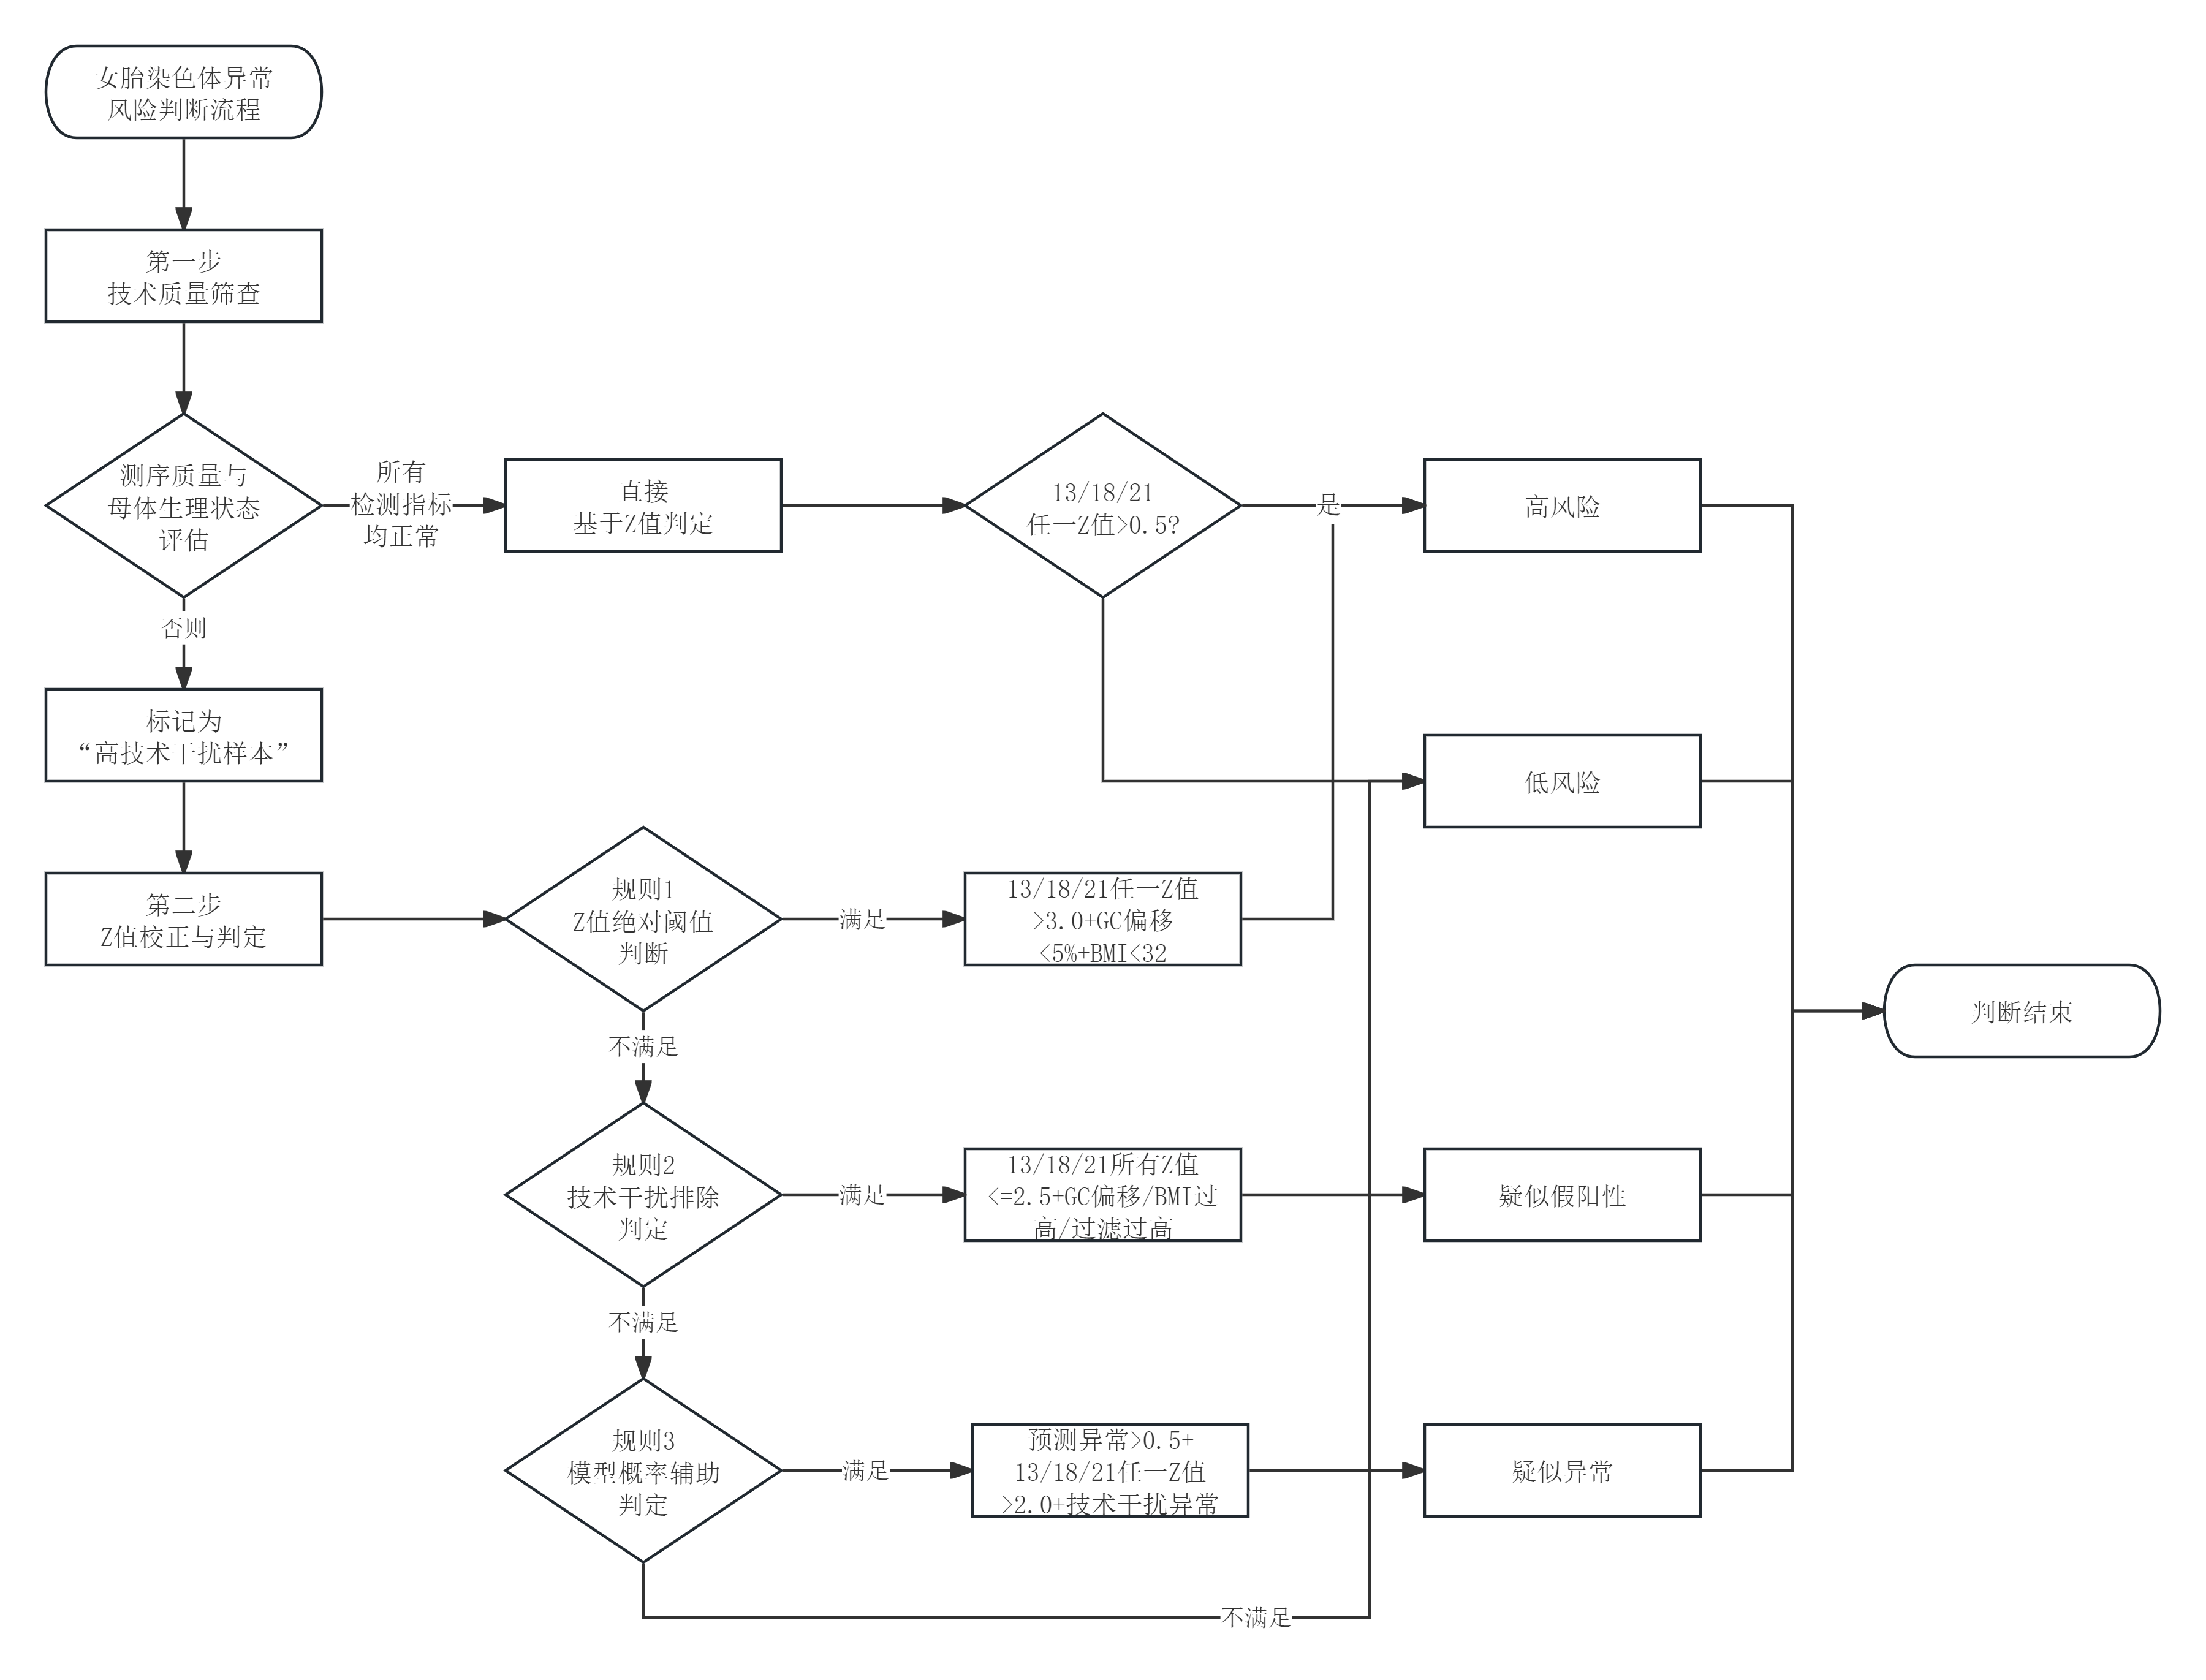
\includegraphics[width=0.8\textwidth]{../figure/q4_flow_chart.png}
    \caption{女胎染色体异常风险判定流程图}
    \label{fig:q4-flow-chart}
\end{figure}

\textbf{第一步:技术质量筛查}
对检测样本进行测序质量与母体生理状态评估:  
若13/18/21号染色体GC含量超出40\%-60\%,或读段过滤率>20\%,或孕妇BMI>30 kg/m² -> 标记为“高技术干扰样本”,进入第二步校正;  
若上述指标均正常 -> 直接基于Z值判定。

\textbf{第二步:Z值校正与判定}
对“高技术干扰样本”,采用以下规则校正并判定:
\begin{enumerate}
    \item Z值绝对值阈值判定:若13/18/21号染色体任一 |Z| > 3.0(严格于常规阈值2.5),且排除GC含量与BMI干扰(如GC含量偏移<5\%,BMI<32) -> 判定为“高风险”,建议进一步行羊水穿刺确诊;
    \item 技术干扰排除判定:若Z值正常(|Z| ≤ 2.5),但存在GC含量偏移、BMI过高或过滤率高 -> 判定为“疑似技术假阳性”,建议1-2周后复测(避开母体生理状态波动期,如控制体重后);
    \item 模型概率辅助判定:输入样本特征至逻辑回归模型,若预测异常概率>0.5,且同时满足“|Z| > 2.0 + 技术干扰指标异常” -> 标记为“疑似异常”,需结合临床超声检查综合确认。
\end{enumerate}

(注:流程以“减少假阳性、避免漏诊”为核心目标,优先通过技术指标筛查降低干扰,再结合Z值与模型概率综合判定)


% 模型评价
\section{模型评价}
\subsection{模型优点}

\begin{enumerate}
    \item 多层次建模,贴合数据特性与研究目标。
    \item 数据预处理严谨,保障模型可靠性。
    \item 全流程采用严格的数据清洗与验证策略,为建模提供高质量输入。
    \item 全面的模型验证与稳健性分析,通过多维度验证确保模型结论可信,避免过拟合与偶然性。
\end{enumerate}

\subsection{模型缺点}
\begin{enumerate}
    \item 部分模型拟合优度与预测能力有限,受数据特性与变量选择限制,部分模型对数据变异的解释力和预测精度有待提升。
    \item 分组与变量选择存在局限性,模型的分组策略与特征体系仍依赖经验,未能完全实现数据驱动的最优解。
    \item 未充分考虑动态变化与个体异质性,模型多基于“单次检测数据”静态建模,忽略了孕期内变量的动态演化与个体特异性。
    \item 样本分布不均衡影响模型泛化能力,数据集中高BMI样本占比过高,低BMI、异常样本不足,导致模型对小众群体的适用性受限。
\end{enumerate}


% 摘要
\bibliography{ref}

% 附录

\begin{appendices}
    \section{中间结果图表}
        \begin{figure}[H]
        \centering
        \begin{minipage}{0.49\textwidth}
            \centering
            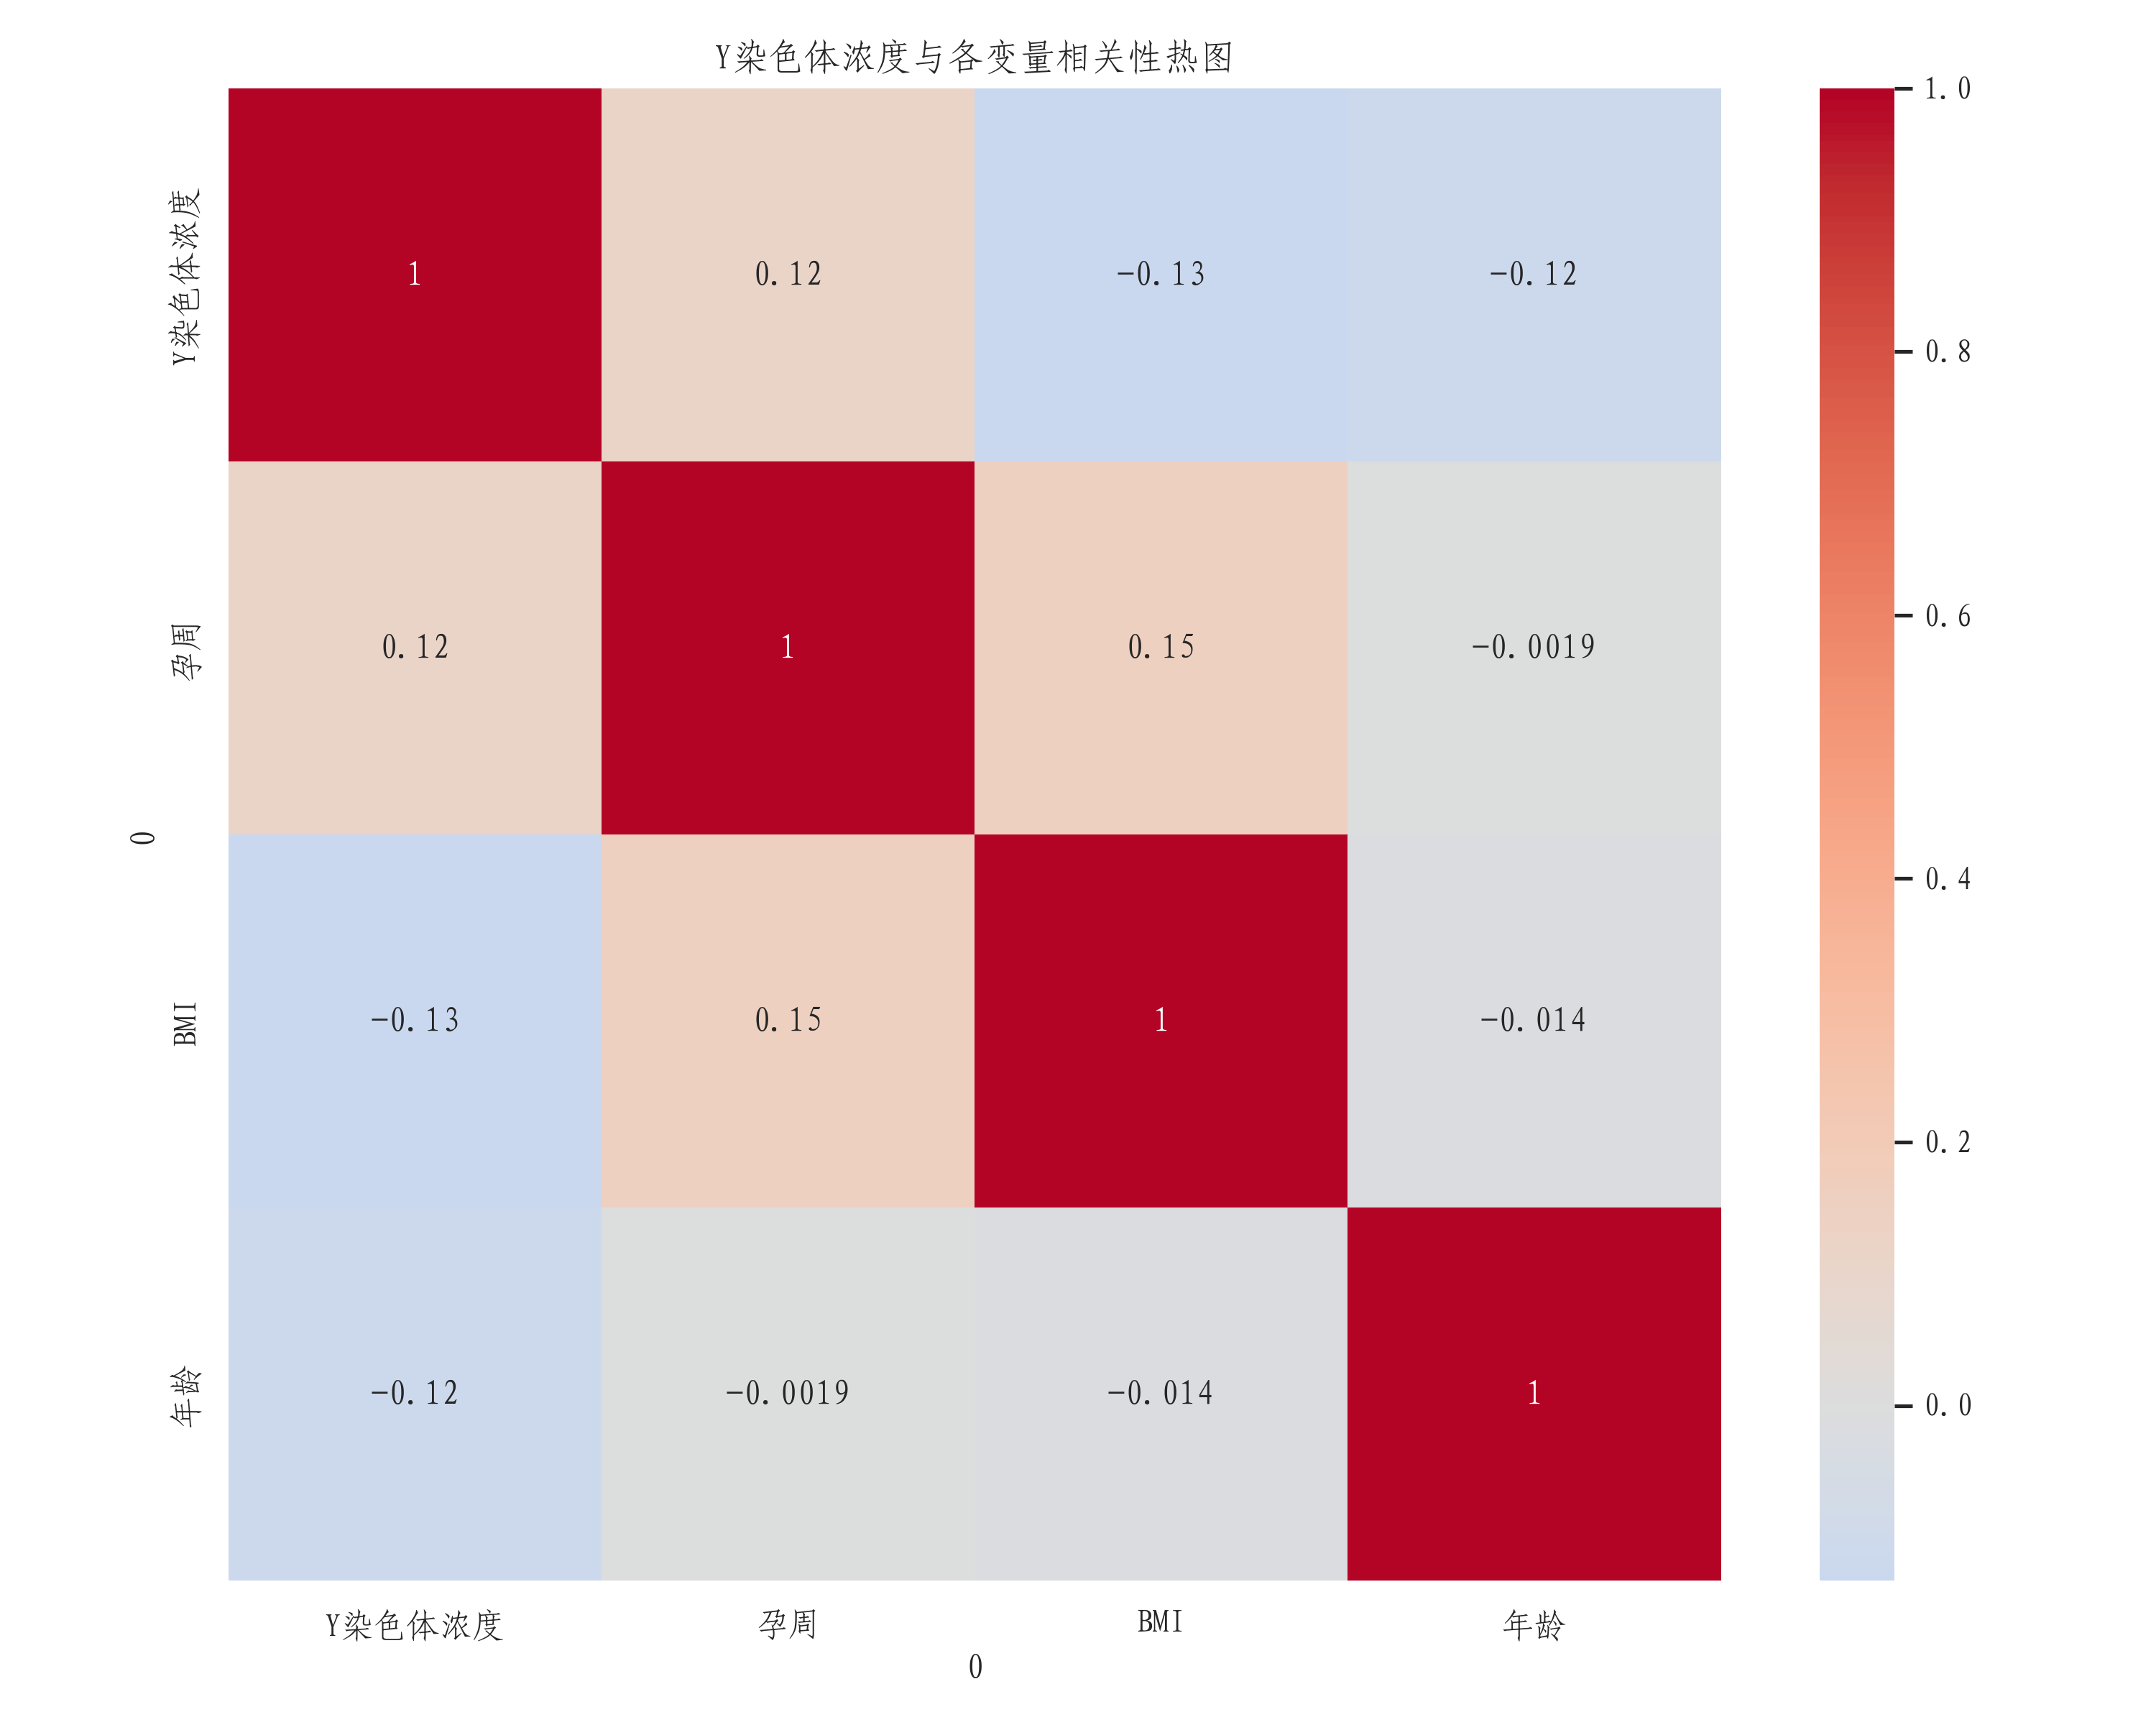
\includegraphics[width=\textwidth]{../figure/C1_Output/correlation_heatmap.png}
        \end{minipage}
        \begin{minipage}{0.49\textwidth}
            \centering
            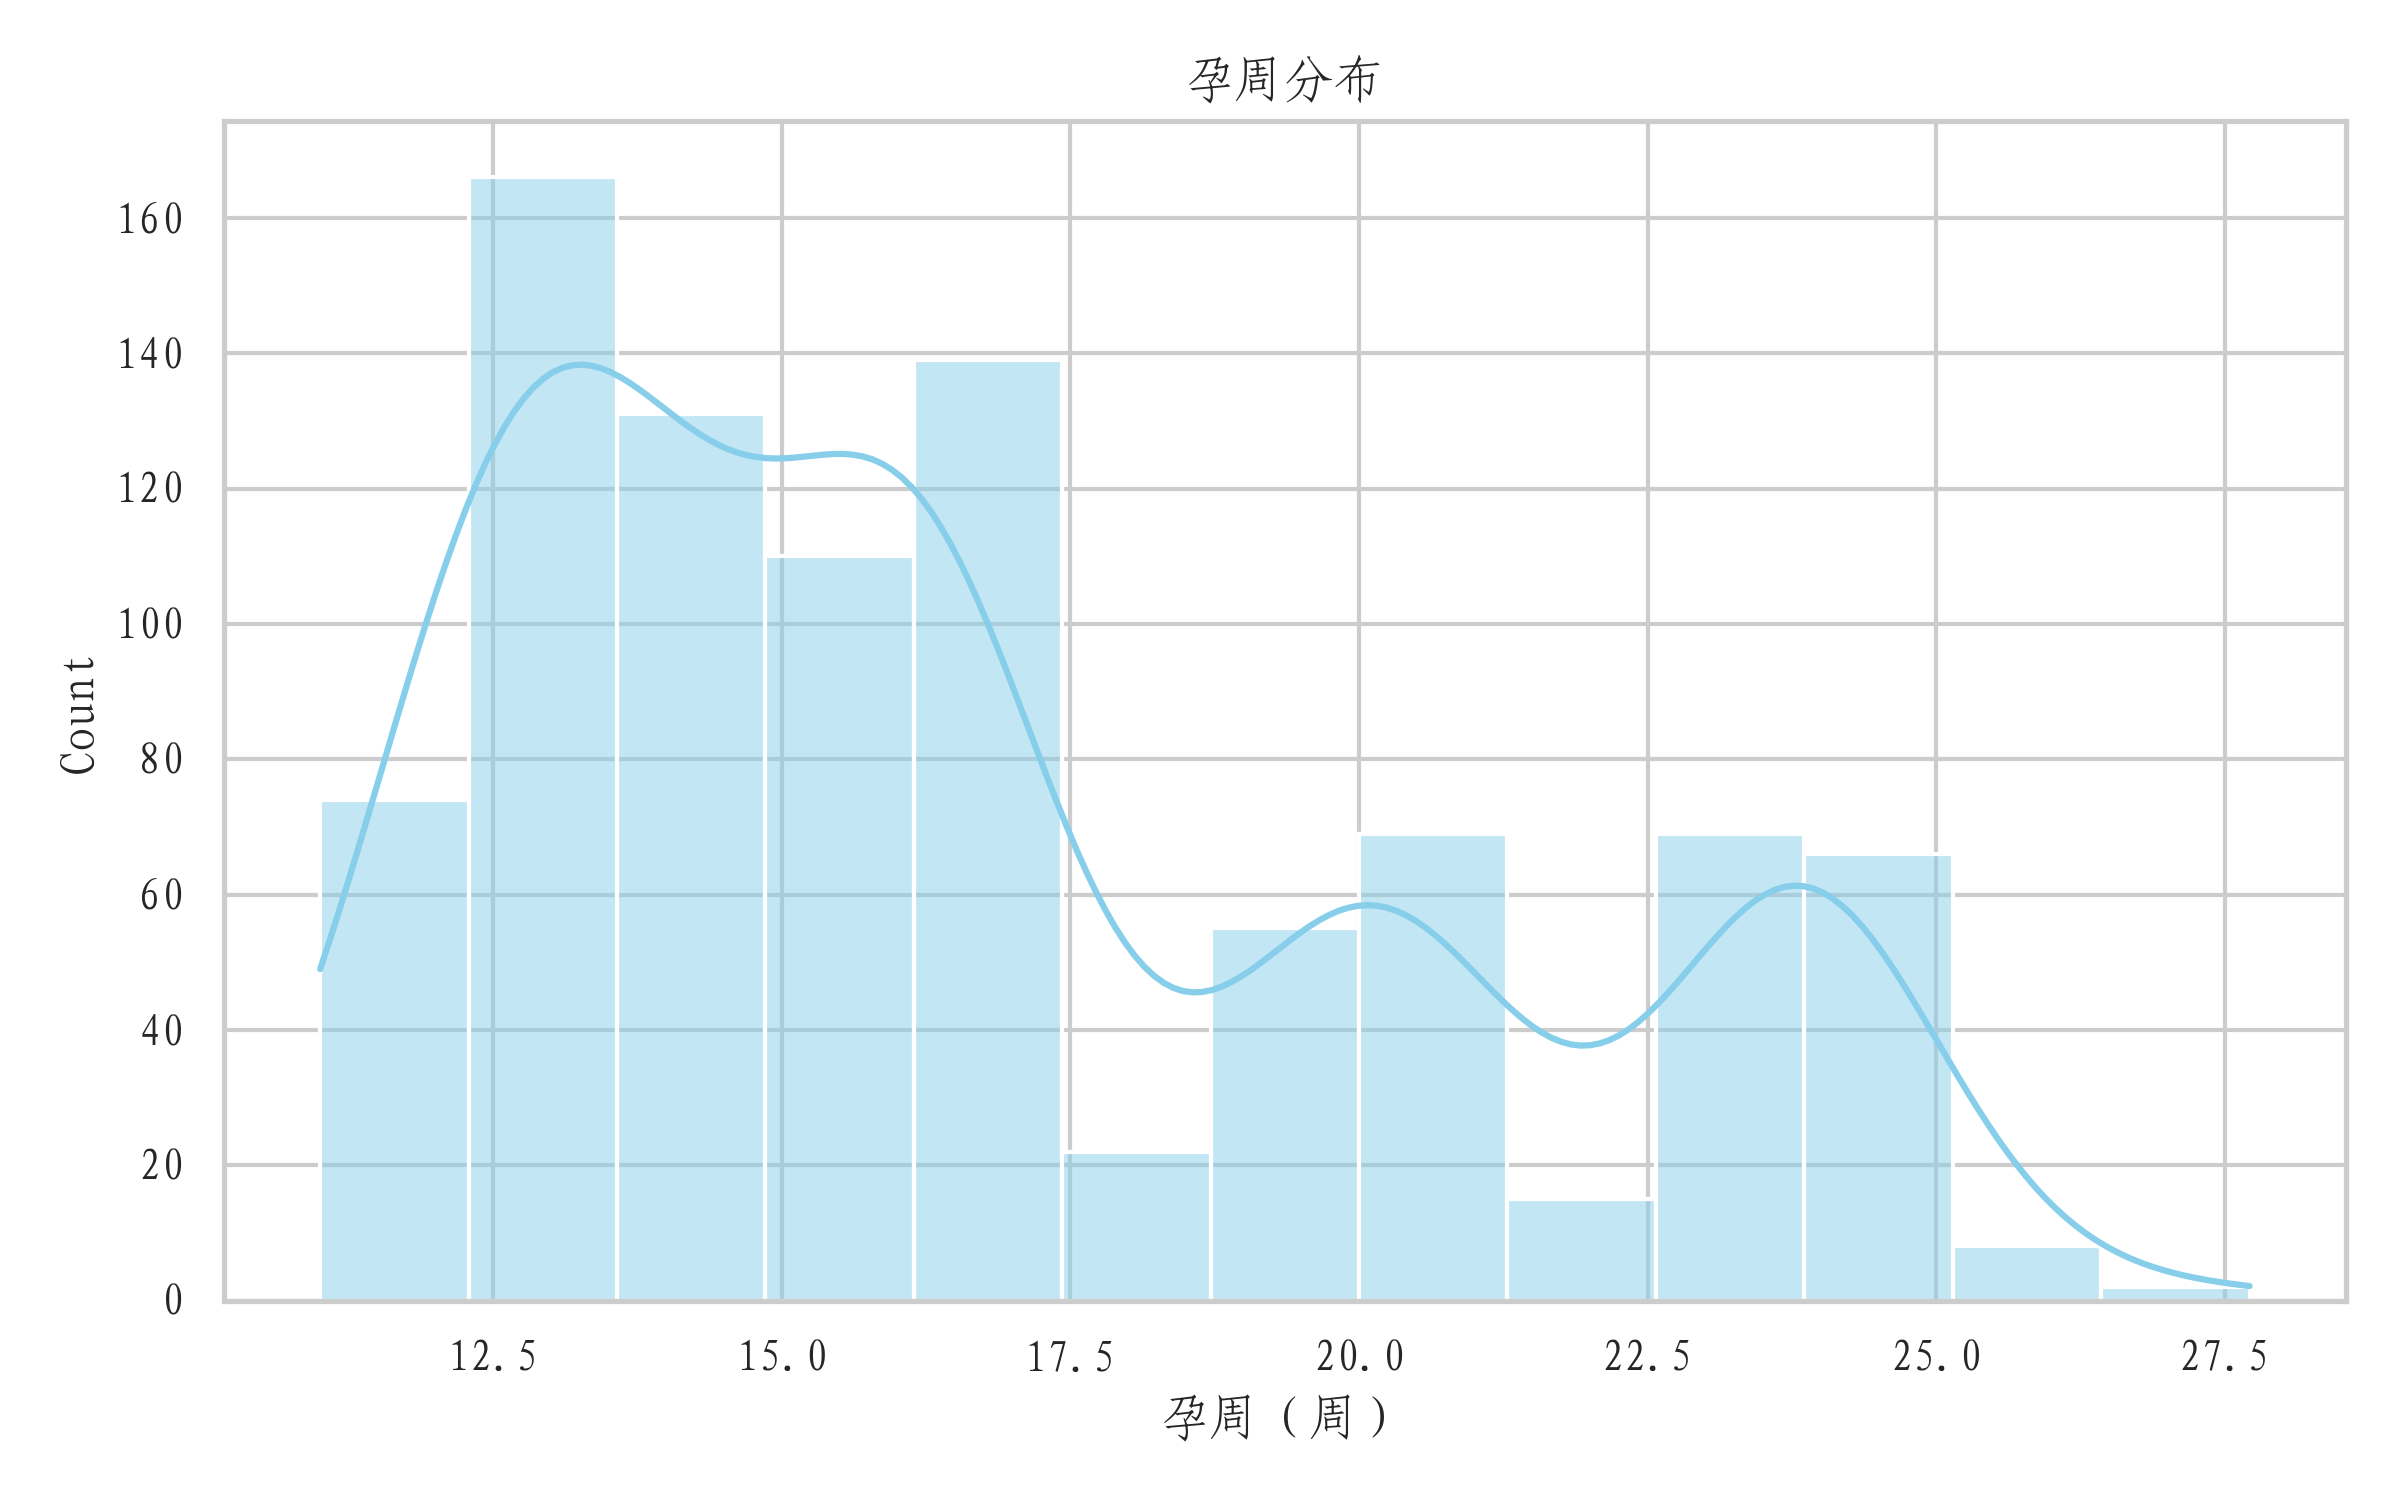
\includegraphics[width=\textwidth]{../figure/C1_Output/hist_gestational_week.png}
        \end{minipage}
        \begin{minipage}{0.49\textwidth}
            \centering
            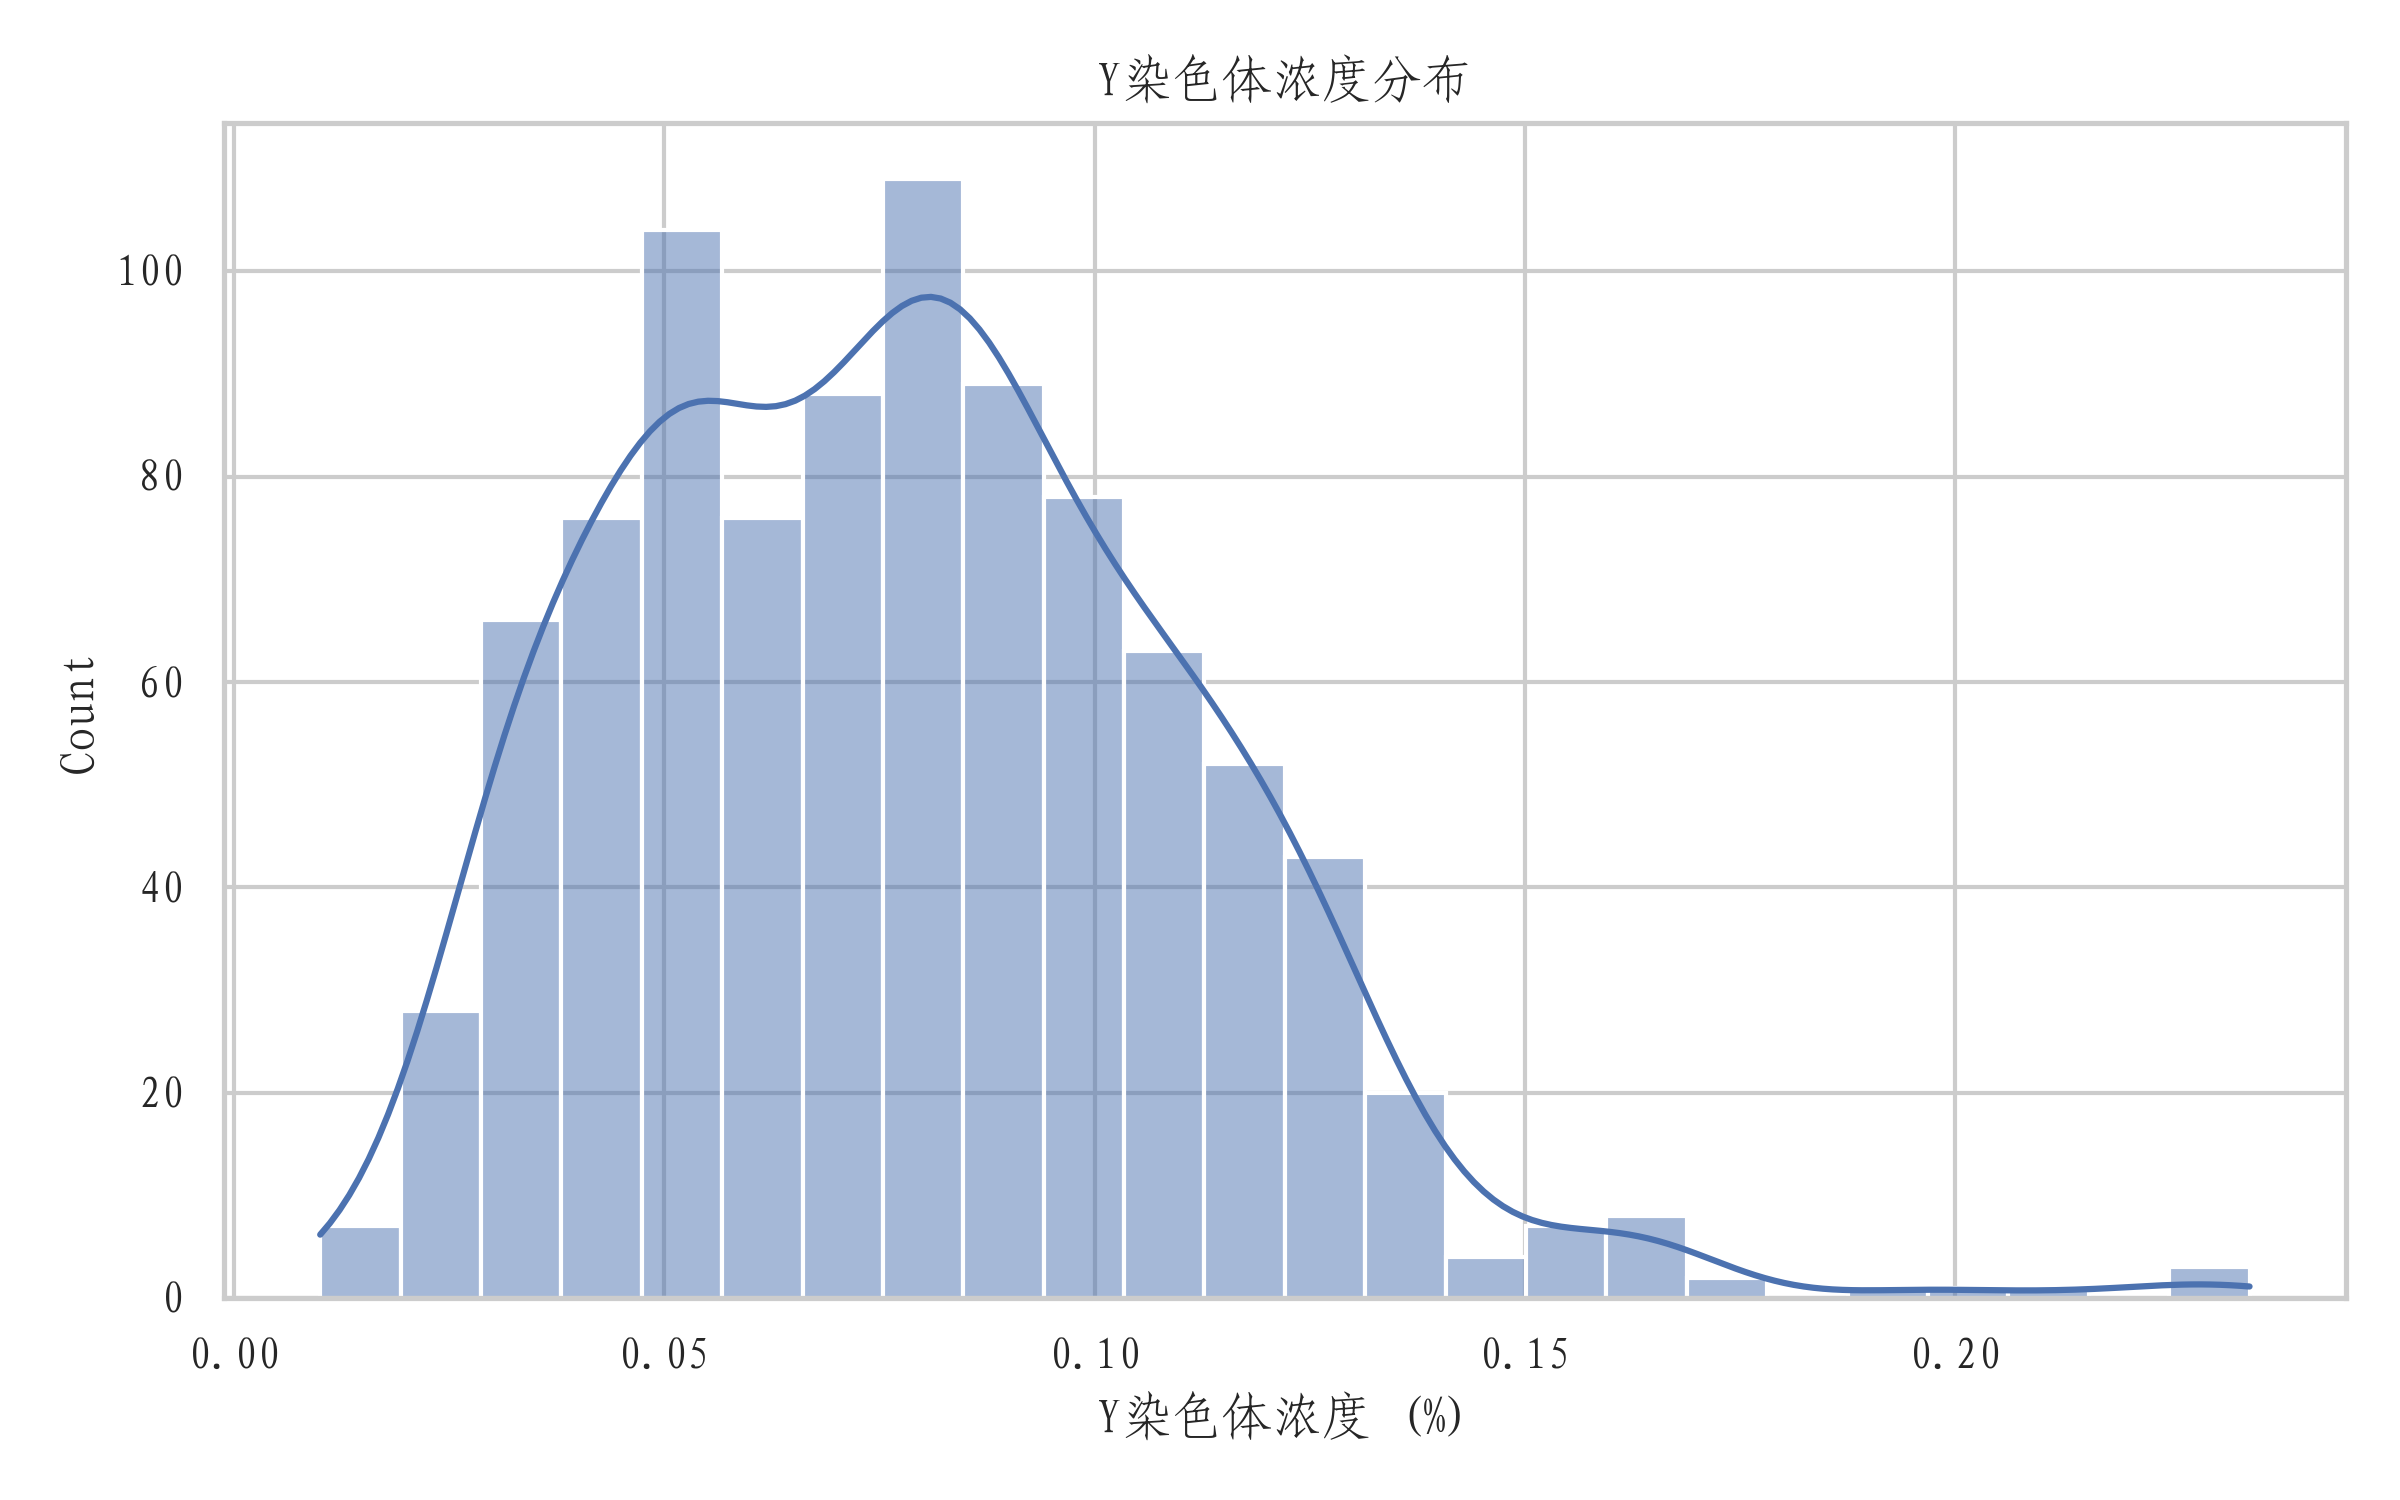
\includegraphics[width=\textwidth]{../figure/C1_Output/hist_y_concentration.png}
        \end{minipage}
        \caption{问题一相关图表-1}
        \label{fig:q1-1}
    \end{figure}

    \begin{figure}[H]
        \centering
        \begin{minipage}{0.49\textwidth}
            \centering
            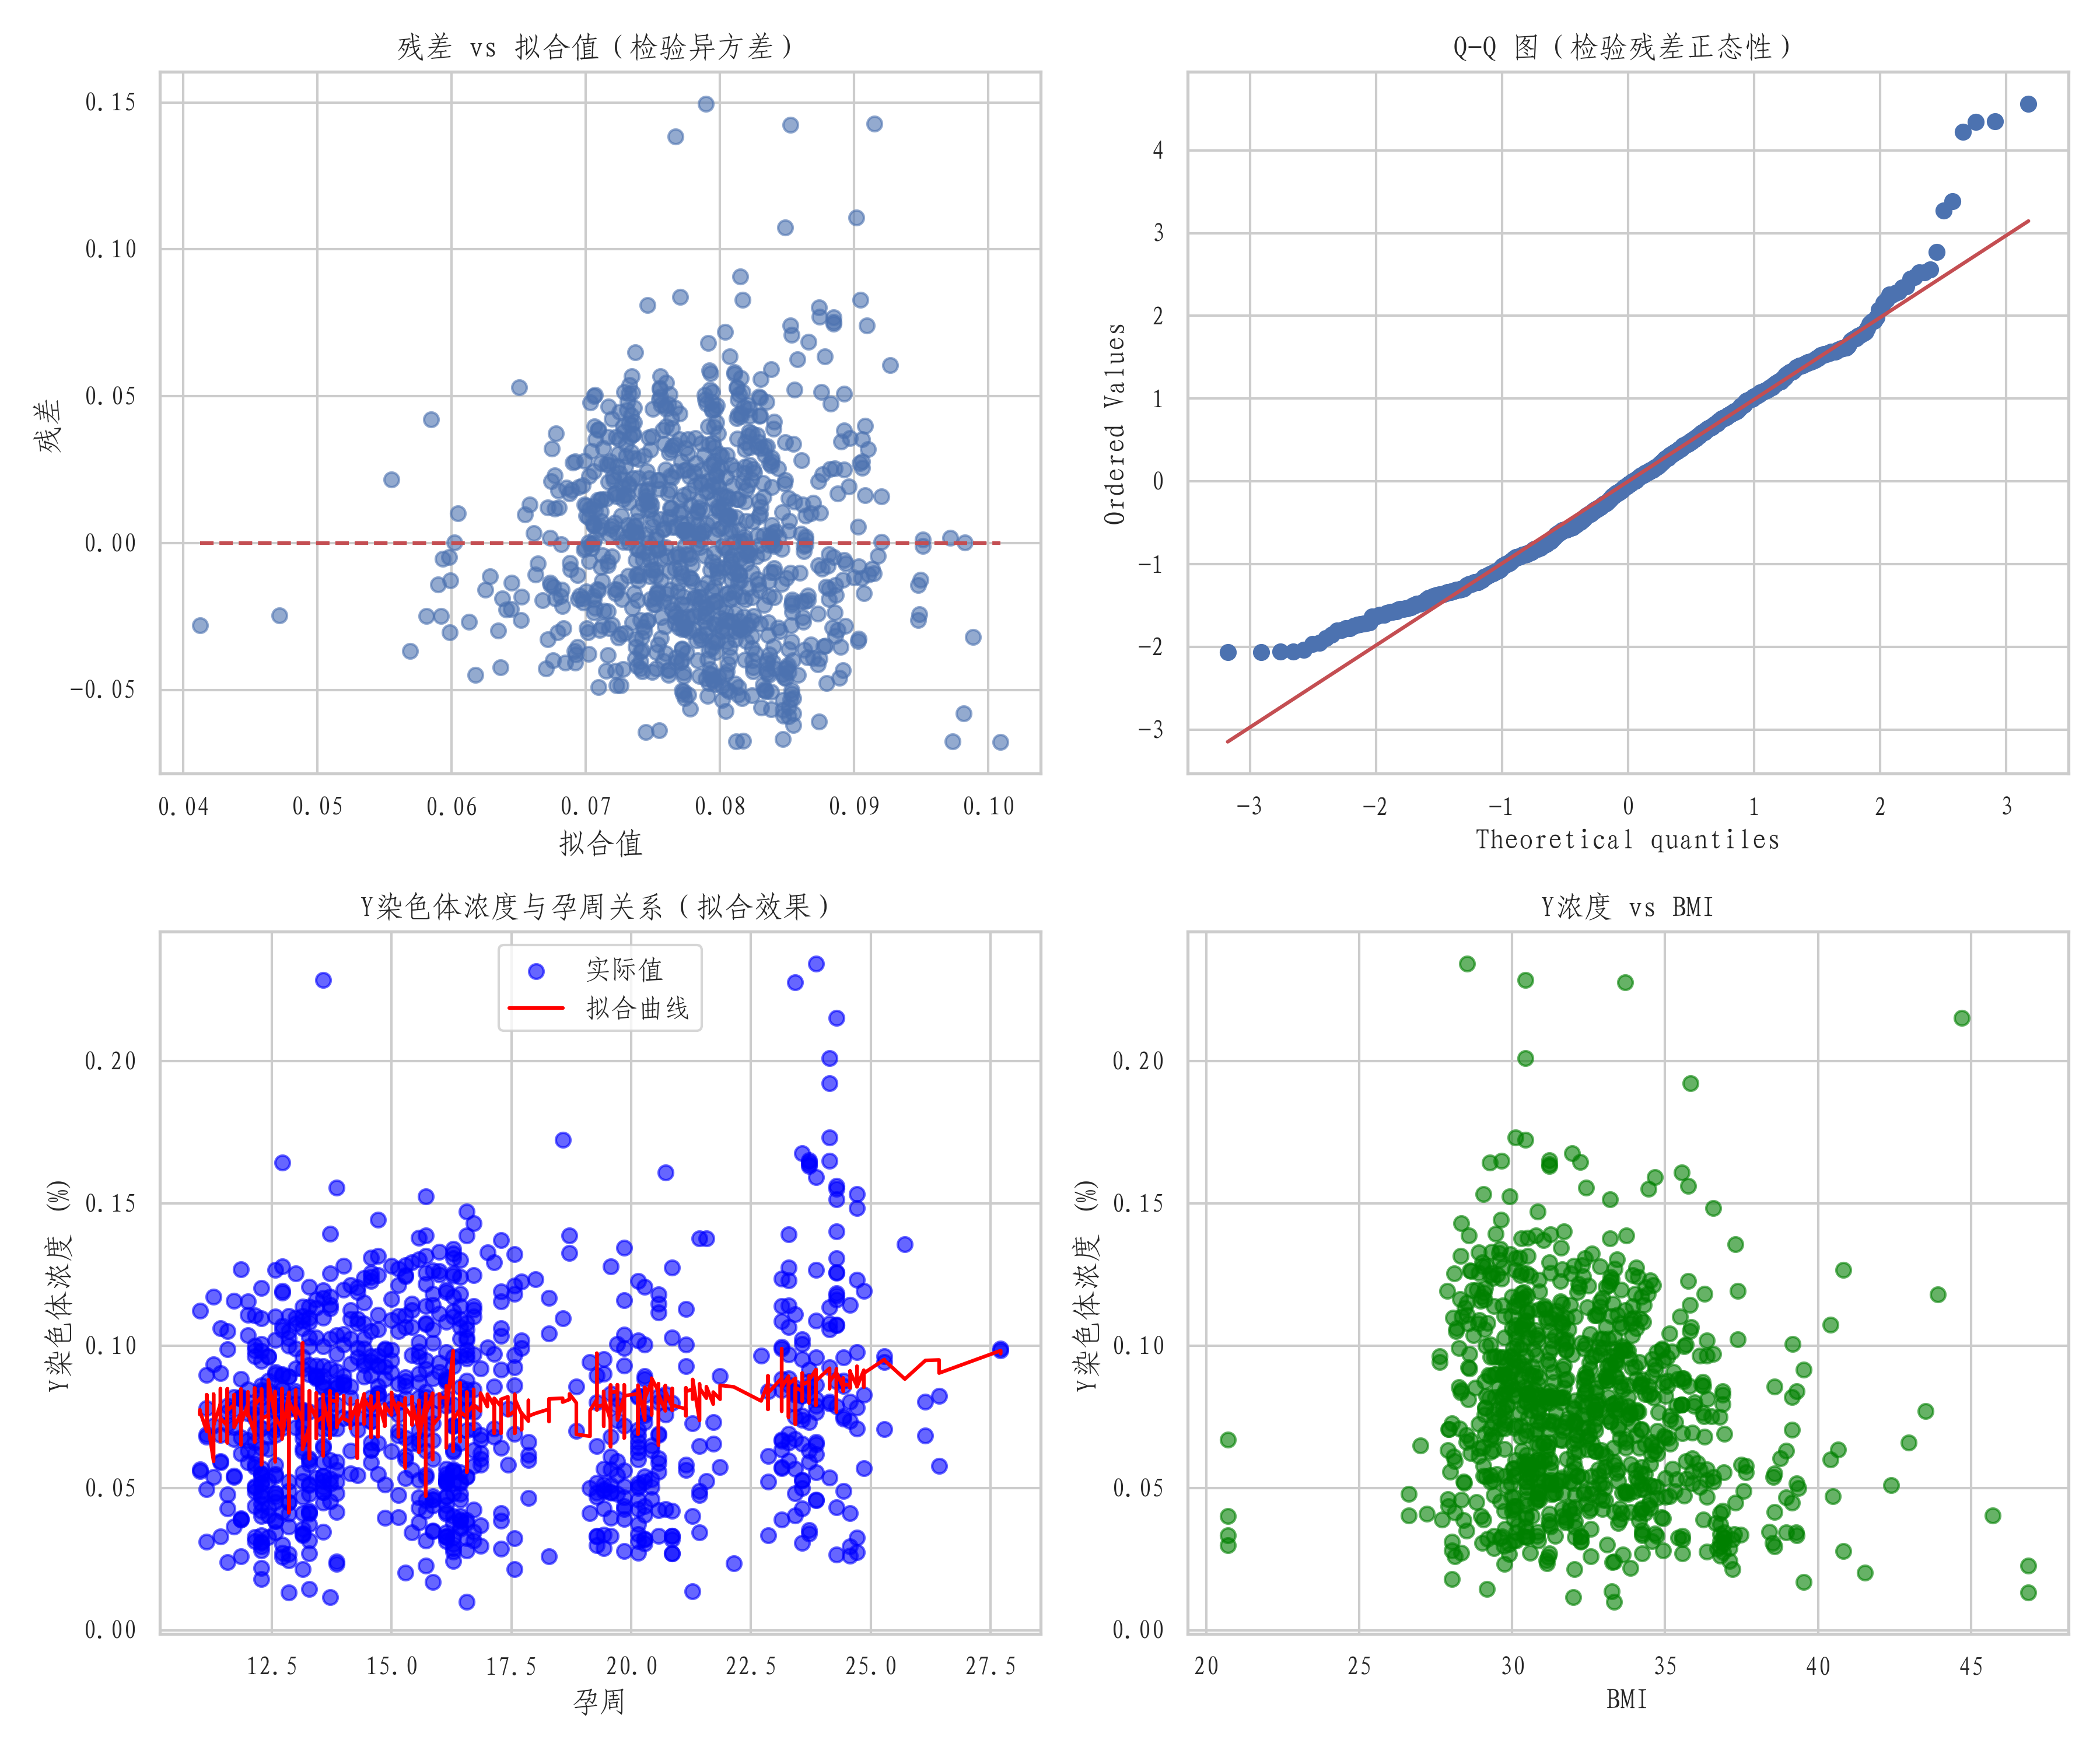
\includegraphics[width=\textwidth]{../figure/C1_Output/residual_diagnostics.png}
        \end{minipage}
        \begin{minipage}{0.49\textwidth}
            \centering
            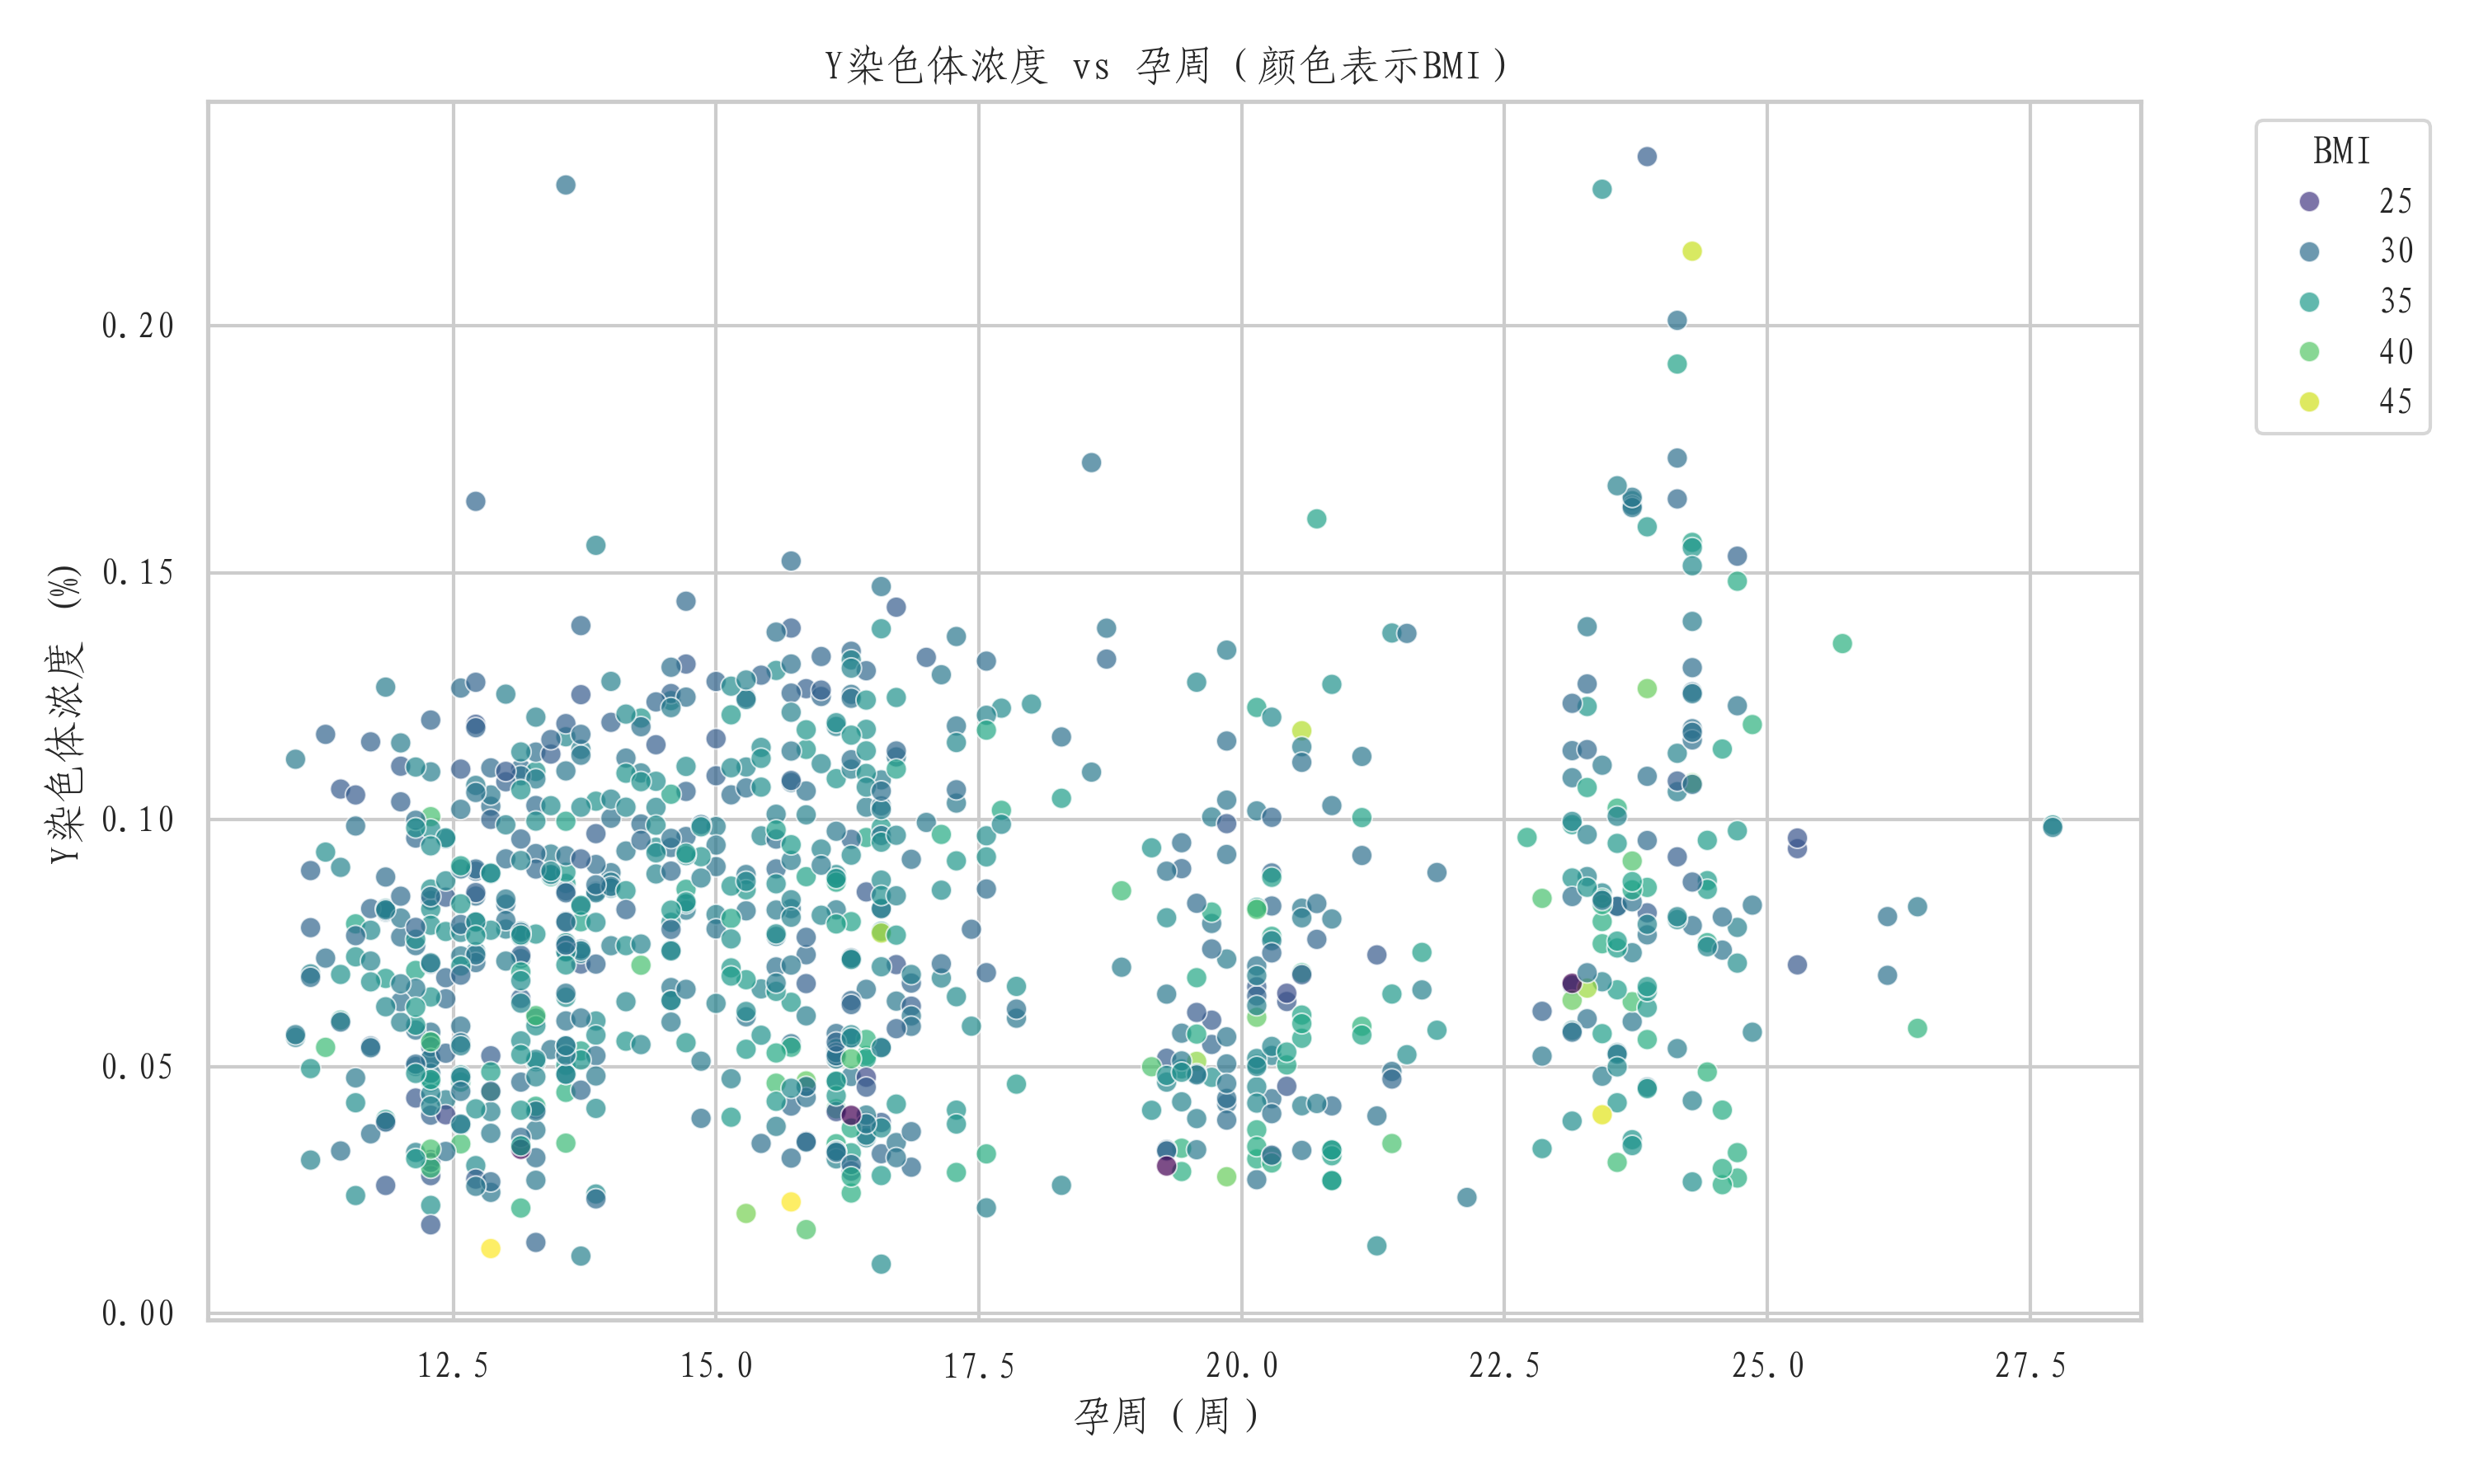
\includegraphics[width=\textwidth]{../figure/C1_Output/scatter_y_vs_gw_by_bmi.png}
        \end{minipage}
        \caption{问题一相关图表-2}
        \label{fig:q1-2}
    \end{figure}

     \begin{figure}[H]
        \centering
        \begin{minipage}{0.49\textwidth}
            \centering
            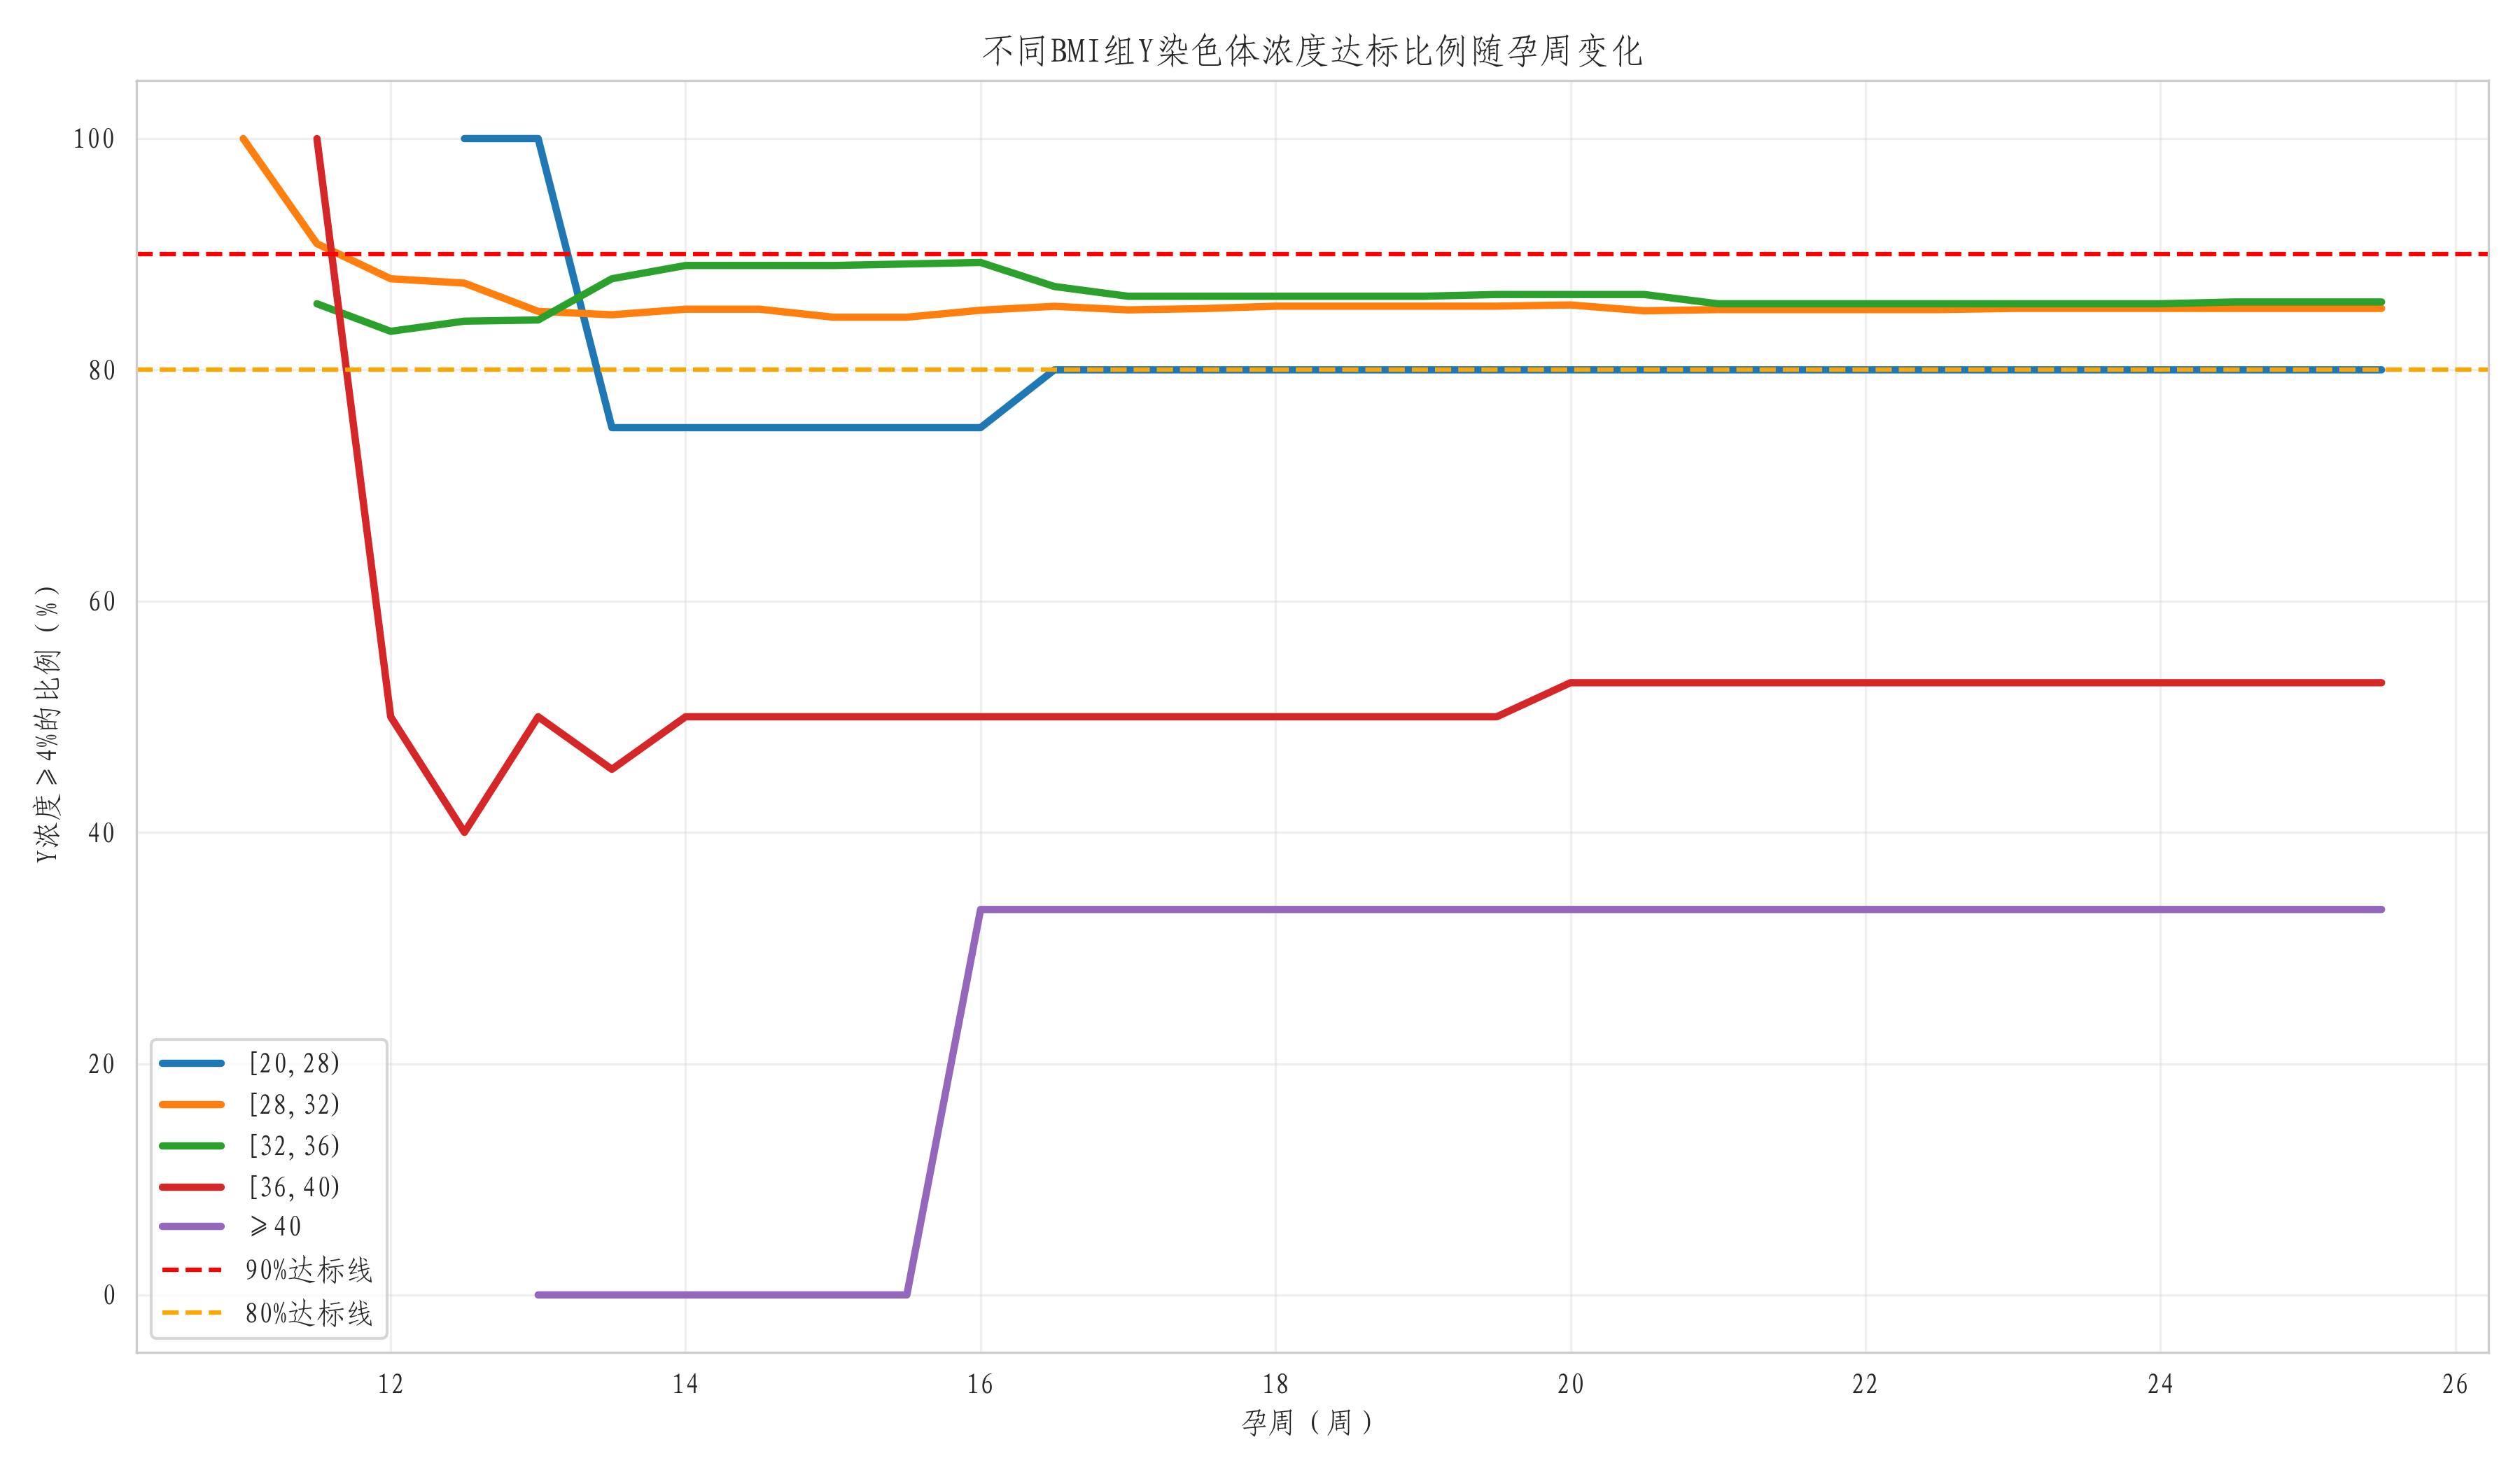
\includegraphics[width=\textwidth]{../figure/C2_Output/attainment_ratio_by_bmi.png}
        \end{minipage}
        \begin{minipage}{0.49\textwidth}
            \centering
            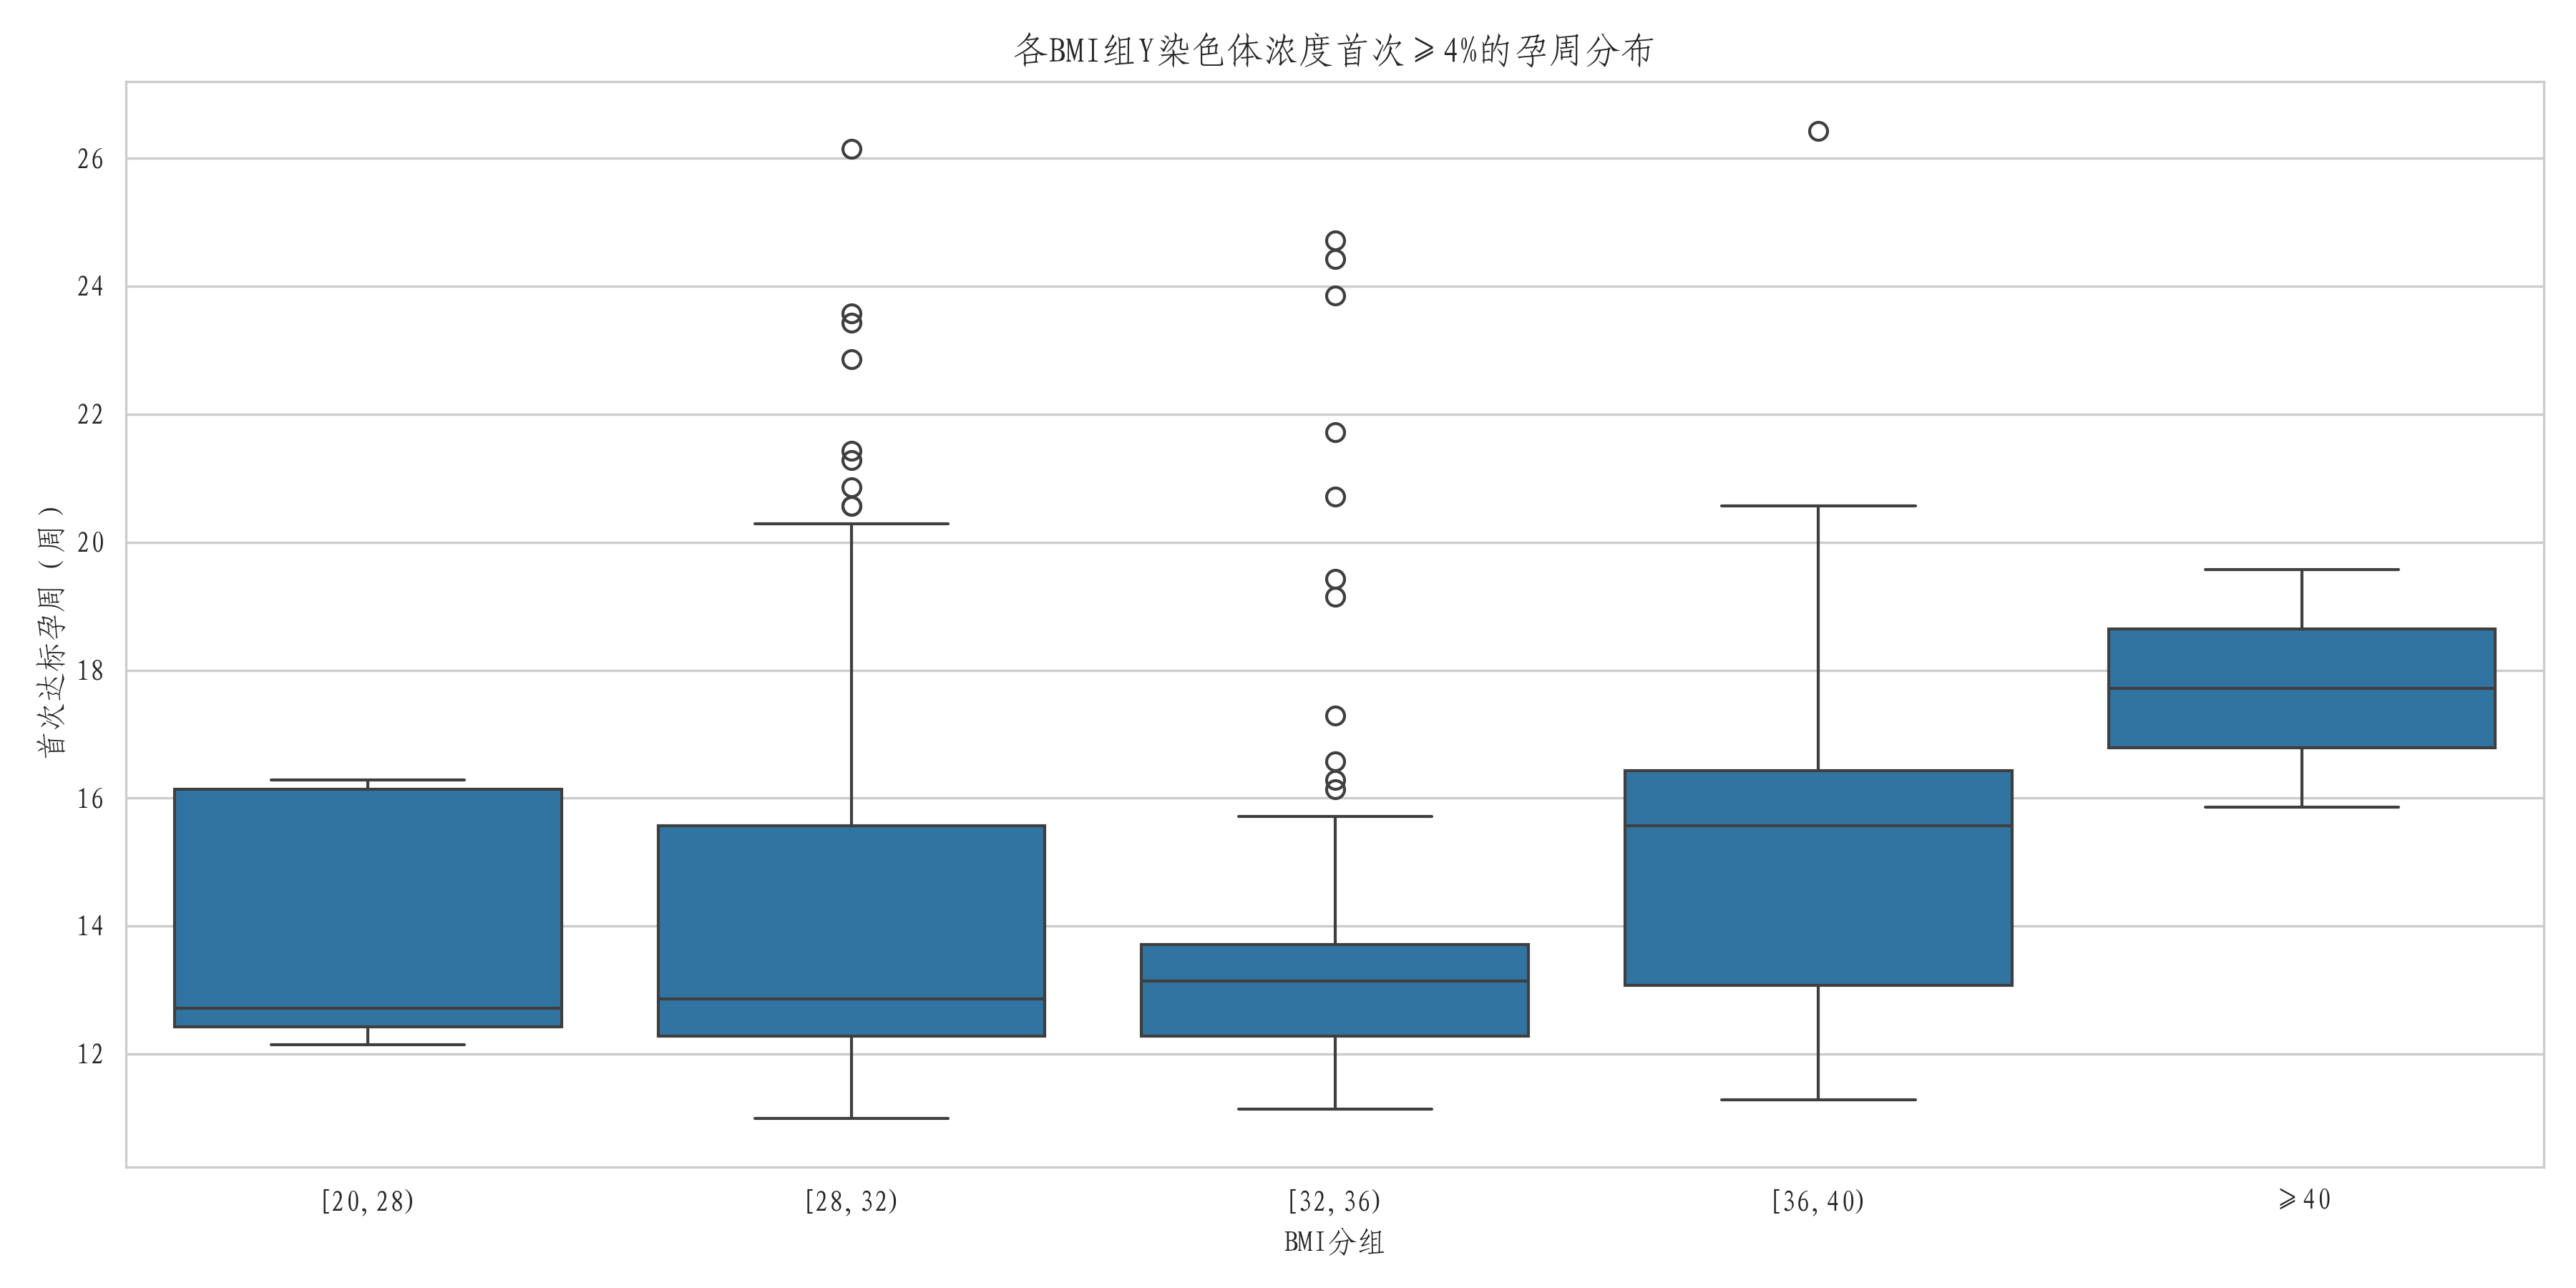
\includegraphics[width=\textwidth]{../figure/C2_Output/first_attainment_by_bmi.png}
        \end{minipage}
        \caption{问题二相关图表}
        \label{fig:q2}
    \end{figure}
    \begin{figure}[H]
        \centering
        \begin{minipage}{0.49\textwidth}
            \centering
            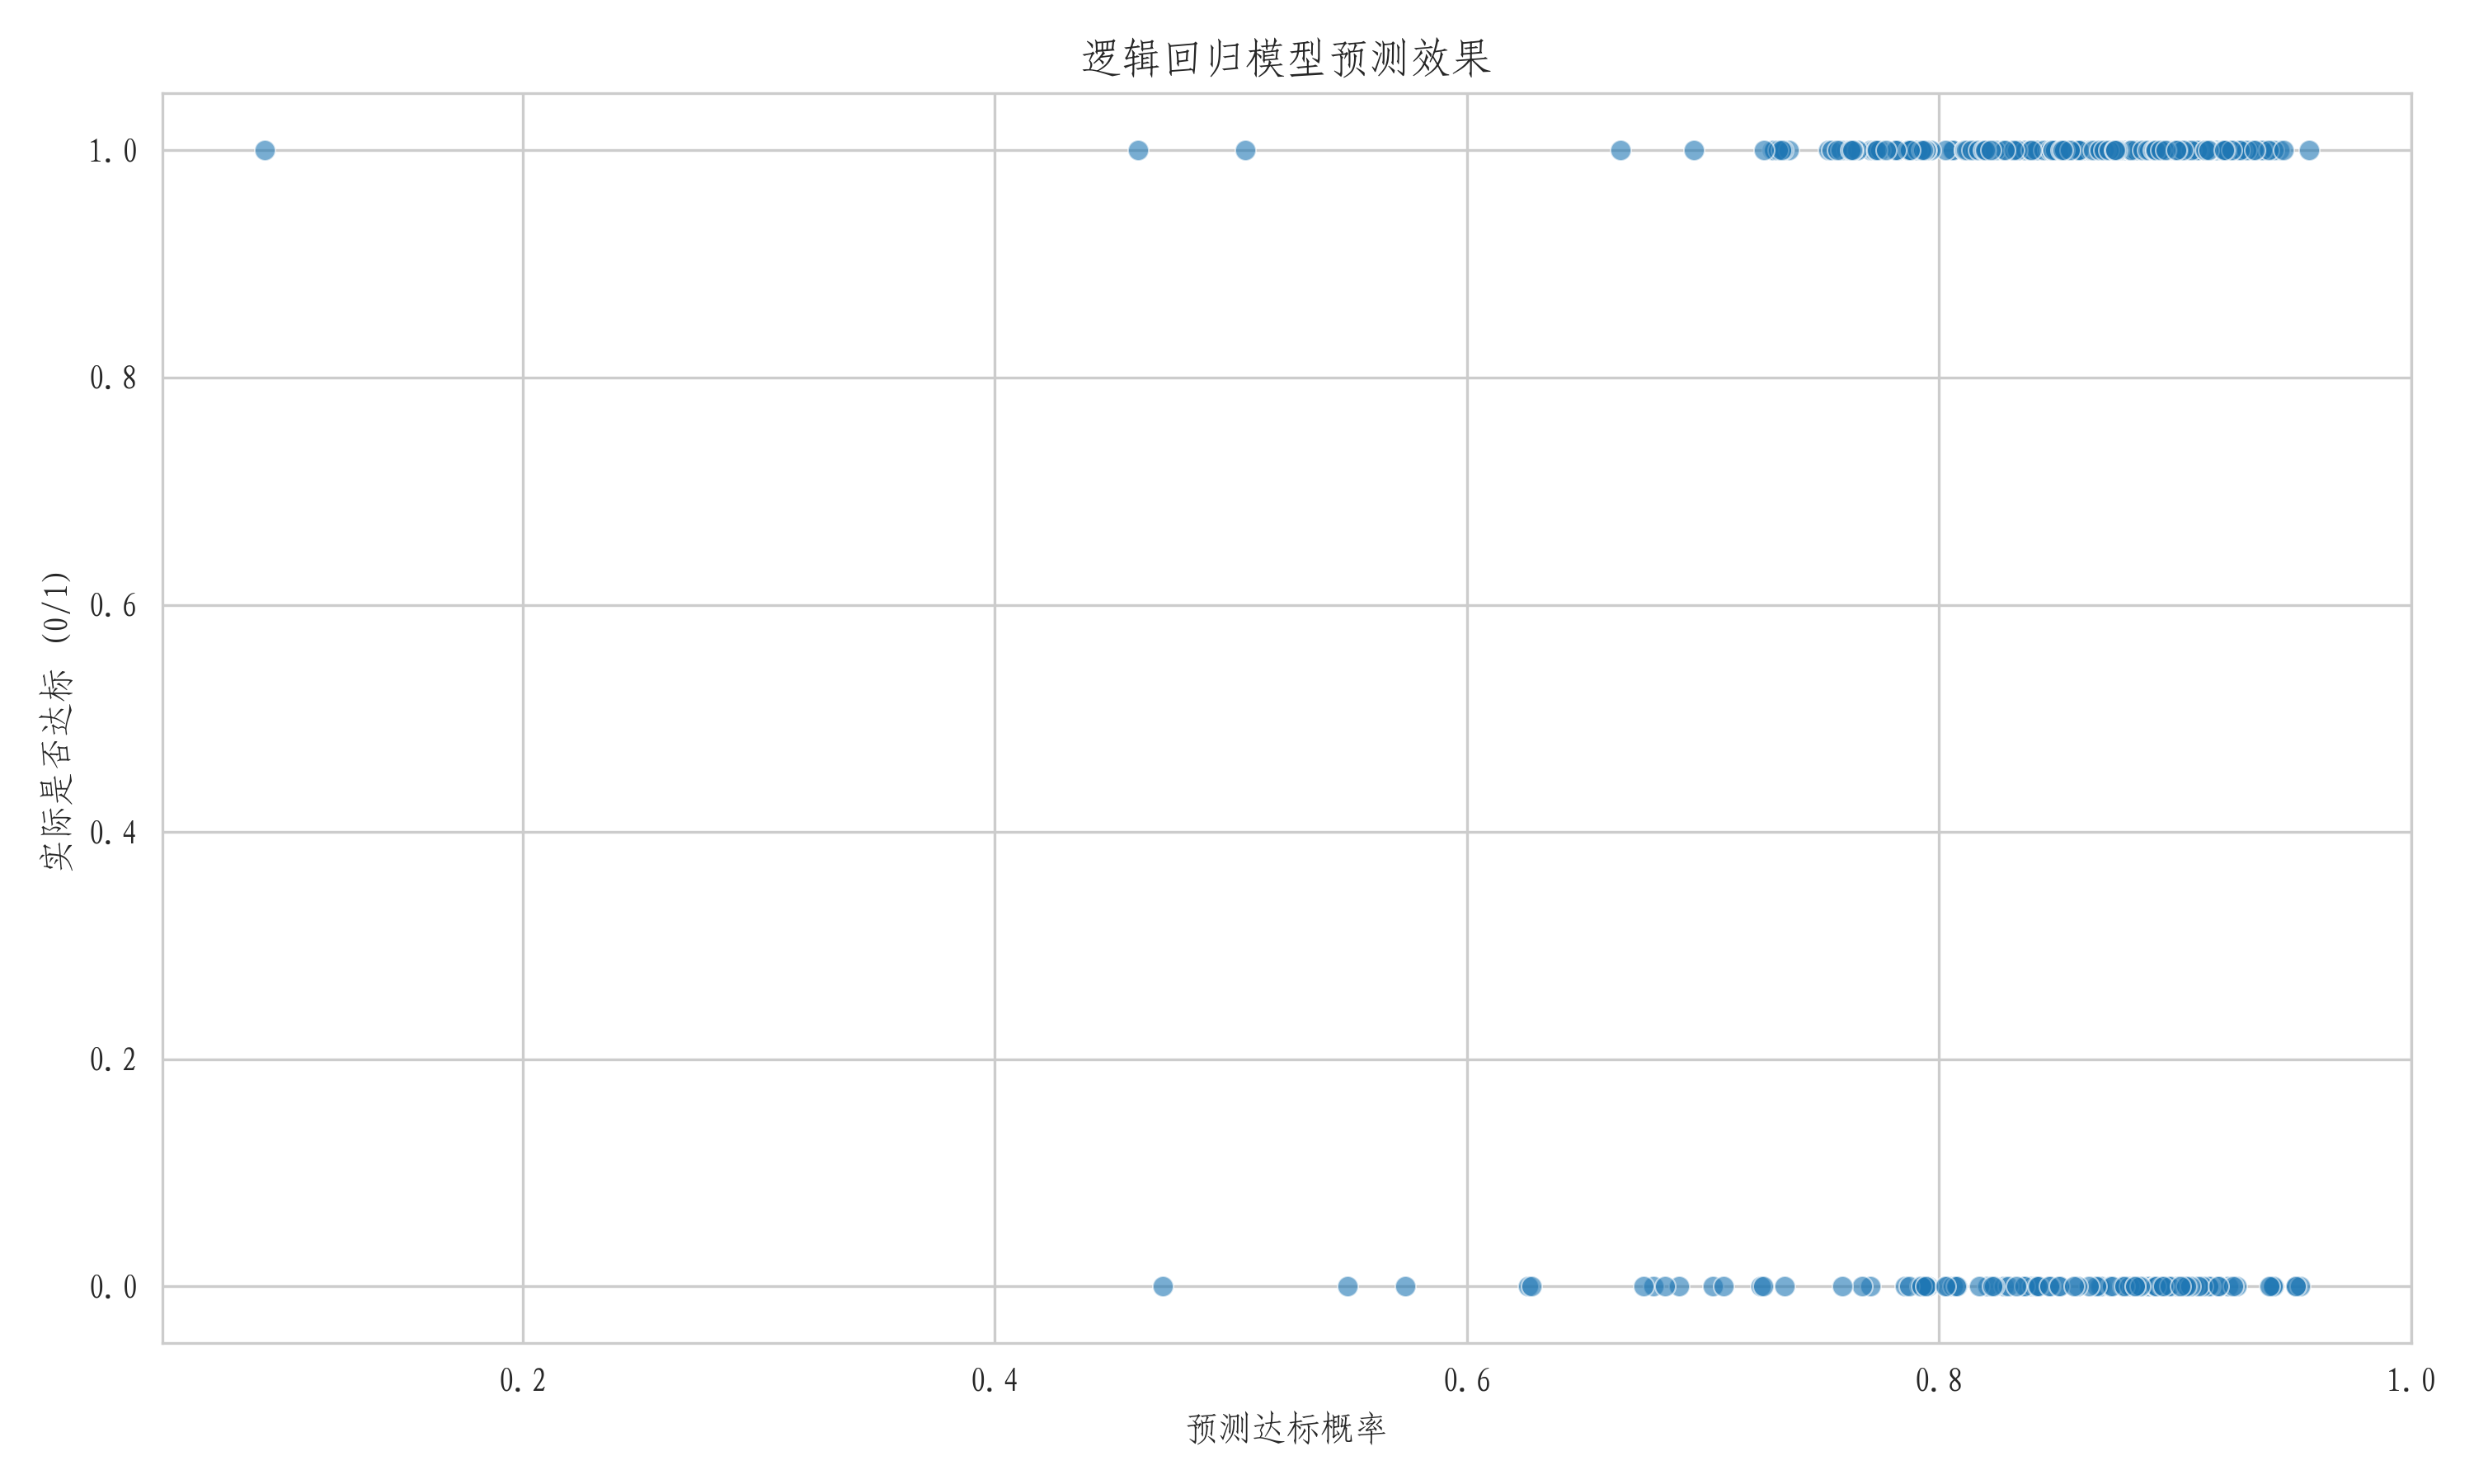
\includegraphics[width=\textwidth]{../figure/C3_Output/logit_prediction_scatter.png}
        \end{minipage}
        \begin{minipage}{0.49\textwidth}
            \centering
            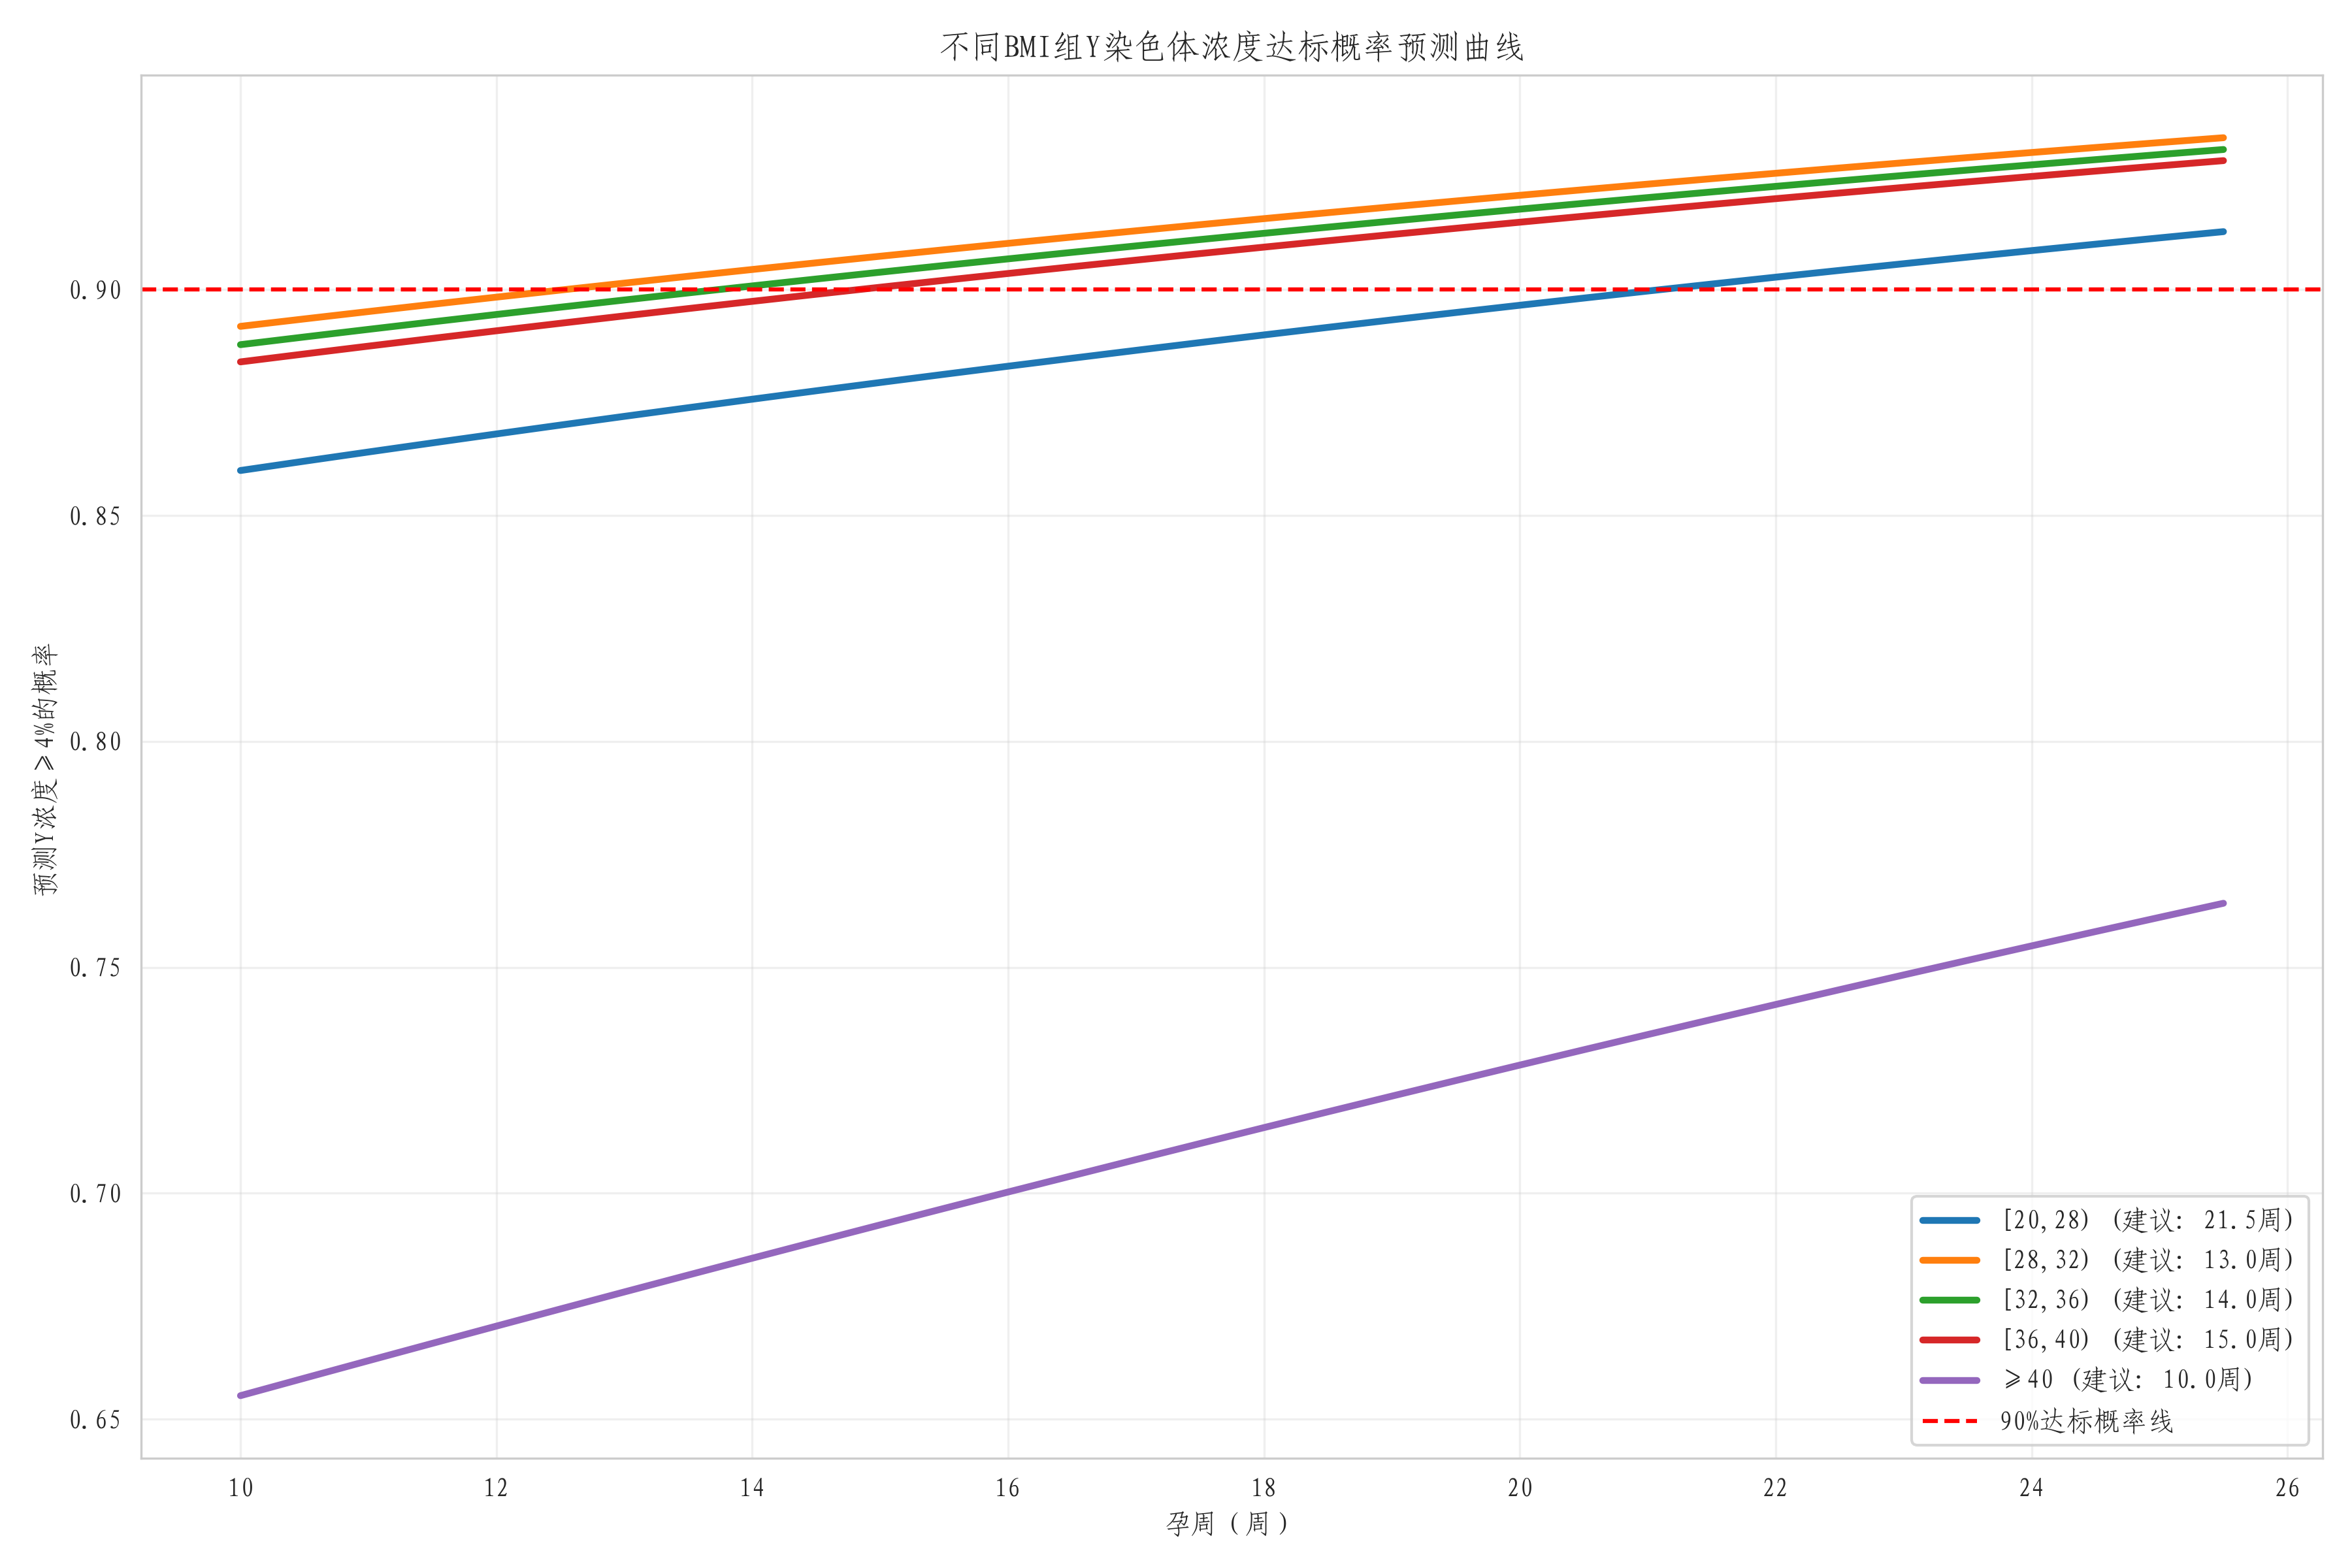
\includegraphics[width=\textwidth]{../figure/C3_Output/predicted_attainment_curve.png}
        \end{minipage}
        \caption{问题三相关图表}
        \label{fig:q3}
    \end{figure}

     \begin{figure}[H]
        \centering
        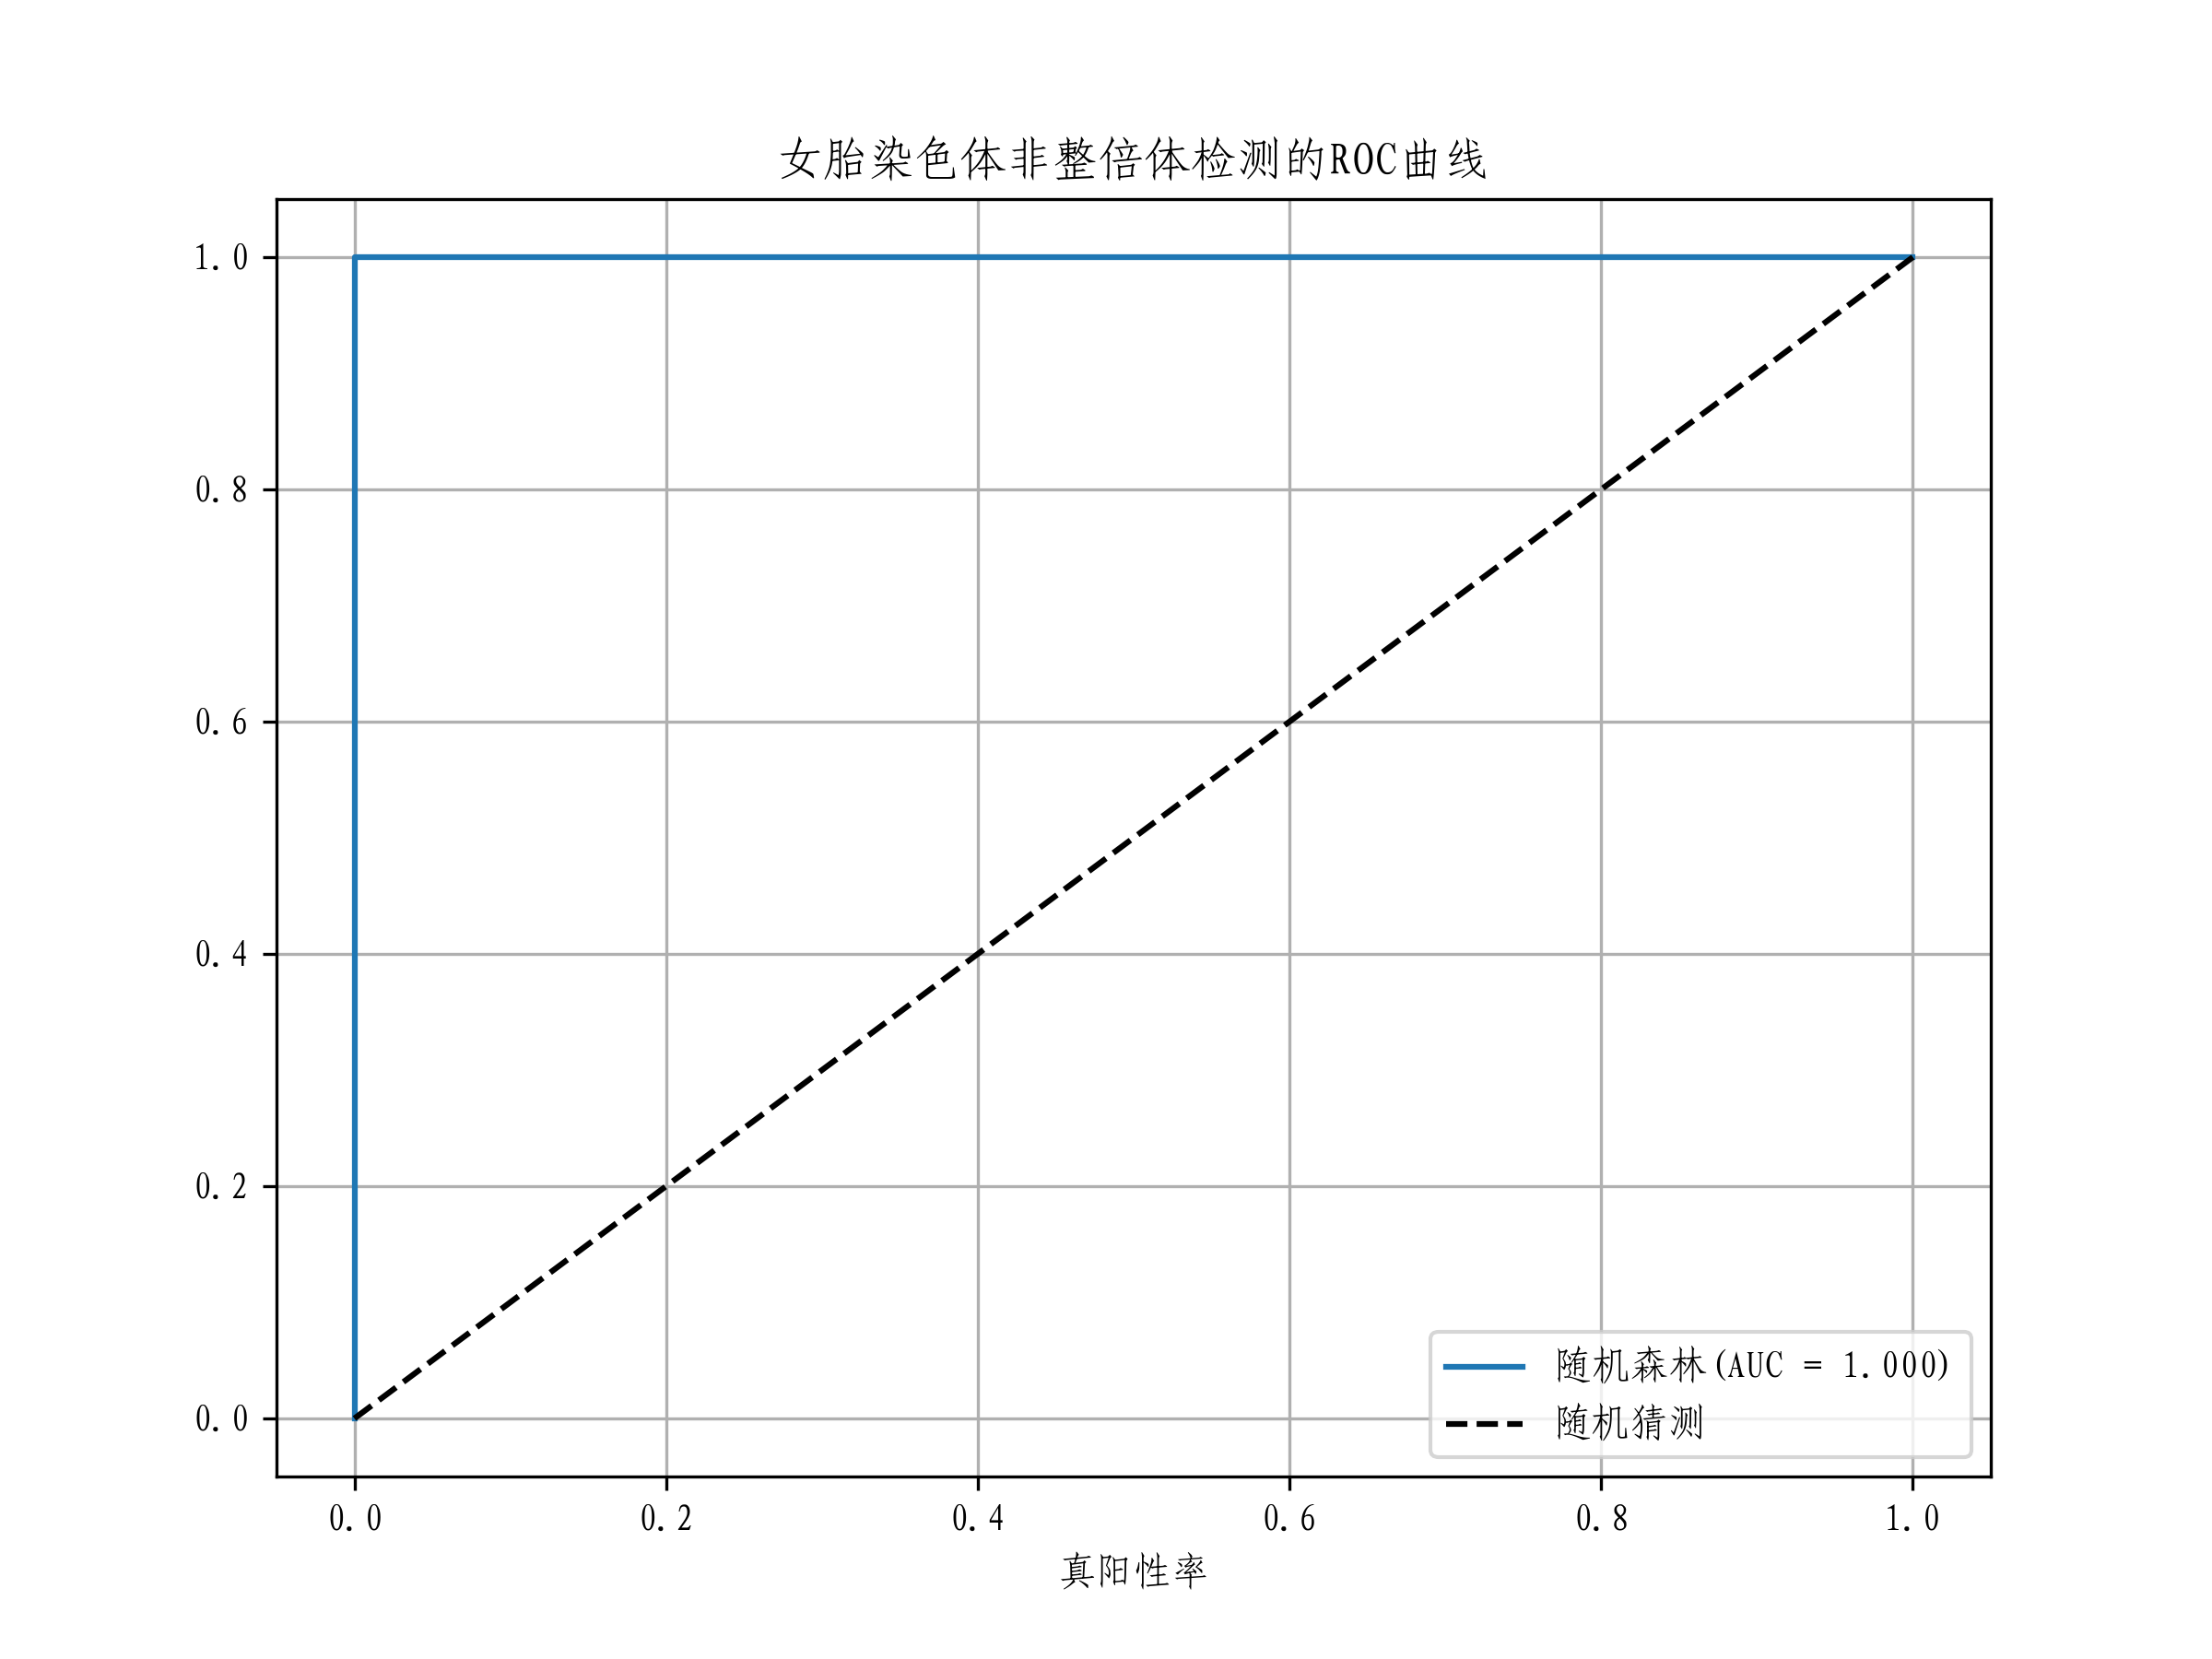
\includegraphics[width=0.8\textwidth]{../figure/C4_Output/roc_curve_for_female_fetal_aneuploidy_detection.png}
        \caption{问题四相关图表}
        \label{fig:q4}
    \end{figure}



    \section{文件列表}
    \begin{table}[H]
        \caption{程序文件列表}
        \centering
        \begin{tabularx}{\textwidth}{l l}
            \bottomrule[1.5pt]
            文件名 & 功能描述 \\
            \midrule[1pt]
            附件.xlsx & 题目给定的原始数据\\
            附件 - 男胎检测数据.xlsx & 原始数据拆解得到的男胎检测数据表 \\
            附件 - 女胎检测数据.xlsx & 原始数据拆解得到的女胎检测数据表 \\
            仿宋\_GB2312.TTF & 使用的中文字体文件 \\
            times.ttf & 使用的英文字体文件 \\
            code1.py & 问题一程序代码 \\
            code2.py & 问题二程序代码 \\
            code3.py & 问题三程序代码 \\
            code4.py & 问题四程序代码 \\
            C1\_Output & 问题一中间结果文件夹 \\
            C2\_Output & 问题二中间结果文件夹 \\
            C3\_Output & 问题三中间结果文件夹 \\
            C4\_Output & 问题四中间结果文件夹 \\
            \bottomrule[1.5pt]
        \end{tabularx}
        \label{tab:文件列表}
    \end{table}



    \section{代码}
    \subsection{问题1代码}
        \lstinputlisting[language=python]{../code/code1.py}    
    \subsection{问题2代码}
        \lstinputlisting[language=python]{../code/code2.py}
    \subsection{问题3代码}
        \lstinputlisting[language=python]{../code/code3.py}
    \subsection{问题4代码}
        \lstinputlisting[language=python]{../code/code4.py}

\end{appendices}

\end{document}